% Options for packages loaded elsewhere
% Options for packages loaded elsewhere
\PassOptionsToPackage{unicode}{hyperref}
\PassOptionsToPackage{hyphens}{url}
%
\documentclass[
  ignorenonframetext,
]{beamer}
\newif\ifbibliography
\usepackage{pgfpages}
\setbeamertemplate{caption}[numbered]
\setbeamertemplate{caption label separator}{: }
\setbeamercolor{caption name}{fg=normal text.fg}
\beamertemplatenavigationsymbolsempty
% remove section numbering
\setbeamertemplate{part page}{
  \centering
  \begin{beamercolorbox}[sep=16pt,center]{part title}
    \usebeamerfont{part title}\insertpart\par
  \end{beamercolorbox}
}
\setbeamertemplate{section page}{
  \centering
  \begin{beamercolorbox}[sep=12pt,center]{section title}
    \usebeamerfont{section title}\insertsection\par
  \end{beamercolorbox}
}
\setbeamertemplate{subsection page}{
  \centering
  \begin{beamercolorbox}[sep=8pt,center]{subsection title}
    \usebeamerfont{subsection title}\insertsubsection\par
  \end{beamercolorbox}
}
% Prevent slide breaks in the middle of a paragraph
\widowpenalties 1 10000
\raggedbottom
\AtBeginPart{
  \frame{\partpage}
}
\AtBeginSection{
  \ifbibliography
  \else
    \frame{\sectionpage}
  \fi
}
\AtBeginSubsection{
  \frame{\subsectionpage}
}
\usepackage{iftex}
\ifPDFTeX
  \usepackage[T1]{fontenc}
  \usepackage[utf8]{inputenc}
  \usepackage{textcomp} % provide euro and other symbols
\else % if luatex or xetex
  \usepackage{unicode-math} % this also loads fontspec
  \defaultfontfeatures{Scale=MatchLowercase}
  \defaultfontfeatures[\rmfamily]{Ligatures=TeX,Scale=1}
\fi
\usepackage{lmodern}

\ifPDFTeX\else
  % xetex/luatex font selection
\fi
% Use upquote if available, for straight quotes in verbatim environments
\IfFileExists{upquote.sty}{\usepackage{upquote}}{}
\IfFileExists{microtype.sty}{% use microtype if available
  \usepackage[]{microtype}
  \UseMicrotypeSet[protrusion]{basicmath} % disable protrusion for tt fonts
}{}
\makeatletter
\@ifundefined{KOMAClassName}{% if non-KOMA class
  \IfFileExists{parskip.sty}{%
    \usepackage{parskip}
  }{% else
    \setlength{\parindent}{0pt}
    \setlength{\parskip}{6pt plus 2pt minus 1pt}}
}{% if KOMA class
  \KOMAoptions{parskip=half}}
\makeatother

\usepackage{color}
\usepackage{fancyvrb}
\newcommand{\VerbBar}{|}
\newcommand{\VERB}{\Verb[commandchars=\\\{\}]}
\DefineVerbatimEnvironment{Highlighting}{Verbatim}{commandchars=\\\{\}}
% Add ',fontsize=\small' for more characters per line
\usepackage{framed}
\definecolor{shadecolor}{RGB}{241,243,245}
\newenvironment{Shaded}{\begin{snugshade}}{\end{snugshade}}
\newcommand{\AlertTok}[1]{\textcolor[rgb]{0.68,0.00,0.00}{#1}}
\newcommand{\AnnotationTok}[1]{\textcolor[rgb]{0.37,0.37,0.37}{#1}}
\newcommand{\AttributeTok}[1]{\textcolor[rgb]{0.40,0.45,0.13}{#1}}
\newcommand{\BaseNTok}[1]{\textcolor[rgb]{0.68,0.00,0.00}{#1}}
\newcommand{\BuiltInTok}[1]{\textcolor[rgb]{0.00,0.23,0.31}{#1}}
\newcommand{\CharTok}[1]{\textcolor[rgb]{0.13,0.47,0.30}{#1}}
\newcommand{\CommentTok}[1]{\textcolor[rgb]{0.37,0.37,0.37}{#1}}
\newcommand{\CommentVarTok}[1]{\textcolor[rgb]{0.37,0.37,0.37}{\textit{#1}}}
\newcommand{\ConstantTok}[1]{\textcolor[rgb]{0.56,0.35,0.01}{#1}}
\newcommand{\ControlFlowTok}[1]{\textcolor[rgb]{0.00,0.23,0.31}{\textbf{#1}}}
\newcommand{\DataTypeTok}[1]{\textcolor[rgb]{0.68,0.00,0.00}{#1}}
\newcommand{\DecValTok}[1]{\textcolor[rgb]{0.68,0.00,0.00}{#1}}
\newcommand{\DocumentationTok}[1]{\textcolor[rgb]{0.37,0.37,0.37}{\textit{#1}}}
\newcommand{\ErrorTok}[1]{\textcolor[rgb]{0.68,0.00,0.00}{#1}}
\newcommand{\ExtensionTok}[1]{\textcolor[rgb]{0.00,0.23,0.31}{#1}}
\newcommand{\FloatTok}[1]{\textcolor[rgb]{0.68,0.00,0.00}{#1}}
\newcommand{\FunctionTok}[1]{\textcolor[rgb]{0.28,0.35,0.67}{#1}}
\newcommand{\ImportTok}[1]{\textcolor[rgb]{0.00,0.46,0.62}{#1}}
\newcommand{\InformationTok}[1]{\textcolor[rgb]{0.37,0.37,0.37}{#1}}
\newcommand{\KeywordTok}[1]{\textcolor[rgb]{0.00,0.23,0.31}{\textbf{#1}}}
\newcommand{\NormalTok}[1]{\textcolor[rgb]{0.00,0.23,0.31}{#1}}
\newcommand{\OperatorTok}[1]{\textcolor[rgb]{0.37,0.37,0.37}{#1}}
\newcommand{\OtherTok}[1]{\textcolor[rgb]{0.00,0.23,0.31}{#1}}
\newcommand{\PreprocessorTok}[1]{\textcolor[rgb]{0.68,0.00,0.00}{#1}}
\newcommand{\RegionMarkerTok}[1]{\textcolor[rgb]{0.00,0.23,0.31}{#1}}
\newcommand{\SpecialCharTok}[1]{\textcolor[rgb]{0.37,0.37,0.37}{#1}}
\newcommand{\SpecialStringTok}[1]{\textcolor[rgb]{0.13,0.47,0.30}{#1}}
\newcommand{\StringTok}[1]{\textcolor[rgb]{0.13,0.47,0.30}{#1}}
\newcommand{\VariableTok}[1]{\textcolor[rgb]{0.07,0.07,0.07}{#1}}
\newcommand{\VerbatimStringTok}[1]{\textcolor[rgb]{0.13,0.47,0.30}{#1}}
\newcommand{\WarningTok}[1]{\textcolor[rgb]{0.37,0.37,0.37}{\textit{#1}}}

\usepackage{longtable,booktabs,array}
\newcounter{none} % for unnumbered tables
\usepackage{calc} % for calculating minipage widths
\usepackage{caption}
% Make caption package work with longtable
\makeatletter
\def\fnum@table{\tablename~\thetable}
\makeatother
\usepackage{graphicx}
\makeatletter
\newsavebox\pandoc@box
\newcommand*\pandocbounded[1]{% scales image to fit in text height/width
  \sbox\pandoc@box{#1}%
  \Gscale@div\@tempa{\textheight}{\dimexpr\ht\pandoc@box+\dp\pandoc@box\relax}%
  \Gscale@div\@tempb{\linewidth}{\wd\pandoc@box}%
  \ifdim\@tempb\p@<\@tempa\p@\let\@tempa\@tempb\fi% select the smaller of both
  \ifdim\@tempa\p@<\p@\scalebox{\@tempa}{\usebox\pandoc@box}%
  \else\usebox{\pandoc@box}%
  \fi%
}
% Set default figure placement to htbp
\def\fps@figure{htbp}
\makeatother





\setlength{\emergencystretch}{3em} % prevent overfull lines

\providecommand{\tightlist}{%
  \setlength{\itemsep}{0pt}\setlength{\parskip}{0pt}}



 


\makeatletter
\@ifpackageloaded{caption}{}{\usepackage{caption}}
\AtBeginDocument{%
\ifdefined\contentsname
  \renewcommand*\contentsname{Table of contents}
\else
  \newcommand\contentsname{Table of contents}
\fi
\ifdefined\listfigurename
  \renewcommand*\listfigurename{List of Figures}
\else
  \newcommand\listfigurename{List of Figures}
\fi
\ifdefined\listtablename
  \renewcommand*\listtablename{List of Tables}
\else
  \newcommand\listtablename{List of Tables}
\fi
\ifdefined\figurename
  \renewcommand*\figurename{Figure}
\else
  \newcommand\figurename{Figure}
\fi
\ifdefined\tablename
  \renewcommand*\tablename{Table}
\else
  \newcommand\tablename{Table}
\fi
}
\@ifpackageloaded{float}{}{\usepackage{float}}
\floatstyle{ruled}
\@ifundefined{c@chapter}{\newfloat{codelisting}{h}{lop}}{\newfloat{codelisting}{h}{lop}[chapter]}
\floatname{codelisting}{Listing}
\newcommand*\listoflistings{\listof{codelisting}{List of Listings}}
\makeatother
\makeatletter
\makeatother
\makeatletter
\@ifpackageloaded{caption}{}{\usepackage{caption}}
\@ifpackageloaded{subcaption}{}{\usepackage{subcaption}}
\makeatother

\usepackage{bookmark}
\IfFileExists{xurl.sty}{\usepackage{xurl}}{} % add URL line breaks if available
\urlstyle{same}
\hypersetup{
  pdftitle={Statistik für die Angewandte Forschung},
  pdfauthor={Dr.~Tom Alby},
  hidelinks,
  pdfcreator={LaTeX via pandoc}}


\title{\texorpdfstring{Statistik für die Angewandte
Forschung}{Statistik für die Angewandte Forschung}}
\author{Dr.~Tom Alby}
\date{2026-05-14}

\begin{document}
\frame{\titlepage}


\section{Sitzung 1: Einführung \&
Organisatorisches}\label{sitzung-1-einfuxfchrung-organisatorisches}

\begin{frame}{Ziele dieser Veranstaltung}
\protect\phantomsection\label{ziele-dieser-veranstaltung}
\begin{itemize}
\tightlist
\item
  Werkzeuge für Datenanalyse in der Bachelor-Arbeit
\item
  Grundkenntnisse Statistik, nicht nur für die Uni
\end{itemize}
\end{frame}

\begin{frame}{Was Sie erwartet}
\protect\phantomsection\label{was-sie-erwartet}
\begin{itemize}
\tightlist
\item
  Grundlegende Konzepte der Statistik
\item
  Einführung in R und RStudio
\item
  Datenimport und -aufbereitung
\item
  Explorative Datenanalyse
\item
  Datenvisualisierung
\item
  Lineare Regression
\item
  Hypothesentests
\item
  Korrelationen
\end{itemize}
\end{frame}

\begin{frame}{Übersicht der Sitzungen (1/2)}
\protect\phantomsection\label{uxfcbersicht-der-sitzungen-12}
{\def\LTcaptype{none} % do not increment counter
\begin{longtable}[]{@{}ll@{}}
\toprule\noalign{}
Sitzung & Thema \\
\midrule\noalign{}
\endhead
1 & Einführung \& Organisatorisches \\
2 & Einführung in R \\
3 & Deskriptive Statistik I -- Lage- \& Streuungsmaße \\
4 & Deskriptive Statistik II \& Datenmanipulation \\
5 & Datenvisualisierung \\
6 & Wahrscheinlichkeiten \& Verteilungen \\
7 & Inferenzstatistik \& t-Test \\
\bottomrule\noalign{}
\end{longtable}
}
\end{frame}

\begin{frame}{Übersicht der Sitzungen (2/2)}
\protect\phantomsection\label{uxfcbersicht-der-sitzungen-22}
{\def\LTcaptype{none} % do not increment counter
\begin{longtable}[]{@{}ll@{}}
\toprule\noalign{}
Sitzung & Thema \\
\midrule\noalign{}
\endhead
8 & Chi-Quadrat-Test \\
9 & Korrelationsanalyse \\
10 & Regression I -- Lineare Regression \\
11 & ANOVA \\
12 & Text Mining \& Klassifikation \\
13 & Regression II -- Logistische Regression \\
14 & Abschluss \\
\bottomrule\noalign{}
\end{longtable}
}
\end{frame}

\begin{frame}{Erwartungen und Interaktion}
\protect\phantomsection\label{erwartungen-und-interaktion}
\begin{itemize}
\tightlist
\item
  \textbf{Slido:} Interaktive Beteiligung über
  \href{https://app.sli.do}{Slido}

  \begin{itemize}
  \tightlist
  \item
    16 Uhr: \#68430031
  \item
    18 Uhr: \#68430032
  \end{itemize}
\end{itemize}
\end{frame}

\begin{frame}{Rules of Working}
\protect\phantomsection\label{rules-of-working}
\begin{itemize}
\tightlist
\item
  \textbf{Fragen:} Bitte unterbrechen Sie mich für Fragen
\item
  \textbf{Kontakt:} \href{mailto:tom@alby.de}{\nolinkurl{tom@alby.de}}
\item
  \textbf{Sprechstunde:} \url{https://alby.link/talk2me}
\item
  \textbf{Moodle:} Einschreibeschlüssel: iLoveStats!
\item
  \textbf{Teilnahme:} Keine Anwesenheitspflicht, keine Präsenzpflicht,
  Online-Teilnahme via Teams möglich
\item
  Gruppen können online jederzeit gewechselt werden
\item
  Sessions als KI-Podcast?
\end{itemize}
\end{frame}

\begin{frame}{Prüfungsleistung}
\protect\phantomsection\label{pruxfcfungsleistung}
\begin{itemize}
\tightlist
\item
  Referat (mit Befragung, nicht online)
\item
  Keine Gruppenarbeit
\item
  Bitte Datensatz und Fragestellung selbst aussuchen und kurz absprechen
\item
  Beispiel: Hängen Bildschirmzeit und Depressionsanfälligkeit zusammen?
\item
  Präsentation mit Quellenangaben sowie Code nach Referat in Moodle
  hochladen
\item
  Termine für Referate (nach 8. Sitzung) bitte ins Forum posten
\end{itemize}
\end{frame}

\begin{frame}{Software}
\protect\phantomsection\label{software}
\begin{itemize}
\tightlist
\item
  R \url{https://r-project.org}
\item
  RStudio \url{https://posit.co/download/rstudio-desktop}
\item
  Alternative: posit.cloud
\end{itemize}
\end{frame}

\begin{frame}{Literatur}
\protect\phantomsection\label{literatur}
\begin{itemize}
\tightlist
\item
  Wollschläger, D. (2020) Grundlagen der Datenanalyse mit R: Eine
  anwendungsorientierte Einführung. 5. Aufl. Berlin/Heidelberg: Springer
  Spektrum. doi: 10.1007/978-3-662-61736-6.
\item
  Ist bereits im Moodle :)
\end{itemize}
\end{frame}

\begin{frame}{Warum nutzen wir R?}
\protect\phantomsection\label{warum-nutzen-wir-r}
\pandocbounded{\includegraphics[keepaspectratio]{images/r-vs-python.png}}
\end{frame}

\begin{frame}{Letzte Fragen?}
\protect\phantomsection\label{letzte-fragen}
\end{frame}

\begin{frame}{Unterstützung für Studierende}
\protect\phantomsection\label{unterstuxfctzung-fuxfcr-studierende}
\begin{itemize}
\tightlist
\item
  Studentische Seelsorge, rund um die Uhr: 040 41170411
\item
  \href{mailto:Studierendenberatung@haw-hamburg.de}{\nolinkurl{Studierendenberatung@haw-hamburg.de}}
\item
  \href{mailto:krisenteam@haw-hamburg.de}{\nolinkurl{krisenteam@haw-hamburg.de}}
\item
  Psychologische Sprechzeit ohne Anmeldung (Dienstags 14-15 Uhr): +49
  152 247 44 063
\item
  Weitere Infos: \href{https://www.haw-hamburg.de/beratung/}{HAW
  Beratung}
\end{itemize}
\end{frame}

\begin{frame}{Let's start!}
\protect\phantomsection\label{lets-start}
\pandocbounded{\includegraphics[keepaspectratio]{images/marketoonist-big-data.png}}
\end{frame}

\begin{frame}{Der Forschungsprozess}
\protect\phantomsection\label{der-forschungsprozess}
{\def\LTcaptype{none} % do not increment counter
\begin{longtable}[]{@{}
  >{\raggedright\arraybackslash}p{(\linewidth - 4\tabcolsep) * \real{0.3333}}
  >{\raggedright\arraybackslash}p{(\linewidth - 4\tabcolsep) * \real{0.3333}}
  >{\raggedright\arraybackslash}p{(\linewidth - 4\tabcolsep) * \real{0.3333}}@{}}
\toprule\noalign{}
\begin{minipage}[b]{\linewidth}\raggedright
Schritt
\end{minipage} & \begin{minipage}[b]{\linewidth}\raggedright
Frage
\end{minipage} & \begin{minipage}[b]{\linewidth}\raggedright
Beispiel
\end{minipage} \\
\midrule\noalign{}
\endhead
\textbf{1. Fragestellung} & Was will ich wissen? & Beeinflusst
Schlafmangel die Prüfungsleistung? \\
\textbf{2. Theorie \& Hypothese} & Was erwarte ich? & Weniger Schlaf →
schlechtere Noten \\
\textbf{3. Datenerhebung} & Wie messe ich es? & Befragung von 80
Studierenden \\
\textbf{4. Datenaufbereitung} & Sind die Daten sauber? & Fehlende Werte,
Ausreißer prüfen \\
\textbf{5. Analyse} & Was zeigen die Daten? & Korrelation, Regression \\
\textbf{6. Interpretation} & Was bedeutet das? & Effektgröße,
Einschränkungen \\
\textbf{7. Kommunikation} & Wie berichte ich es? & Bachelorarbeit,
Referat \\
\bottomrule\noalign{}
\end{longtable}
}
\end{frame}

\begin{frame}{Wo hilft Ihnen dieser Kurs?}
\protect\phantomsection\label{wo-hilft-ihnen-dieser-kurs}
{\def\LTcaptype{none} % do not increment counter
\begin{longtable}[]{@{}
  >{\raggedright\arraybackslash}p{(\linewidth - 2\tabcolsep) * \real{0.5000}}
  >{\raggedright\arraybackslash}p{(\linewidth - 2\tabcolsep) * \real{0.5000}}@{}}
\toprule\noalign{}
\begin{minipage}[b]{\linewidth}\raggedright
Schritt
\end{minipage} & \begin{minipage}[b]{\linewidth}\raggedright
Inhalt des Kurses
\end{minipage} \\
\midrule\noalign{}
\endhead
Datenaufbereitung & Sitzung 4 -- Datenmanipulation mit R \\
Analyse: beschreiben & Sitzungen 3--5 -- Deskriptive Statistik \&
Visualisierung \\
Analyse: testen & Sitzungen 7--13 -- Inferenzstatistik, Tests,
Regression \\
Interpretation & Durchgehend: Effektgrößen, Voraussetzungen, Fehler \\
Kommunikation & Sitzung 14 -- Ergebnisse korrekt berichten \\
\bottomrule\noalign{}
\end{longtable}
}
\end{frame}

\begin{frame}{Was sind Daten und Informationen?}
\protect\phantomsection\label{was-sind-daten-und-informationen}
\end{frame}

\begin{frame}{Was sind Daten und Informationen?}
\protect\phantomsection\label{was-sind-daten-und-informationen-1}
\begin{itemize}
\tightlist
\item
  \emph{Daten}

  \begin{itemize}
  \tightlist
  \item
    Roh, ungeordnet, noch nicht interpretiert
  \item
    Bestehen aus Zahlen, Zeichen, Fakten ohne Kontext
  \end{itemize}
\item
  \emph{Informationen}

  \begin{itemize}
  \tightlist
  \item
    Verarbeitete, kontextualisierte Daten
  \item
    Haben Bedeutung und Relevanz für eine Fragestellung
  \item
    \textbf{Daten + Kontext = Information}
  \end{itemize}
\end{itemize}
\end{frame}

\begin{frame}{DIKW-Pyramide}
\protect\phantomsection\label{dikw-pyramide}
\pandocbounded{\includegraphics[keepaspectratio]{images/dikw-pyramid-removebg-preview.png}}
\end{frame}

\begin{frame}{Toms Pyramide}
\protect\phantomsection\label{toms-pyramide}
\pandocbounded{\includegraphics[keepaspectratio]{images/tattoo.png}}
\end{frame}

\begin{frame}{Daten oder Informationen?}
\protect\phantomsection\label{daten-oder-informationen}
\pandocbounded{\includegraphics[keepaspectratio]{images/daten-oder-informationen.png}}
\end{frame}

\begin{frame}{Skalenniveau}
\protect\phantomsection\label{skalenniveau}
{\def\LTcaptype{none} % do not increment counter
\begin{longtable}[]{@{}
  >{\raggedright\arraybackslash}p{(\linewidth - 8\tabcolsep) * \real{0.2000}}
  >{\raggedright\arraybackslash}p{(\linewidth - 8\tabcolsep) * \real{0.2000}}
  >{\raggedright\arraybackslash}p{(\linewidth - 8\tabcolsep) * \real{0.2000}}
  >{\raggedright\arraybackslash}p{(\linewidth - 8\tabcolsep) * \real{0.2000}}
  >{\raggedright\arraybackslash}p{(\linewidth - 8\tabcolsep) * \real{0.2000}}@{}}
\toprule\noalign{}
\begin{minipage}[b]{\linewidth}\raggedright
Statistische Einheit / Merkmalsträger
\end{minipage} & \begin{minipage}[b]{\linewidth}\raggedright
Merkmal
\end{minipage} & \begin{minipage}[b]{\linewidth}\raggedright
Ausprägung
\end{minipage} & \begin{minipage}[b]{\linewidth}\raggedright
Typ / Skala
\end{minipage} & \begin{minipage}[b]{\linewidth}\raggedright
Erläuterung
\end{minipage} \\
\midrule\noalign{}
\endhead
n1 & Haarfarbe & Rot & Kategorial / nominalskaliert & Keine Abstände \\
n1 & Postleitzahl & 22703 & Numerisch / nominalskaliert & Keine
Abstände \\
n1 & Schulabschluss & Abitur & Kategorial / ordinalskaliert &
willkürliche Abstände \\
Sport-Team A & Tabellenplatz & 7 & Numerisch / ordinalskaliert &
willkürliche Abstände \\
n1 & Körpertemperatur & 36,5°C. & Numerisch / intervallskaliert /
kardinalskaliert & kein Nullpunkt \\
n1 & Alter & 22 & Numerisch / verhältnisskal. / kardinalskaliert & keine
Negativwerte \\
\bottomrule\noalign{}
\end{longtable}
}
\end{frame}

\begin{frame}{Skalenniveau am Beispiel}
\protect\phantomsection\label{skalenniveau-am-beispiel}
{\def\LTcaptype{none} % do not increment counter
\begin{longtable}[]{@{}
  >{\raggedright\arraybackslash}p{(\linewidth - 6\tabcolsep) * \real{0.2500}}
  >{\raggedright\arraybackslash}p{(\linewidth - 6\tabcolsep) * \real{0.2500}}
  >{\raggedright\arraybackslash}p{(\linewidth - 6\tabcolsep) * \real{0.2500}}
  >{\raggedright\arraybackslash}p{(\linewidth - 6\tabcolsep) * \real{0.2500}}@{}}
\toprule\noalign{}
\begin{minipage}[b]{\linewidth}\raggedright
title
\end{minipage} & \begin{minipage}[b]{\linewidth}\raggedright
year
\end{minipage} & \begin{minipage}[b]{\linewidth}\raggedright
budget
\end{minipage} & \begin{minipage}[b]{\linewidth}\raggedright
avg\_vote
\end{minipage} \\
\midrule\noalign{}
\endhead
Miss Jerry & 1894 & NA & 5.9 \\
The Story of the Kelly Gang & 1906 & \$ 2250 & 6.1 \\
Den sorte drøm & 1911 & NA & 5.8 \\
Cleopatra & 1912 & \$ 45000 & 5.2 \\
L'Inferno & 1911 & NA & 7.0 \\
From the Manger to the Cross; or, Jesus of Nazareth & 1912 & NA & 5.7 \\
Madame DuBarry & 1919 & NA & 6.8 \\
Quo Vadis? & 1913 & ITL 45000 & 6.2 \\
Independenta Romaniei & 1912 & ROL 400000 & 6.7 \\
Richard III & 1912 & \$ 30000 & 5.5 \\
\bottomrule\noalign{}
\end{longtable}
}
\end{frame}

\begin{frame}{Analytische Konzepte}
\protect\phantomsection\label{analytische-konzepte}
{\def\LTcaptype{none} % do not increment counter
\begin{longtable}[]{@{}
  >{\raggedright\arraybackslash}p{(\linewidth - 4\tabcolsep) * \real{0.3333}}
  >{\raggedright\arraybackslash}p{(\linewidth - 4\tabcolsep) * \real{0.3333}}
  >{\raggedright\arraybackslash}p{(\linewidth - 4\tabcolsep) * \real{0.3333}}@{}}
\toprule\noalign{}
\begin{minipage}[b]{\linewidth}\raggedright
Phase \& Leitfrage
\end{minipage} & \begin{minipage}[b]{\linewidth}\raggedright
Statistisches Äquivalent
\end{minipage} & \begin{minipage}[b]{\linewidth}\raggedright
Beispiel‑Methoden / Tools
\end{minipage} \\
\midrule\noalign{}
\endhead
\textbf{Rückblick -- Was ist passiert?} & \textbf{Deskriptive Statistik}
& Lage‑ \& Streuungsmaße, Häufigkeiten, Balken‑/Liniendiagramme \\
\textbf{Erkenntnis -- Warum passiert es?} & \textbf{Explorative \&
inferenzielle Statistik} & Korrelation, t‑Test, ANOVA, χ²‑Test,
Konfidenz\-intervalle, Regressionsdiagnostik \\
\textbf{Vorausschau -- Was wird passieren?} & \textbf{Prognostische
(inferenzielle) Modelle} & Lineare/Logistische Regression, Random
Forest, Zeitreihen‑Forecasts, Konfidenz\-intervalle für Prognosen \\
\textbf{Vorausschau -- Was muss passieren, damit es eintritt?} &
\textbf{Präskriptive (inferenzielle) Verfahren} & Simulation
(Monte‑Carlo), Lineare/Ganzzahl‑Optimierung, Entscheidungsbäume mit
Unsicherheits‑Berücksichtigung \\
\bottomrule\noalign{}
\end{longtable}
}
\end{frame}

\begin{frame}{Aufgabe zur nächsten Sitzung}
\protect\phantomsection\label{aufgabe-zur-nuxe4chsten-sitzung}
\begin{itemize}
\tightlist
\item
  R/RStudio installieren oder
\item
  bei Posit Cloud anmelden
\end{itemize}
\end{frame}

\section{Sitzung 2: Einführung in R}\label{sitzung-2-einfuxfchrung-in-r}

\begin{frame}{Lernziele dieser Sitzung}
\protect\phantomsection\label{lernziele-dieser-sitzung}
\begin{itemize}
\tightlist
\item
  R und RStudio bedienen
\item
  Grundlegende Datentypen und -strukturen in R kennen
\item
  Ein R Notebook anlegen und ausführen
\end{itemize}
\end{frame}

\begin{frame}{Welche Programmiersprachen kennen Sie bereits?}
\protect\phantomsection\label{welche-programmiersprachen-kennen-sie-bereits}
\end{frame}

\begin{frame}{R, Python, SPSS, \ldots{}}
\protect\phantomsection\label{r-python-spss}
\begin{itemize}
\tightlist
\item
  SPSS
\item
  SAS
\item
  Python
\item
  Scala
\item
  Julia
\item
  PSPP
\item
  R
\end{itemize}
\end{frame}

\begin{frame}{Die Programmiersprache R}
\protect\phantomsection\label{die-programmiersprache-r}
\begin{itemize}
\tightlist
\item
  R: Statistische Programmiersprache und Umgebung
\item
  Nachfolger von S (Unnützes Wissen, Teil 1)
\item
  Großer Vorteil: R ist von Statistikern für Statistiker
\item
  Großer Nachteil: R ist von Statistikern für Statistiker
\item
  Open Source
\item
  Packages (Libraries) erweitern den Umfang
\end{itemize}
\end{frame}

\begin{frame}{Die IDE RStudio}
\protect\phantomsection\label{die-ide-rstudio}
\begin{itemize}
\tightlist
\item
  ``Wenn R ein Pferd ist, dann ist RStudio der Sattel.''
\item
  Entwickelt von RStudio PBC, heute Posit PBC
\item
  Kostenlos für den Heimgebrauch
\end{itemize}
\end{frame}

\begin{frame}{Walkthrough: Die Arbeitsumgebung}
\protect\phantomsection\label{walkthrough-die-arbeitsumgebung}
\begin{itemize}
\tightlist
\item
  Sozusagen der „Arbeitsspeicher``
\item
  Enthält nicht nur Objekte, sondern auch Packages
\item
  Häufige Fehlerursache: -- Man geht davon aus, dass etwas geladen ist,
  ist es aber nicht. -- Man geht davon aus, dass etwas nicht geladen
  ist, ist es aber.
\item
  R lädt alles (!) in den Arbeitsspeicher.
\end{itemize}
\end{frame}

\begin{frame}[fragile]{R Notebooks}
\protect\phantomsection\label{r-notebooks}
\begin{itemize}
\tightlist
\item
  Kombiniert Text, Code und Ergebnisse in einem Dokument
\item
  Basieren auf R Markdown; Dateiendung: \texttt{.Rmd}
\item
  Ausgabe als HTML direkt in RStudio -- kein separater Render-Schritt
  nötig
\item
  \textbf{Vorteil}: Code, Output und Text in einem Dokument -- ideal für
  Analysen in der Bachelorarbeit
\item
  \textbf{Referate werden mit einem Notebook gehalten}
\end{itemize}
\end{frame}

\begin{frame}{Aufbau eines R Notebooks}
\protect\phantomsection\label{aufbau-eines-r-notebooks}
\begin{itemize}
\tightlist
\item
  \textbf{YAML-Header}: Metadaten (Titel, Format, Autor)
\item
  \textbf{Text}: Markdown-Formatierung
\item
  \textbf{Code-Chunks}: R-Code, der ausgeführt und angezeigt wird
\end{itemize}
\end{frame}

\begin{frame}{R Notebook in der Praxis}
\protect\phantomsection\label{r-notebook-in-der-praxis}
\begin{itemize}
\tightlist
\item
  Neues Notebook: File → New File → R Notebook
\item
  Code-Chunk einfügen: Strg+Alt+I (Mac: Cmd+Option+I)
\item
  Ausführen: Chunk per Play-Button oder Strg+Shift+Enter; Gesamtes
  Notebook: „Preview``
\item
  \textbf{Empfehlung}: Schreiben Sie Ihre Analysen immer im Notebook --
  nie nur in der Konsole
\end{itemize}
\end{frame}

\begin{frame}[fragile]{Die ersten Schritte mit R}
\protect\phantomsection\label{die-ersten-schritte-mit-r}
\begin{itemize}
\tightlist
\item
  R als Taschenrechner
\item
  Objekt- und Funktionsstruktur in R
\item
  Zuordnung über \texttt{\textless{}-}
\item
  Hilfe über \texttt{?FUNKTIONSNAME}
\end{itemize}
\end{frame}

\begin{frame}[fragile]{Funktionen}
\protect\phantomsection\label{funktionen}
\begin{itemize}
\tightlist
\item
  Funktionsstruktur: \texttt{funktionsname(Parameter)}
\item
  Beispiele: \texttt{plot()}, \texttt{summary()}, \texttt{str()}
\end{itemize}
\end{frame}

\begin{frame}{Datentypen in R}
\protect\phantomsection\label{datentypen-in-r}
\begin{itemize}
\tightlist
\item
  Character
\item
  Numerisch: integer und double
\item
  Factor
\item
  Datum
\item
  Dynamic typing und Bedeutung korrekter Datentypen
\end{itemize}
\end{frame}

\begin{frame}{Datenstrukturen in R}
\protect\phantomsection\label{datenstrukturen-in-r}
\pandocbounded{\includegraphics[keepaspectratio]{images/data-structures.png}}
\end{frame}

\begin{frame}{Datenstrukturen in R}
\protect\phantomsection\label{datenstrukturen-in-r-1}
\begin{itemize}
\tightlist
\item
  Vektor: Liste mit gleichen Datentypen
\item
  Dataframe: Tabelle mit Vektoren als Spalten
\item
  Liste: verschiedene Datentypen
\item
  Matrix: Tabelle nur mit gleichen Datentypen
\item
  Array: Dreidimensionale Matrix
\end{itemize}
\end{frame}

\begin{frame}[fragile]{Dataframes}
\protect\phantomsection\label{dataframes}
\begin{itemize}
\tightlist
\item
  Zentrales Konzept in R
\item
  Struktur: Zeilen für Observationen, Spalten für Attribute
\item
  Zugriff auf Spalten über Dollarzeichen (\texttt{\$})
\end{itemize}
\end{frame}

\begin{frame}{Hausaufgabe}
\protect\phantomsection\label{hausaufgabe}
\begin{itemize}
\tightlist
\item
  Starten Sie ein Notebook wie oben beschrieben; Sie werden die
  Aufforderung erhalten, mehrere Packages zu installieren, was Sie bitte
  tun.
\item
  Installieren Sie das Tidyverse (siehe nächste Folie)
\item
  Laden Sie die Daten unter https://alby.link/books herunter auf Ihre
  Festplatte
\end{itemize}
\end{frame}

\begin{frame}[fragile]{Packages installieren und laden}
\protect\phantomsection\label{packages-installieren-und-laden}
\begin{itemize}
\tightlist
\item
  Packages als Erweiterungen zu base R
\item
  Installation einmalig: Tools → Install Packages oder
  \texttt{install.packages("name")}
\item
  Laden in jeder Sitzung: \texttt{library(name)}
\item
  Wichtig: Installation ≠ Laden -- beides ist notwendig
\end{itemize}
\end{frame}

\begin{frame}[fragile]{Das Tidyverse}
\protect\phantomsection\label{das-tidyverse}
\begin{itemize}
\tightlist
\item
  Sammlung von Packages für konsistente Datenanalyse
\item
  Entwickelt von Hadley Wickham (heute bei Posit)
\item
  Kernidee: „Code the way you think''
\item
  Wichtigste Packages: \texttt{dplyr}, \texttt{ggplot2}, \texttt{readr},
  \texttt{tidyr}, \texttt{stringr}
\end{itemize}

\begin{Shaded}
\begin{Highlighting}[]
\FunctionTok{install.packages}\NormalTok{(}\StringTok{"tidyverse"}\NormalTok{)  }\CommentTok{\# einmalig installieren}
\FunctionTok{library}\NormalTok{(tidyverse)              }\CommentTok{\# jede Sitzung laden}
\end{Highlighting}
\end{Shaded}
\end{frame}

\section{Sitzung 3: Datentransformation
I}\label{sitzung-3-datentransformation-i}

\begin{frame}{Logistik}
\protect\phantomsection\label{logistik}
\begin{itemize}
\tightlist
\item
  Wer ist nächste Woche überhaupt hier?
\item
  Referatstermine
\item
  Datensatz
\end{itemize}
\end{frame}

\begin{frame}{Lernziele dieser Sitzung}
\protect\phantomsection\label{lernziele-dieser-sitzung-1}
\begin{itemize}
\tightlist
\item
  Datensätze importieren und in R einlesen
\item
  Das Tidyverse laden und die Pipe-Syntax verstehen
\item
  Einen ersten Datensatz explorieren
\end{itemize}
\end{frame}

\begin{frame}{Daten lesen und schreiben}
\protect\phantomsection\label{daten-lesen-und-schreiben}
\begin{itemize}
\tightlist
\item
  Dateiformate: CSV, JSON, ARFF, Excel, Parquet, u.a.
\item
  Was sind die Vor- und Nachteile der Formate?
\item
  Import-Beispiele
\end{itemize}
\end{frame}

\begin{frame}{Pro-Tipp}
\protect\phantomsection\label{pro-tipp}
\begin{itemize}
\tightlist
\item
  Importzeile aus Code Preview kopieren und ins Notebook kopieren
\item
  library ignorieren (haben wir schon mit dem Tidyverse importiert)
\item
  View(gadata) ignorieren (nervt nur)
\end{itemize}
\end{frame}

\begin{frame}{Rohdaten transformieren und zusammenfassen}
\protect\phantomsection\label{rohdaten-transformieren-und-zusammenfassen}
Beschreiben Sie die Schritte, um eine Tüte Gummibärchen nach Farben zu
sortieren
\end{frame}

\begin{frame}{Rohdaten transformieren und zusammenfassen}
\protect\phantomsection\label{rohdaten-transformieren-und-zusammenfassen-1}
\pandocbounded{\includegraphics[keepaspectratio]{images/gummibaerchen.png}}

\begin{itemize}
\tightlist
\item
  Öffne die Gummibärchentüte
\item
  Gruppiere die Gummibärchen nach Farbe
\item
  Zähle die Gummibärchen pro Farbe durch
\item
  Zugabe: Sortiere absteigend nach Häufigkeit
\end{itemize}
\end{frame}

\begin{frame}[fragile]{Rohdaten transformieren und zusammenfassen}
\protect\phantomsection\label{rohdaten-transformieren-und-zusammenfassen-2}
\begin{Shaded}
\begin{Highlighting}[]
\NormalTok{Gummibärchentüte }\SpecialCharTok{\%\textgreater{}\%}
  \FunctionTok{group\_by}\NormalTok{(farbe) }\SpecialCharTok{\%\textgreater{}\%}
  \FunctionTok{summarize}\NormalTok{(}\AttributeTok{Anzahl =} \FunctionTok{n}\NormalTok{()) }\SpecialCharTok{\%\textgreater{}\%}
  \FunctionTok{arrange}\NormalTok{(}\FunctionTok{desc}\NormalTok{(Anzahl))}
\end{Highlighting}
\end{Shaded}
\end{frame}

\begin{frame}[fragile]{Typische Funktionen im Tidyverse}
\protect\phantomsection\label{typische-funktionen-im-tidyverse}
\begin{itemize}
\tightlist
\item
  \texttt{group\_by()}: Gruppieren nach Variablen
\item
  \texttt{select()}: Spalten auswählen
\item
  \texttt{filter()}: Zeilen nach Werten filtern
\item
  \texttt{mutate()}: Variablen erstellen oder modifizieren
\item
  \texttt{summarise()}: Mehrere Werte zu einem Ergebnis reduzieren
\item
  \texttt{arrange()}: Sortierung ändern
\end{itemize}
\end{frame}

\begin{frame}[fragile]{Die Pipe: \texttt{\textbar{}\textgreater{}} oder
\texttt{\%\textgreater{}\%}}
\protect\phantomsection\label{die-pipe-oder}
\begin{Shaded}
\begin{Highlighting}[]
\CommentTok{\# Ohne Pipe – schwer lesbar}
\FunctionTok{arrange}\NormalTok{(}\FunctionTok{summarise}\NormalTok{(}\FunctionTok{group\_by}\NormalTok{(flights, carrier), }\AttributeTok{n =} \FunctionTok{n}\NormalTok{()), }\FunctionTok{desc}\NormalTok{(n))}
\end{Highlighting}
\end{Shaded}

\begin{itemize}
\tightlist
\item
  Verkettet Operationen lesbar von links nach rechts
\item
  Lies \texttt{\textbar{}\textgreater{}} als „und dann''
\end{itemize}
\end{frame}

\begin{frame}{Wichtig}
\protect\phantomsection\label{wichtig}
\begin{itemize}
\tightlist
\item
  Wenn Sie einen Datensatz manipuliert haben in einem Code-Chunk, dann
  ist er nicht global modifiziert, erst recht nicht in der CSV-Datei.
\item
  Arbeiten Sie mit der Tabulatortaste, um Befehle und Variablen
  auszuwählen.
\item
  Variablennamen mit einem Bindestrich führen zu Fehlern: Der
  Bindestrich wird als Minus interpretiert.
\end{itemize}
\end{frame}

\begin{frame}{Wo ist die Tabulatortaste?}
\protect\phantomsection\label{wo-ist-die-tabulatortaste}
\pandocbounded{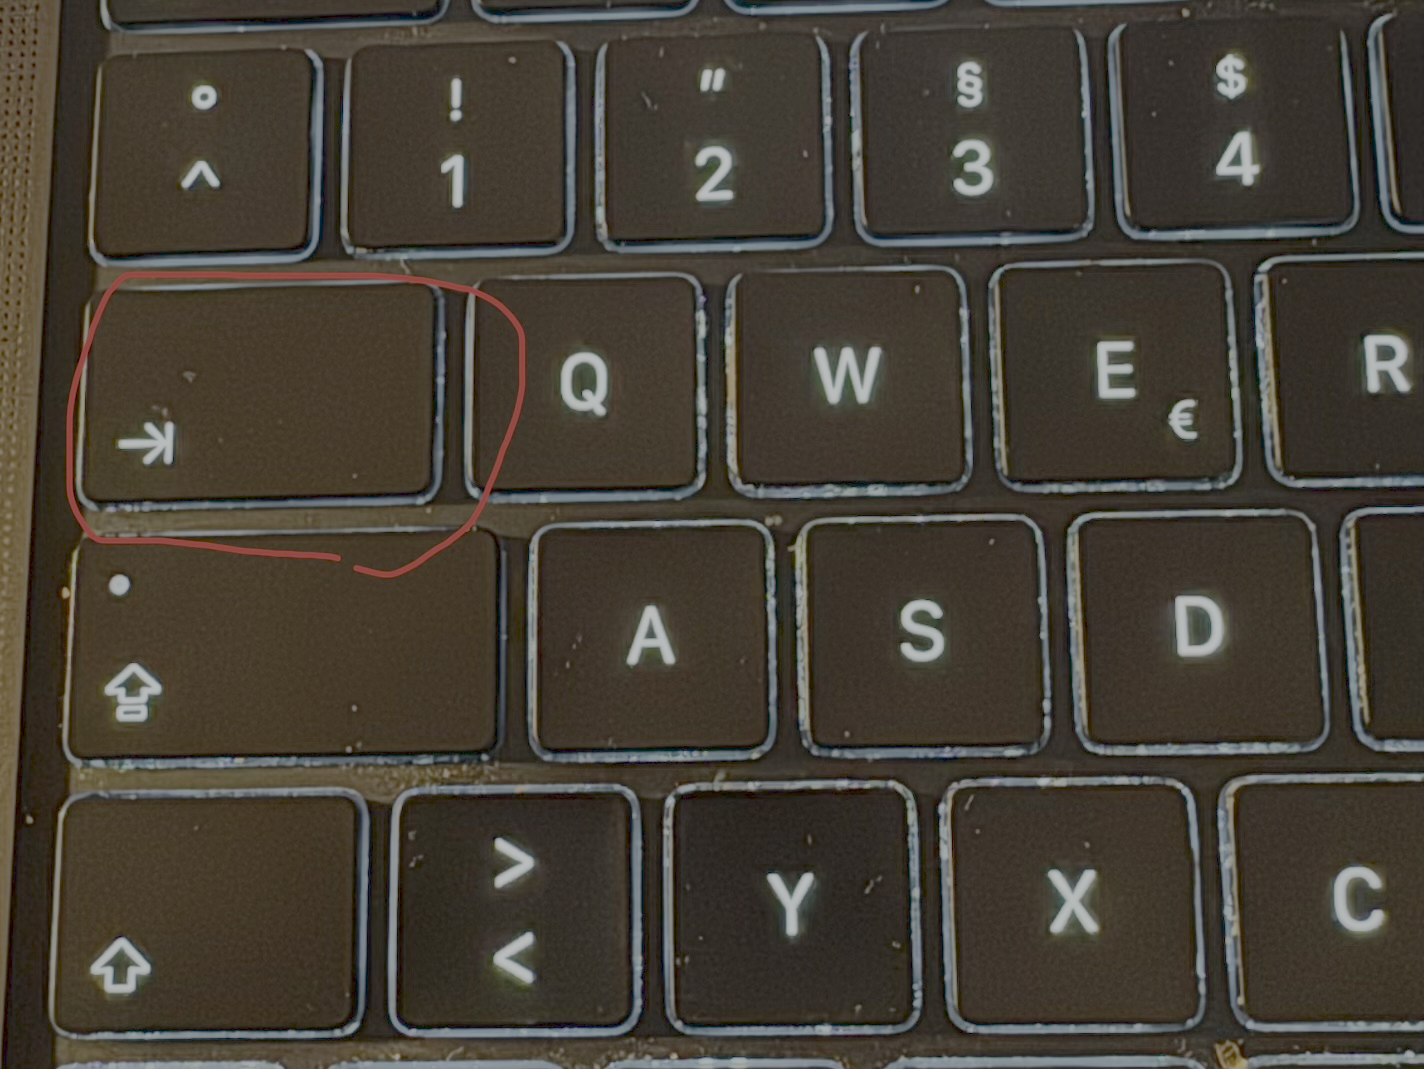
\includegraphics[keepaspectratio]{images/tabulatortaste.png}}
\end{frame}

\section{Sitzung 4: Deskriptive Statistik \& Datentransformation
II}\label{sitzung-4-deskriptive-statistik-datentransformation-ii}

\begin{frame}{Logistik}
\protect\phantomsection\label{logistik-1}
\begin{itemize}
\tightlist
\item
  Nächste Woche nur 1. Session
\end{itemize}
\end{frame}

\begin{frame}{Lernziele dieser Sitzung}
\protect\phantomsection\label{lernziele-dieser-sitzung-2}
\begin{itemize}
\tightlist
\item
  Datensätze mit Joins verknüpfen
\item
  Typische Datenfehler erkennen und beheben
\item
  Lagemaße berechnen und interpretieren
\item
  Den Unterschied zwischen Mittelwert und Median erklären
\item
  Verteilungen anhand von Histogramm und Streudiagramm beurteilen
\end{itemize}
\end{frame}

\begin{frame}{Typischer Ablauf einer Analyse}
\protect\phantomsection\label{typischer-ablauf-einer-analyse}
\pandocbounded{\includegraphics[keepaspectratio]{images/CRISP-DM_Process_Diagram.png}}
\end{frame}

\begin{frame}{Typische Fehler}
\protect\phantomsection\label{typische-fehler}
\begin{itemize}
\tightlist
\item
  Package nicht geladen
\item
  Pipe-Symbol falsch verwendet
\item
  Unvollständige Code-Chunks
\end{itemize}
\end{frame}

\begin{frame}{Wir starten mit einer Übung}
\protect\phantomsection\label{wir-starten-mit-einer-uxfcbung}
\begin{itemize}
\tightlist
\item
  Importieren Sie die beiden anderen Bücher-Datensätze
\item
  Achten Sie auf die richtigen Datentypen beim Import
\item
  Fällt Ihnen was auf bei den Altersangaben der Nutzer?
\item
  Überlegen Sie, was die verbindenden Spalten sind, mit denen die
  Datensätze miteiner verbunden werden könnten
\end{itemize}
\end{frame}

\begin{frame}{Irgendwas stimmt mit dem Alter nicht}
\protect\phantomsection\label{irgendwas-stimmt-mit-dem-alter-nicht}
\begin{itemize}
\tightlist
\item
  Vieles wird schneller klar, wenn die Daten visualisiert werden
\item
  Tatsächlich visualisieren wir Daten immer gleich zu Beginn
\item
  Welche Visualisierung kennen Sie bereits?
\end{itemize}
\end{frame}

\begin{frame}{Demo}
\protect\phantomsection\label{demo}
\begin{itemize}
\tightlist
\item
  Histogram mit ggplot
\end{itemize}
\end{frame}

\begin{frame}{Histogramm}
\protect\phantomsection\label{histogramm}
\begin{itemize}
\tightlist
\item
  Was: Grafische Darstellung der Häufigkeitsverteilung in Klassen
\item
  Bestandteile: X-Achse (Werte), Y-Achse (Häufigkeit), Balken
  (Klassenhäufigkeit)
\item
  Wozu: Schneller Überblick über Datenverteilung und -muster
\item
  Interpretation: Form (symmetrisch/schief), Modalität
  (uni-/multimodal), Ausreißer
\item
  Wichtig: Klassenanzahl beeinflusst sichtbare Form
\end{itemize}
\end{frame}

\begin{frame}{Let's talk about money}
\protect\phantomsection\label{lets-talk-about-money}
\pandocbounded{\includegraphics[keepaspectratio]{images/einkommen.jpeg}}
\end{frame}

\begin{frame}{Wie könnte man die Einkommensverteilung beschreiben?}
\protect\phantomsection\label{wie-kuxf6nnte-man-die-einkommensverteilung-beschreiben}
\pandocbounded{\includegraphics[keepaspectratio]{images/einkommensschichtung.png}}
\#\# Im Durchschnitt haben Sie\ldots{}

\begin{columns}[T]
\begin{column}{0.5\linewidth}
\pandocbounded{\includegraphics[keepaspectratio]{images/schulden1.png}}
\end{column}

\begin{column}{0.5\linewidth}
\pandocbounded{\includegraphics[keepaspectratio]{images/schulden2.png}}
\end{column}
\end{columns}
\end{frame}

\begin{frame}{Warum sind statistische Kennzahlen wichtig?}
\protect\phantomsection\label{warum-sind-statistische-kennzahlen-wichtig}
\begin{itemize}
\tightlist
\item
  \textbf{Reduktion von Komplexität}: Große Datenmengen werden durch
  wenige Werte beschreibbar
\item
  \textbf{Kommunikation}: Leichtere Vermittlung von Erkenntnissen an
  Nicht-Statistiker
\item
  \textbf{Vergleichbarkeit}: Unterschiedliche Datensätze werden
  vergleichbar
\end{itemize}
\end{frame}

\begin{frame}{Typische Anwendungsfälle}
\protect\phantomsection\label{typische-anwendungsfuxe4lle}
{\def\LTcaptype{none} % do not increment counter
\begin{longtable}[]{@{}
  >{\raggedright\arraybackslash}p{(\linewidth - 4\tabcolsep) * \real{0.3333}}
  >{\raggedright\arraybackslash}p{(\linewidth - 4\tabcolsep) * \real{0.3333}}
  >{\raggedright\arraybackslash}p{(\linewidth - 4\tabcolsep) * \real{0.3333}}@{}}
\toprule\noalign{}
\begin{minipage}[b]{\linewidth}\raggedright
Kennzahl
\end{minipage} & \begin{minipage}[b]{\linewidth}\raggedright
Wichtig für\ldots{}
\end{minipage} & \begin{minipage}[b]{\linewidth}\raggedright
Beispielanwendung
\end{minipage} \\
\midrule\noalign{}
\endhead
\textbf{Mittelwert} & Durchschnittswerte, Summenbetrachtungen &
Durchschnittseinkommen einer Region \\
\textbf{Median} & Typische Werte, robust gegen Ausreißer & Typisches
Haushaltseinkommen \\
\textbf{Standardabweichung} & Streuung, Qualitätskontrolle &
Produktionsgenauigkeit in der Fertigung \\
\textbf{Quartile/Boxplot} & Verteilungsform, Ausreißererkennung &
Identifikation von Ungleichheiten \\
\textbf{Schiefe/Wölbung} & Abweichungen von der Normalverteilung &
Risikobewertung im Finanzwesen \\
\bottomrule\noalign{}
\end{longtable}
}
\end{frame}

\begin{frame}{Von der Beschreibung zur Inferenz}
\protect\phantomsection\label{von-der-beschreibung-zur-inferenz}
\begin{itemize}
\tightlist
\item
  Deskriptive Statistik als Grundlage für \textbf{statistische Tests}
\item
  Möglichkeit der \textbf{Stichprobenerhebung} statt Vollerhebung
\item
  Basis für \textbf{statistische Modellierung} und \textbf{Vorhersagen}
\end{itemize}
\end{frame}

\begin{frame}{Erkennung von Mustern und Besonderheiten}
\protect\phantomsection\label{erkennung-von-mustern-und-besonderheiten}
\begin{itemize}
\tightlist
\item
  \textbf{Ausreißer}: Potentielle Fehler oder besondere Fälle
\item
  \textbf{Trends}: Entwicklungen über Zeit
\item
  \textbf{Gruppenunterschiede}: Systematische Variation zwischen
  Teilgruppen
\end{itemize}
\end{frame}

\begin{frame}{Weitere Beispiele}
\protect\phantomsection\label{weitere-beispiele}
{\def\LTcaptype{none} % do not increment counter
\begin{longtable}[]{@{}
  >{\raggedright\arraybackslash}p{(\linewidth - 4\tabcolsep) * \real{0.3333}}
  >{\raggedright\arraybackslash}p{(\linewidth - 4\tabcolsep) * \real{0.3333}}
  >{\raggedright\arraybackslash}p{(\linewidth - 4\tabcolsep) * \real{0.3333}}@{}}
\toprule\noalign{}
\begin{minipage}[b]{\linewidth}\raggedright
Anwendungsgebiet
\end{minipage} & \begin{minipage}[b]{\linewidth}\raggedright
Kennzahlen
\end{minipage} & \begin{minipage}[b]{\linewidth}\raggedright
Nutzen
\end{minipage} \\
\midrule\noalign{}
\endhead
\textbf{Medizin} & Referenzwerte (z.B. Blutdruck, BMI) & Diagnostik,
Risikoeinschätzung \\
\textbf{Finanzmarkt} & Volatilität (Standardabweichung) &
Risikobewertung von Anlagen \\
\textbf{Qualitätssicherung} & Prozessfähigkeitsindizes (basierend auf σ)
& Optimierung von Produktionsprozessen \\
\textbf{Sozialforschung} & Gini-Koeffizient (basierend auf Verteilung) &
Ungleichheitsmaße in der Gesellschaft \\
\textbf{Meteorologie} & Durchschnittstemperaturen + Extremwerte &
Klimaforschung, Wettervorhersage \\
\bottomrule\noalign{}
\end{longtable}
}
\end{frame}

\begin{frame}{Lagemaße}
\protect\phantomsection\label{lagemauxdfe}
\pandocbounded{\includegraphics[keepaspectratio]{images/mean-mode-median.png}}
\end{frame}

\begin{frame}{Lagemaße}
\protect\phantomsection\label{lagemauxdfe-1}
\begin{itemize}
\tightlist
\item
  Mean bezeichnet das arithmetische Mittel, häufig als „Durchschnitt''
  bezeichnet: mean()
\item
  Neben dem arithmetischen Mittel existieren weitere Mittelwerte, zum
  Beispiel das geometrische Mittel
\item
  Der Median ist weniger anfällig für Ausreißer: median()
\item
  Der Modalwert kann auch mit kategorialen Variablen umgehen
\item
  In R existiert kein Befehl für den Modalwert ☹
\end{itemize}
\end{frame}

\begin{frame}{Merke}
\protect\phantomsection\label{merke}
\pandocbounded{\includegraphics[keepaspectratio]{images/meme-durchschnitt.png}}
\end{frame}

\begin{frame}{It really happened}
\protect\phantomsection\label{it-really-happened}
\pandocbounded{\includegraphics[keepaspectratio]{images/clinton-average.png}}
\end{frame}

\begin{frame}{Auch die MOPO\ldots{}}
\protect\phantomsection\label{auch-die-mopo}
\pandocbounded{\includegraphics[keepaspectratio]{images/Bildschirmfoto 2025-05-09 um 11.34.35.png}}
\end{frame}

\begin{frame}{Typisch / ungewöhnlich / unmöglich}
\protect\phantomsection\label{typisch-ungewuxf6hnlich-unmuxf6glich}
\pandocbounded{\includegraphics[keepaspectratio]{images/hadlum.png}}
\end{frame}

\begin{frame}{Warum Visualisierung auch wichtig ist}
\protect\phantomsection\label{warum-visualisierung-auch-wichtig-ist}
\pandocbounded{\includegraphics[keepaspectratio]{images/Anscombe's_quartet_3.svg.png}}
\end{frame}

\begin{frame}{Formparameter}
\protect\phantomsection\label{formparameter}
\pandocbounded{\includegraphics[keepaspectratio]{images/3-s2.0-B9780128207178000087-f05-03-9780128207178.jpg}}
\end{frame}

\begin{frame}[fragile]{Schiefe (Skewness)}
\protect\phantomsection\label{schiefe-skewness}
\begin{itemize}
\tightlist
\item
  Misst die Asymmetrie einer Verteilung
\item
  Positive Schiefe: rechtsschiefe Verteilung (längerer ``Schwanz'' nach
  rechts)
\item
  Negative Schiefe: linksschiefe Verteilung (längerer ``Schwanz'' nach
  links)
\item
  Schiefe von 0: symmetrische Verteilung (z.B. Normalverteilung)
\item
  In R: \texttt{skewness(data)} aus dem Paket \textbf{moments} oder
  \textbf{e1071}
\end{itemize}
\end{frame}

\begin{frame}[fragile]{Wölbung (Kurtosis)}
\protect\phantomsection\label{wuxf6lbung-kurtosis}
\begin{itemize}
\tightlist
\item
  Misst die ``Spitzheit'' bzw. ``Flachheit'' einer Verteilung
\item
  Normalverteilung hat eine Kurtosis von 3 (manchmal als Exzess-Kurtosis
  = 0 dargestellt)
\item
  Hohe Kurtosis (\textgreater3): spitze Verteilung mit ``schweren
  Enden'' (mehr Extremwerte)
\item
  Niedrige Kurtosis (\textless3): flache Verteilung mit ``leichten
  Enden'' (weniger Extremwerte)
\item
  In R: \texttt{kurtosis(data)} aus dem Paket \textbf{moments} oder
  \textbf{e1071}
\end{itemize}
\end{frame}

\begin{frame}[fragile]{Weitere Positionskennwerte: Quantile und
Perzentile}
\protect\phantomsection\label{weitere-positionskennwerte-quantile-und-perzentile}
\begin{itemize}
\tightlist
\item
  Teile die Daten in gleich große Teile
\item
  Median = 0,5-Quantil (50\%-Perzentil)
\item
  Quartile teilen die Daten in vier gleiche Teile:

  \begin{itemize}
  \tightlist
  \item
    Q1 = 0,25-Quantil (25\%-Perzentil)
  \item
    Q2 = 0,5-Quantil (50\%-Perzentil) = Median
  \item
    Q3 = 0,75-Quantil (75\%-Perzentil)
  \end{itemize}
\item
  In R: \texttt{quantile(data,\ probs\ =\ c(0.25,\ 0.5,\ 0.75))} für
  Quartile
\end{itemize}
\end{frame}

\begin{frame}{Datensätze miteinander verbinden}
\protect\phantomsection\label{datensuxe4tze-miteinander-verbinden}
\pandocbounded{\includegraphics[keepaspectratio]{images/joins.png}}
\end{frame}

\section{Sitzung 5}\label{sitzung-5}

\begin{frame}{Streuungsmaße}
\protect\phantomsection\label{streuungsmauxdfe}
\end{frame}

\begin{frame}[fragile]{Spannweite (Range)}
\protect\phantomsection\label{spannweite-range}
\begin{itemize}
\tightlist
\item
  Die Spannweite ist der einfachste Streuungsparameter
\item
  Berechnung: Maximum - Minimum
\item
  Sehr anfällig für Ausreißer
\item
  In R: \texttt{diff(range(data))} oder \texttt{max(data)\ -\ min(data)}
\end{itemize}
\end{frame}

\begin{frame}[fragile]{Interquartilsabstand (IQR)}
\protect\phantomsection\label{interquartilsabstand-iqr}
\begin{itemize}
\tightlist
\item
  Robusteres Streuungsmaß, das Ausreißer besser berücksichtigt
\item
  Berechnung: 75\%-Quartil minus 25\%-Quartil (Q3 - Q1)
\item
  Enthält die mittleren 50\% der Daten
\item
  In R: \texttt{IQR(data)} oder
  \texttt{quantile(data,\ 0.75)\ -\ quantile(data,\ 0.25)}
\end{itemize}
\end{frame}

\begin{frame}[fragile]{Varianz}
\protect\phantomsection\label{varianz}
\begin{itemize}
\tightlist
\item
  Durchschnittliche quadratische Abweichung vom Mittelwert
\item
  Berechnung für Grundgesamtheit:
  \[\sigma^2 = \frac{1}{N} \sum_{i=1}^{N} (x_i - \mu)^2\]
\item
  Berechnung für Stichprobe (korrigierte Varianz):
  \[s^2 = \frac{1}{n-1} \sum_{i=1}^{n} (x_i - \bar{x})^2\]
\item
  Einheit: Quadrat der Einheit der Ursprungsdaten
\item
  In R: \texttt{var(data)}
\end{itemize}
\end{frame}

\begin{frame}{Standardabweichung}
\protect\phantomsection\label{standardabweichung}
\pandocbounded{\includegraphics[keepaspectratio]{images/Standard_deviation_diagram.svg.png}}
\end{frame}

\begin{frame}[fragile]{Standardabweichung}
\protect\phantomsection\label{standardabweichung-1}
\begin{itemize}
\tightlist
\item
  Wurzel aus der Varianz: Dieselbe Einheit wie die Ursprungsdaten
\item
  Berechnung für Grundgesamtheit:
  \[\sigma = \sqrt{\frac{1}{N} \sum_{i=1}^{N} (x_i - \mu)^2}\]
\item
  Berechnung für Stichprobe:
  \[s = \sqrt{\frac{1}{n-1} \sum_{i=1}^{n} (x_i - \bar{x})^2}\]
\item
  In R: \texttt{sd(data)}
\end{itemize}
\end{frame}

\begin{frame}{Interpretation der Standardabweichung im Kontext der
Normalverteilung}
\protect\phantomsection\label{interpretation-der-standardabweichung-im-kontext-der-normalverteilung}
\begin{itemize}
\tightlist
\item
  Bei normalverteilten Daten liegen ca. 68\% der Werte innerhalb von μ ±
  σ (Mittelwert ± 1 Standardabweichung)
\item
  Ca. 95\% der Werte liegen innerhalb von μ ± 2σ
\item
  Ca. 99,7\% der Werte liegen innerhalb von μ ± 3σ
  (``Drei-Sigma-Regel'')
\end{itemize}
\end{frame}

\begin{frame}{Boxplot}
\protect\phantomsection\label{boxplot}
\pandocbounded{\includegraphics[keepaspectratio]{images/Elements_of_a_boxplot.svg.png}}
\end{frame}

\begin{frame}[fragile]{Boxplot}
\protect\phantomsection\label{boxplot-1}
\begin{itemize}
\tightlist
\item
  Visuelle Darstellung von Quartilen und Ausreißern
\item
  Box: Interquartilsabstand (IQR) von Q1 bis Q3
\item
  Mittellinie: Median (Q2)
\item
  Whiskers: Typischerweise bis max. 1,5 × IQR von der Box
\item
  Punkte außerhalb der Whiskers: potenzielle Ausreißer
\item
  In R: \texttt{boxplot(data)}
\end{itemize}

\pandocbounded{\includegraphics[keepaspectratio]{images/Elements_of_a_boxplot.svg.png}}
\end{frame}

\begin{frame}[fragile]{Wie macht man das in R?}
\protect\phantomsection\label{wie-macht-man-das-in-r}
{\def\LTcaptype{none} % do not increment counter
\begin{longtable}[]{@{}
  >{\raggedright\arraybackslash}p{(\linewidth - 4\tabcolsep) * \real{0.3333}}
  >{\raggedright\arraybackslash}p{(\linewidth - 4\tabcolsep) * \real{0.3333}}
  >{\raggedright\arraybackslash}p{(\linewidth - 4\tabcolsep) * \real{0.3333}}@{}}
\toprule\noalign{}
\begin{minipage}[b]{\linewidth}\raggedright
Kennzahl
\end{minipage} & \begin{minipage}[b]{\linewidth}\raggedright
R‑Befehl
\end{minipage} & \begin{minipage}[b]{\linewidth}\raggedright
Kurzbeschreibung
\end{minipage} \\
\midrule\noalign{}
\endhead
Mittelwert & \texttt{mean(data)} & Durchschnitt aller Werte \\
Median & \texttt{median(data)} & Zentralwert (50 \%-Quantil) \\
Minimum & \texttt{min(data)} & Kleinster Wert \\
Maximum & \texttt{max(data)} & Größter Wert \\
Spannweite & \texttt{diff(range(data))} & Abstand = Max − Min \\
Standardabweichung & \texttt{sd(data)} & Ø‑Abweichung vom Mittelwert \\
Varianz & \texttt{var(data)} & Quadrat der Standardabweichung \\
Schiefe & \texttt{skewness(data)} \emph{(moments/e1071)} & Asymmetrie
der Verteilung \\
Wölbung (Kurtosis) & \texttt{kurtosis(data)} \emph{(moments/e1071)} &
``Spitzheit'' der Verteilung \\
Quantile & \texttt{quantile(data,\ c(.25,.5,.75))} & 25 \%, 50 \%, 75
\%-Werte (Quartile) \\
\bottomrule\noalign{}
\end{longtable}
}
\end{frame}

\begin{frame}[fragile]{Übung mit dem Datensatz iris}
\protect\phantomsection\label{uxfcbung-mit-dem-datensatz-iris}
{\def\LTcaptype{none} % do not increment counter
\begin{longtable}[]{@{}
  >{\raggedright\arraybackslash}p{(\linewidth - 4\tabcolsep) * \real{0.2740}}
  >{\raggedright\arraybackslash}p{(\linewidth - 4\tabcolsep) * \real{0.2877}}
  >{\raggedright\arraybackslash}p{(\linewidth - 4\tabcolsep) * \real{0.4384}}@{}}
\toprule\noalign{}
\begin{minipage}[b]{\linewidth}\raggedright
Kennzahl
\end{minipage} & \begin{minipage}[b]{\linewidth}\raggedright
R‑Befehl
\end{minipage} & \begin{minipage}[b]{\linewidth}\raggedright
Kurzbeschreibung
\end{minipage} \\
\midrule\noalign{}
\endhead
Mittelwert & \texttt{mean(data)} & Durchschnitt aller Werte \\
Median & \texttt{median(data)} & Zentralwert (50 \%-Quantil) \\
Minimum & \texttt{min(data)} & Kleinster Wert \\
Maximum & \texttt{max(data)} & Größter Wert \\
Spannweite & \texttt{diff(range(data))} & Abstand = Max − Min \\
Standardabweichung & \texttt{sd(data)} & Ø‑Abweichung vom Mittelwert \\
Varianz & \texttt{var(data)} & Quadrat der Standardabweichung \\
\bottomrule\noalign{}
\end{longtable}
}
\end{frame}

\begin{frame}{Demo}
\protect\phantomsection\label{demo-1}
\end{frame}

\section{Sitzung 5:
Datenvisualisierung}\label{sitzung-5-datenvisualisierung}

\begin{frame}{Lernziele dieser Sitzung}
\protect\phantomsection\label{lernziele-dieser-sitzung-3}
\begin{itemize}
\tightlist
\item
  Das richtige Diagramm für eine Fragestellung auswählen
\item
  Grundprinzipien guter Visualisierung anwenden (Clutter, Highlighting,
  Storytelling)
\item
  Diagramme mit ggplot2 erstellen
\item
  Häufige Fehler bei der Datenvisualisierung vermeiden
\end{itemize}
\end{frame}

\begin{frame}{Warum Datenvisualisierung?}
\protect\phantomsection\label{warum-datenvisualisierung}
The greatest value of a picture is when it forces us to notice what we
never expected to see. (John Tukey)
\end{frame}

\begin{frame}{Warum Datenvisualisierung, Teil 2}
\protect\phantomsection\label{warum-datenvisualisierung-teil-2}
\pandocbounded{\includegraphics[keepaspectratio]{images/Anscombe's_quartet_3.svg.png}}
\end{frame}

\begin{frame}{5 wichtige Schritte}
\protect\phantomsection\label{wichtige-schritte}
\begin{enumerate}
\tightlist
\item
  Was ist der Kontext?

  \begin{itemize}
  \tightlist
  \item
    An wen wird kommuniziert?
  \item
    Was soll der Empfänger wissen oder tun?
  \item
    Welche Daten sind vorhanden, um den Case zu untermauern?
  \end{itemize}
\end{enumerate}
\end{frame}

\begin{frame}{5 wichtige Schritte}
\protect\phantomsection\label{wichtige-schritte-1}
\begin{enumerate}
\setcounter{enumi}{1}
\tightlist
\item
  Welche ist das passendste Visualierung?

  \begin{itemize}
  \tightlist
  \item
    Ein oder zwei Zahlen, die im Fokus stehen? =\textgreater{} Text!
  \item
    Liniendiagramme für continuous data
  \item
    Säulendiagramme für kategoriale Daten, müssen bei 0 anfangen
  \item
    Die Beziehungen der Daten untereinander bestimmen die
    Visualisierung, sofern Sie mehr als eine Variable haben
  \item
    Vermeiden Sie Tortendiagramme, Donuts, 3D, zweite Y-Achsen
  \end{itemize}
\end{enumerate}
\end{frame}

\begin{frame}{5 wichtige Schritte}
\protect\phantomsection\label{wichtige-schritte-2}
\begin{enumerate}
\setcounter{enumi}{2}
\tightlist
\item
  Entfernen Sie „Clutter''

  \begin{enumerate}
  \tightlist
  \item
    Entfernen Sie alles, das keinen informativen Mehrwert hat (z.B.
    Farben für die Ästhetik)
  \item
    Arbeiten Sie mit freiem Raum
  \end{enumerate}
\end{enumerate}
\end{frame}

\begin{frame}{5 wichtige Schritte}
\protect\phantomsection\label{wichtige-schritte-3}
\begin{enumerate}
\setcounter{enumi}{3}
\tightlist
\item
  Fokussieren Sie die Aufmerksamkeit, wo Sie hin soll

  \begin{itemize}
  \tightlist
  \item
    Größe, Position und, ja, manchmal auch Farbe nutzen um zu
    signalisieren, was wichtig ist
  \item
    Wohin gehen die Augen?
  \end{itemize}
\end{enumerate}
\end{frame}

\begin{frame}{5 wichtige Schritte}
\protect\phantomsection\label{wichtige-schritte-4}
\begin{columns}[T]
\begin{column}{0.6\linewidth}
\begin{enumerate}
\setcounter{enumi}{4}
\tightlist
\item
  Nutzen Sie Storytelling

  \begin{itemize}
  \tightlist
  \item
    Niemand will einfach nur Auflistungen von Zahlen und Diagrammen
    sehen.
  \item
    Schreiben Sie einen Plot. Anfang, eventuell sogar einen Twist, und
    ein Ende mit Call to Action (in der Wissenschaft reicht eine
    Diskussion ☺)
  \item
    Bitte arbeiten Sie nicht einfach nur mechanisch alles ab, was Sie
    können.
  \end{itemize}
\end{enumerate}
\end{column}

\begin{column}{0.4\linewidth}
\pandocbounded{\includegraphics[keepaspectratio]{images/storytelling.png}}
\end{column}
\end{columns}
\end{frame}

\begin{frame}{Redundant Coding}
\protect\phantomsection\label{redundant-coding}
\begin{columns}[T]
\begin{column}{0.5\linewidth}
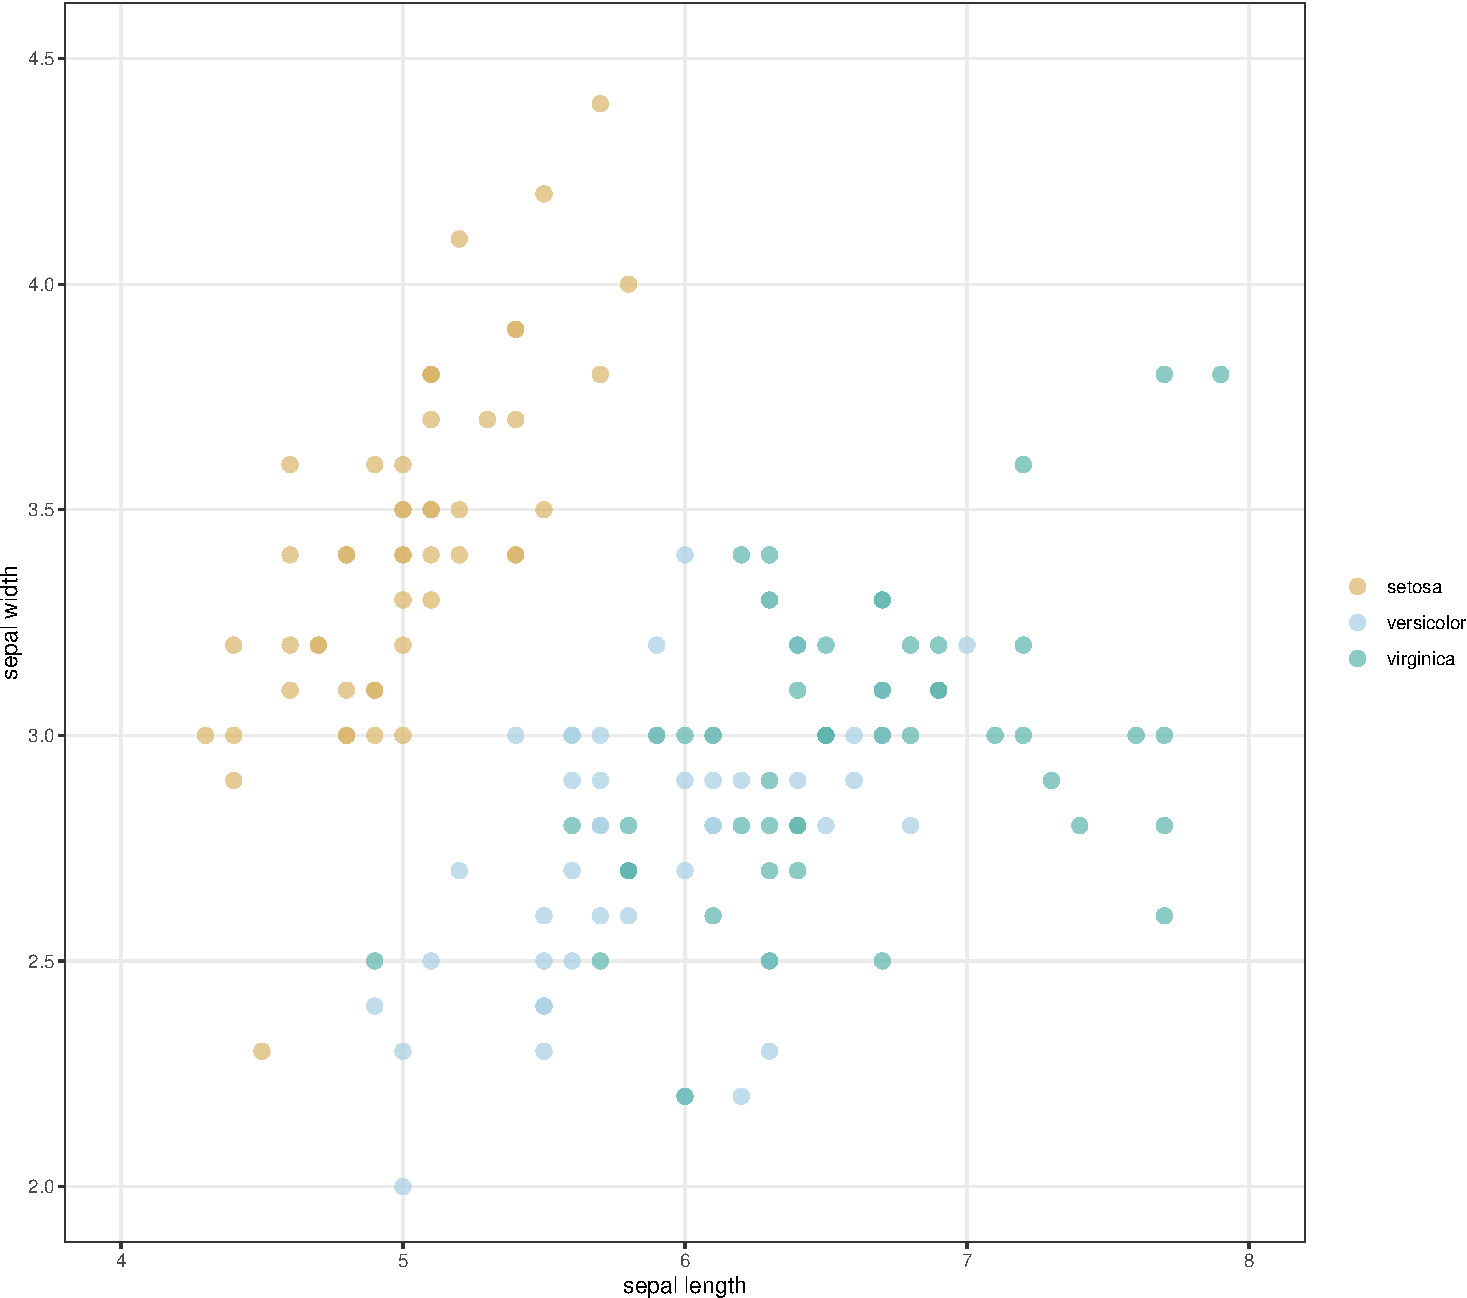
\includegraphics[width=1\linewidth,height=\textheight,keepaspectratio]{Statistik_Seminar_files/figure-beamer/unnamed-chunk-2-1.pdf}
\end{column}

\begin{column}{0.5\linewidth}
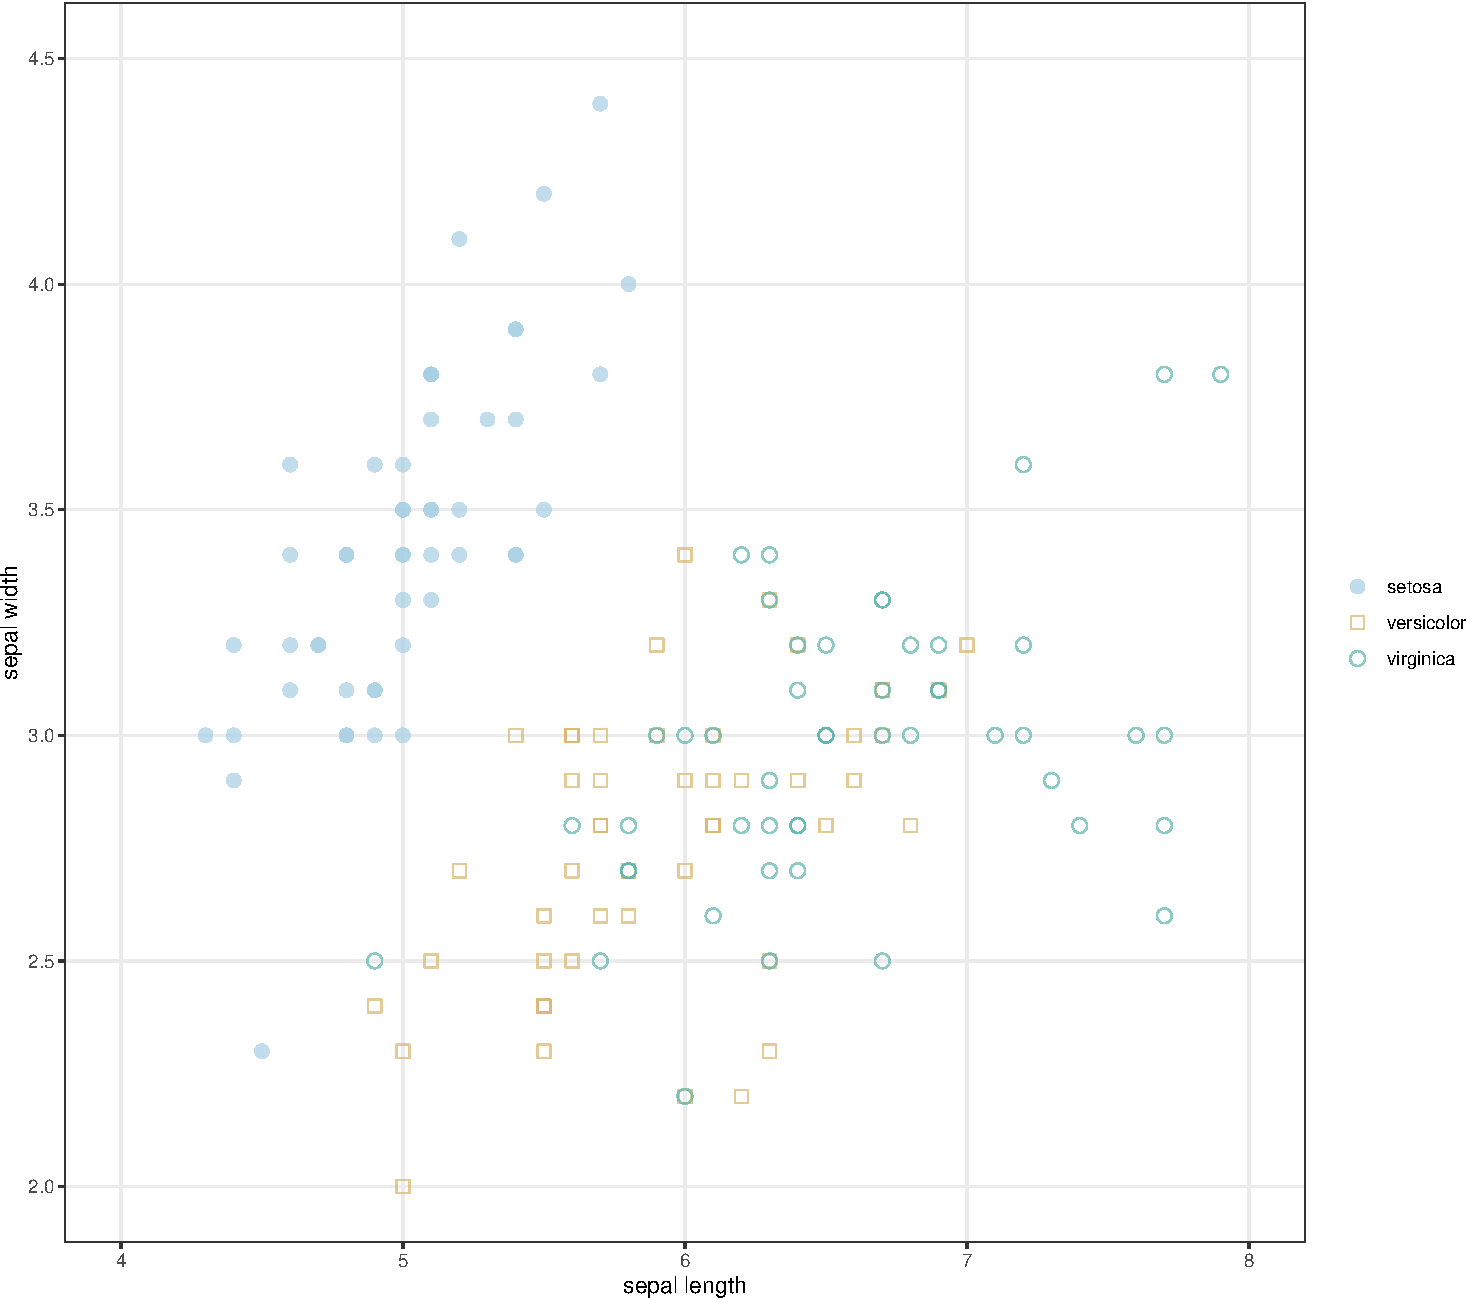
\includegraphics[width=1\linewidth,height=\textheight,keepaspectratio]{Statistik_Seminar_files/figure-beamer/unnamed-chunk-3-1.pdf}
\end{column}
\end{columns}
\end{frame}

\begin{frame}{Weißer Space ist gut\ldots{} aber nicht zu viel!}
\protect\phantomsection\label{weiuxdfer-space-ist-gut-aber-nicht-zu-viel}
\begin{columns}[T]
\begin{column}{0.5\linewidth}
\pandocbounded{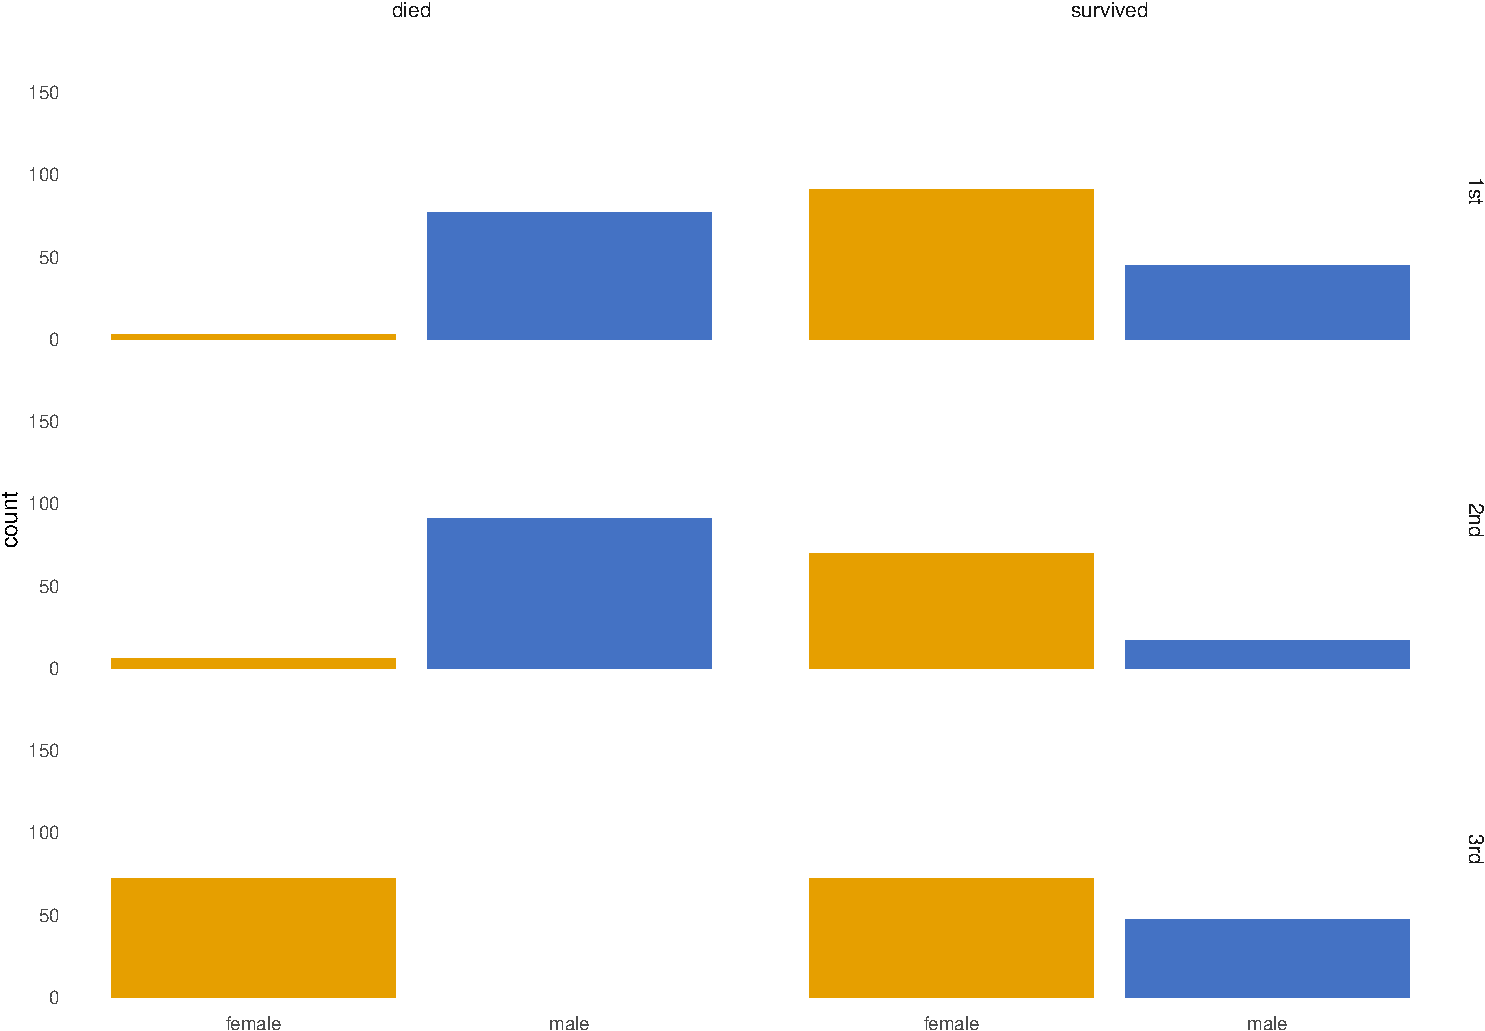
\includegraphics[keepaspectratio]{Statistik_Seminar_files/figure-beamer/unnamed-chunk-4-1.pdf}}
\end{column}

\begin{column}{0.5\linewidth}
\pandocbounded{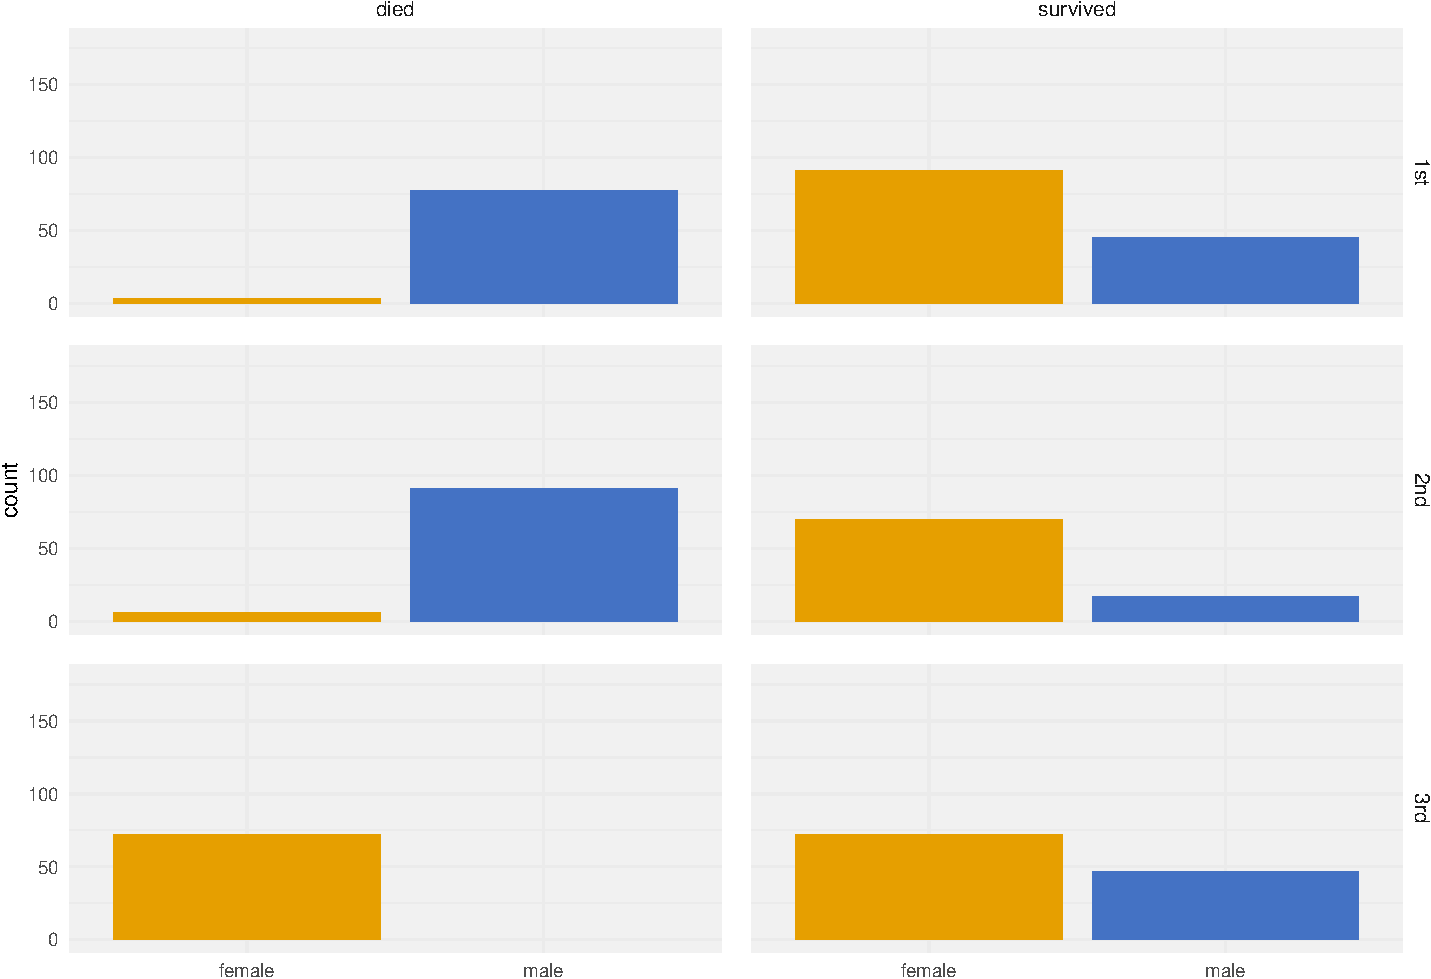
\includegraphics[keepaspectratio]{Statistik_Seminar_files/figure-beamer/unnamed-chunk-5-1.pdf}}
\end{column}
\end{columns}
\end{frame}

\begin{frame}{Highlighting}
\protect\phantomsection\label{highlighting}
\pandocbounded{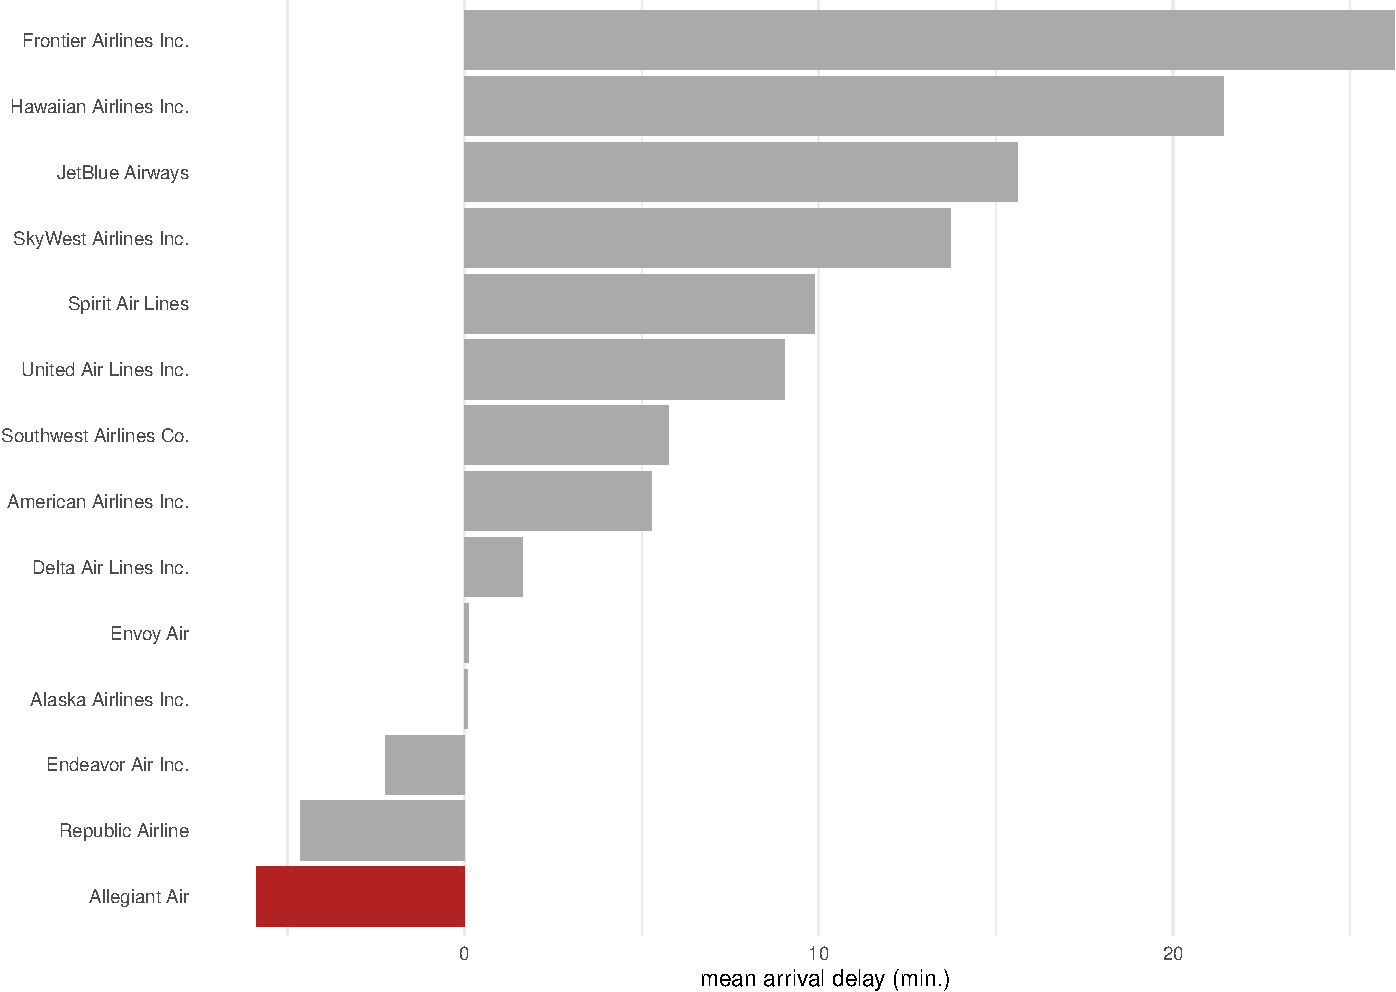
\includegraphics[keepaspectratio]{Statistik_Seminar_files/figure-beamer/unnamed-chunk-6-1.pdf}}
\end{frame}

\begin{frame}{Wie identifiziert man das richtige Diagramm?}
\protect\phantomsection\label{wie-identifiziert-man-das-richtige-diagramm}
\pandocbounded{\includegraphics[keepaspectratio]{images/overview.png}}
\end{frame}

\begin{frame}{Scatter Plot / Streudiagramm}
\protect\phantomsection\label{scatter-plot-streudiagramm}
\begin{columns}[T]
\begin{column}{0.6\linewidth}
\begin{itemize}
\tightlist
\item
  Zeigt Beziehung zwischen zwei kontinuierlichen Variablen
\item
  Jeder Punkt = eine Beobachtung
\item
  Erkennt Muster, Cluster, Ausreißer und Korrelationen
\item
  Benötigt numerische X/Y-Achsen
\item
  Dritte Dimension durch Punktgröße/Farbe möglich
\end{itemize}
\end{column}

\begin{column}{0.4\linewidth}
\pandocbounded{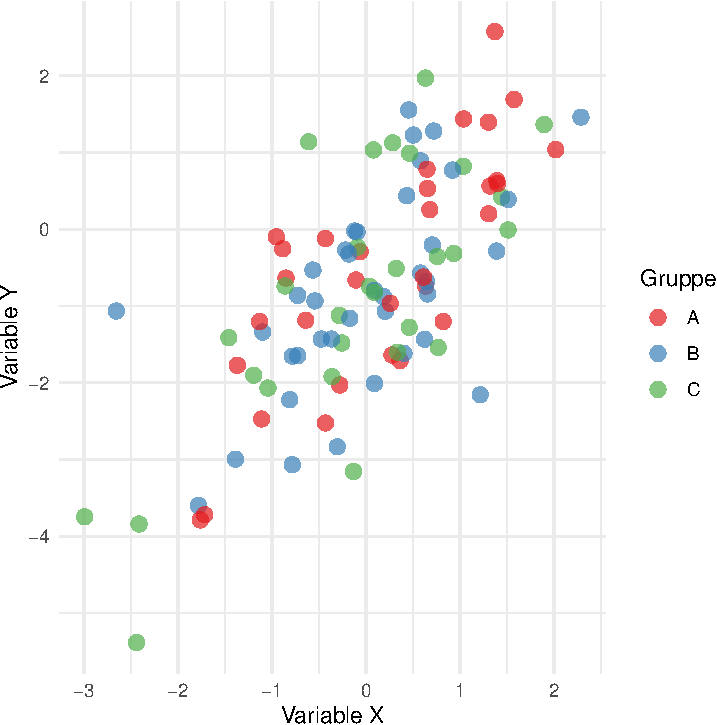
\includegraphics[keepaspectratio]{Statistik_Seminar_files/figure-beamer/unnamed-chunk-7-1.pdf}}
\end{column}
\end{columns}
\end{frame}

\begin{frame}{Korrelationsmatrix}
\protect\phantomsection\label{korrelationsmatrix}
\begin{columns}[T]
\begin{column}{0.6\linewidth}
\begin{itemize}
\tightlist
\item
  Zeigt Korrelationsstärke zwischen Variablen
\item
  Farbe/Größe visualisiert Richtung und Stärke
\item
  Unterscheidet klar positive/negative Korrelationen
\item
  Identifiziert Muster und redundante Variablen
\item
  Essentiell für explorative Datenanalyse
\end{itemize}
\end{column}

\begin{column}{0.4\linewidth}
\pandocbounded{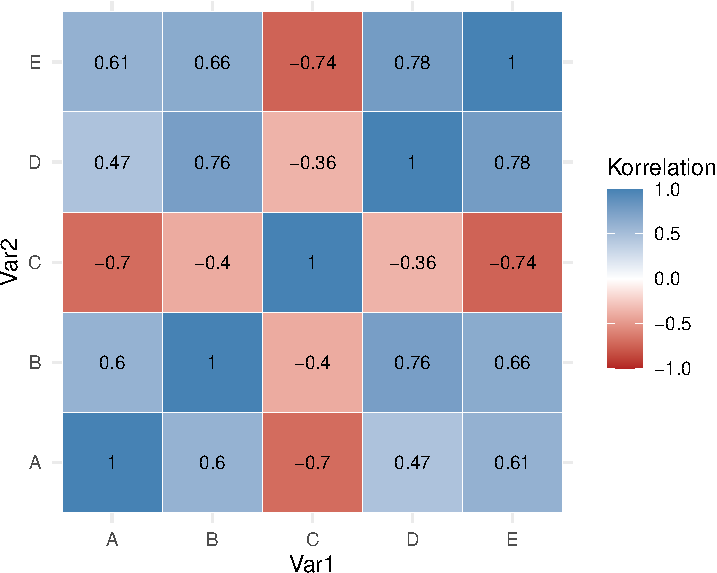
\includegraphics[keepaspectratio]{Statistik_Seminar_files/figure-beamer/unnamed-chunk-8-1.pdf}}
\end{column}
\end{columns}
\end{frame}

\begin{frame}{Venn-Diagramm}
\protect\phantomsection\label{venn-diagramm}
\begin{columns}[T]
\begin{column}{0.6\linewidth}
\begin{itemize}
\tightlist
\item
  Zeigt gemeinsame und einzigartige Elemente
\item
  Überschneidungen visualisieren Gemeinsamkeiten
\item
  Ideal für Vergleich von Kategorien/Merkmalen
\item
  Funktioniert am besten mit 2-3 Gruppen
\item
  Wird mit mehr als 5 Gruppen unübersichtlich
\end{itemize}
\end{column}

\begin{column}{0.4\linewidth}
\pandocbounded{\includegraphics[keepaspectratio]{images/relationship_venn_4_3.png}}
\end{column}
\end{columns}
\end{frame}

\begin{frame}{UpSet Diagram}
\protect\phantomsection\label{upset-diagram}
\begin{columns}[T]
\begin{column}{0.6\linewidth}
\begin{itemize}
\tightlist
\item
  Alternative für komplexe Überschneidungen
\item
  Skalierbarer als klassische Venn-Diagramme
\item
  Balken visualisieren Überschneidungsgrößen
\item
  Punkte zeigen beteiligte Mengen
\item
  Ideal für 4+ Gruppen/komplexe Beziehungen
\end{itemize}
\end{column}

\begin{column}{0.4\linewidth}
\pandocbounded{\includegraphics[keepaspectratio]{images/upset.png}}
\end{column}
\end{columns}
\end{frame}

\begin{frame}{Sankey Diagram}
\protect\phantomsection\label{sankey-diagram}
\begin{columns}[T]
\begin{column}{0.6\linewidth}
\begin{itemize}
\tightlist
\item
  Visualisiert Flüsse zwischen Kategorien
\item
  Pfeilbreite zeigt Volumen/Wert
\item
  Ideal für Verteilungen und Prozesse
\item
  Zeigt Herkunft und Ziel von Ressourcen
\item
  Verdeutlicht Proportionen über mehrere Stufen
\end{itemize}
\end{column}

\begin{column}{0.4\linewidth}
\pandocbounded{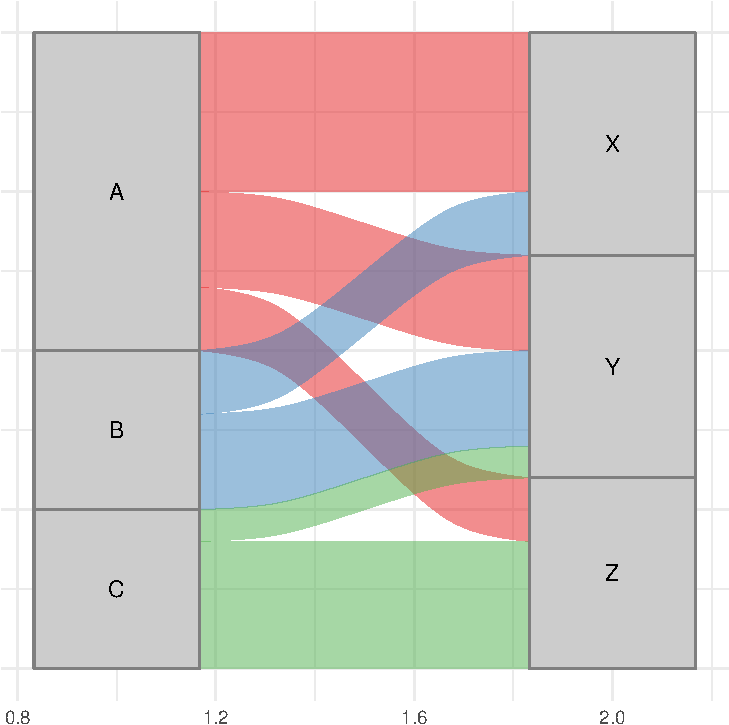
\includegraphics[keepaspectratio]{Statistik_Seminar_files/figure-beamer/unnamed-chunk-9-1.pdf}}
\end{column}
\end{columns}
\end{frame}

\begin{frame}{Horizontal Bar Chart}
\protect\phantomsection\label{horizontal-bar-chart}
\begin{columns}[T]
\begin{column}{0.6\linewidth}
\begin{itemize}
\tightlist
\item
  Vergleicht Werte über Kategorien hinweg
\item
  Horizontale Anordnung für bessere Lesbarkeit
\item
  Ideal für lange Namen oder viele Kategorien
\item
  Perfekt für Rankings und Wertvergleiche
\item
  Einfach und übersichtlich
\end{itemize}
\end{column}

\begin{column}{0.4\linewidth}
\pandocbounded{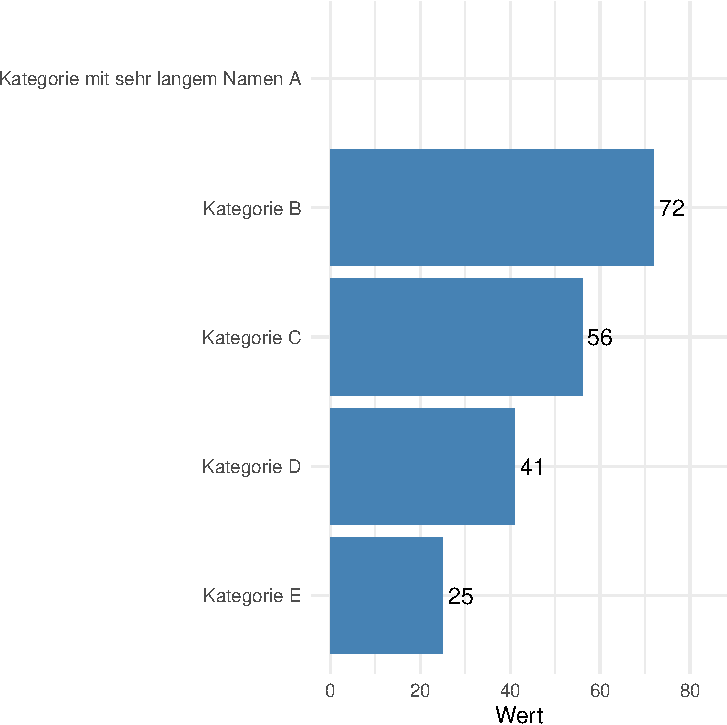
\includegraphics[keepaspectratio]{Statistik_Seminar_files/figure-beamer/unnamed-chunk-10-1.pdf}}
\end{column}
\end{columns}
\end{frame}

\begin{frame}{Column Chart}
\protect\phantomsection\label{column-chart}
\begin{columns}[T]
\begin{column}{0.6\linewidth}
\begin{itemize}
\tightlist
\item
  Vergleicht Werte mit vertikalen Balken
\item
  Ideal für Ranking und Leistungsvergleiche
\item
  Funktioniert gut mit wenigen, klaren Kategorien
\item
  Kurze, lesbare Beschriftungen bevorzugen
\item
  Konsistente Nullbasislinie für faire Vergleiche
\end{itemize}
\end{column}

\begin{column}{0.4\linewidth}
\pandocbounded{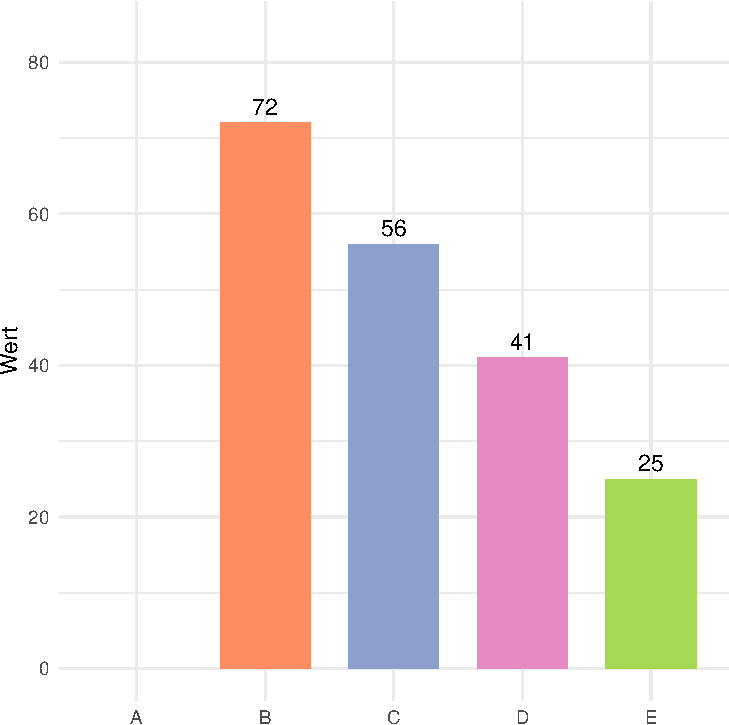
\includegraphics[keepaspectratio]{Statistik_Seminar_files/figure-beamer/unnamed-chunk-11-1.pdf}}
\end{column}
\end{columns}
\end{frame}

\begin{frame}{Vergleich: Horizontal vs.~Vertical Bar Charts}
\protect\phantomsection\label{vergleich-horizontal-vs.-vertical-bar-charts}
{\def\LTcaptype{none} % do not increment counter
\begin{longtable}[]{@{}
  >{\raggedright\arraybackslash}p{(\linewidth - 4\tabcolsep) * \real{0.3333}}
  >{\raggedright\arraybackslash}p{(\linewidth - 4\tabcolsep) * \real{0.3333}}
  >{\raggedright\arraybackslash}p{(\linewidth - 4\tabcolsep) * \real{0.3333}}@{}}
\toprule\noalign{}
\begin{minipage}[b]{\linewidth}\raggedright
Feature
\end{minipage} & \begin{minipage}[b]{\linewidth}\raggedright
Horizontal
\end{minipage} & \begin{minipage}[b]{\linewidth}\raggedright
Vertical
\end{minipage} \\
\midrule\noalign{}
\endhead
Best for & Long category labels, many items & Time-based or logical
progression \\
Readability & Easier when labels are long & Requires rotation for long
labels \\
Use case & Rankings, survey responses & Trends over time, grouped
comparisons \\
Scan direction & Left to right & Bottom to top \\
Visual space & Efficient for many categories & Better for fewer,
high-impact bars \\
\bottomrule\noalign{}
\end{longtable}
}
\end{frame}

\begin{frame}{Diverging Bars}
\protect\phantomsection\label{diverging-bars}
\begin{columns}[T]
\begin{column}{0.6\linewidth}
\begin{itemize}
\tightlist
\item
  Zeigt Abweichungen in zwei Richtungen
\item
  Links/rechts von zentraler Basislinie
\item
  Ideal für Kontraste (positiv/negativ)
\item
  Zeigt Gleichgewicht vs.~Ungleichgewicht
\item
  Gut für normalisierte Werte oder Z-Scores
\end{itemize}
\end{column}

\begin{column}{0.4\linewidth}
\pandocbounded{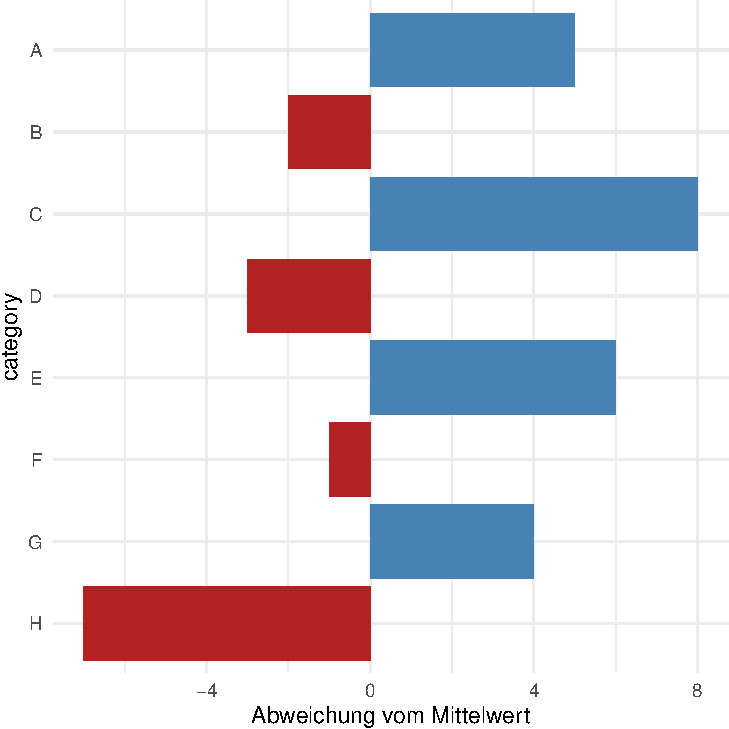
\includegraphics[keepaspectratio]{Statistik_Seminar_files/figure-beamer/unnamed-chunk-12-1.pdf}}
\end{column}
\end{columns}
\end{frame}

\begin{frame}{Diverging Lollipop Chart}
\protect\phantomsection\label{diverging-lollipop-chart}
\begin{columns}[T]
\begin{column}{0.6\linewidth}
\begin{itemize}
\tightlist
\item
  Elegantere Alternative zu Diverging Bars
\item
  Nutzt Punkte statt Balken (weniger Tinte)
\item
  Zeigt Richtung und Magnitude effektiv
\item
  Ideal wenn genaue Werte sekundär sind
\item
  Besonders gut für Präsentationen
\end{itemize}
\end{column}

\begin{column}{0.4\linewidth}
\pandocbounded{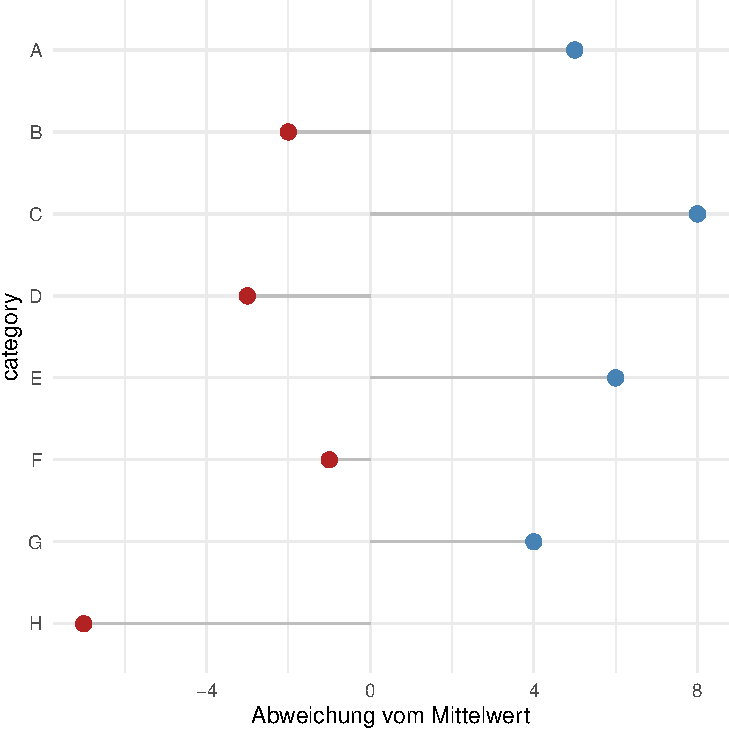
\includegraphics[keepaspectratio]{Statistik_Seminar_files/figure-beamer/unnamed-chunk-13-1.pdf}}
\end{column}
\end{columns}
\end{frame}

\begin{frame}{Histogram}
\protect\phantomsection\label{histogram}
\begin{columns}[T]
\begin{column}{0.6\linewidth}
\begin{itemize}
\tightlist
\item
  Zeigt Verteilung numerischer Daten in Bins
\item
  Balken zeigen Häufigkeiten in Wertebereichen
\item
  Erkennt Schiefe, Streuung und Ausreißer
\item
  Zeigt Modi und Clustering in Daten
\item
  Berührende Balken betonen Kontinuität
\end{itemize}
\end{column}

\begin{column}{0.4\linewidth}
\pandocbounded{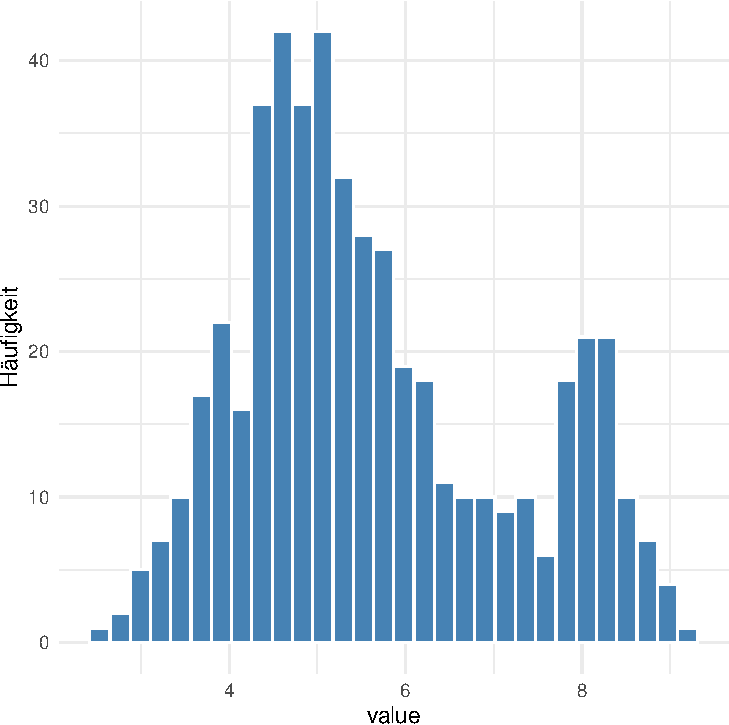
\includegraphics[keepaspectratio]{Statistik_Seminar_files/figure-beamer/unnamed-chunk-14-1.pdf}}
\end{column}
\end{columns}
\end{frame}

\begin{frame}{Boxplots}
\protect\phantomsection\label{boxplots}
\begin{columns}[T]
\begin{column}{0.6\linewidth}
\begin{itemize}
\tightlist
\item
  Zeigt Minimum, Quartile und Median
\item
  Kompakte Darstellung von Verteilungen
\item
  Hebt Streuung und Ausreißer hervor
\item
  Ideal zum Kategorienvergleich
\item
  Kann für Laien schwer verständlich sein
\end{itemize}
\end{column}

\begin{column}{0.4\linewidth}
\pandocbounded{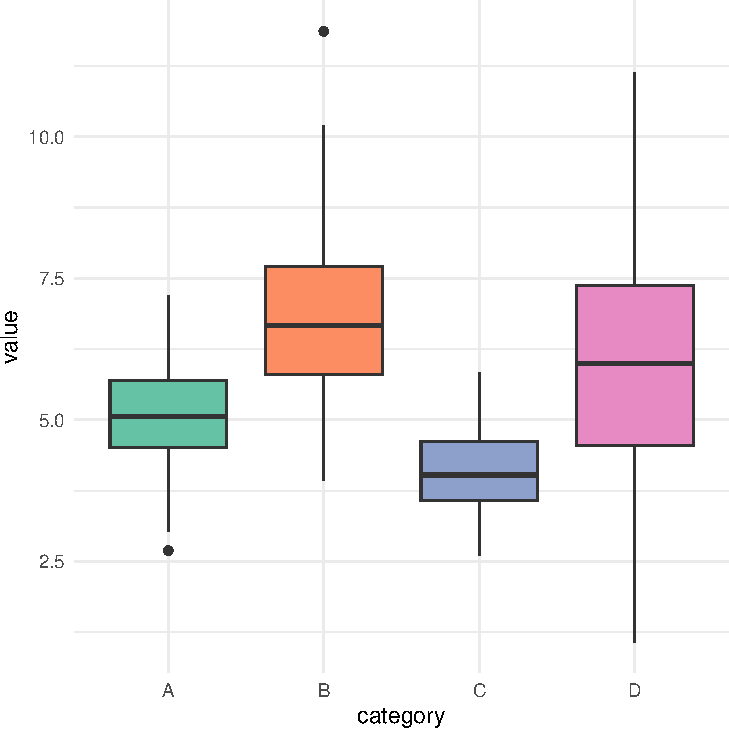
\includegraphics[keepaspectratio]{Statistik_Seminar_files/figure-beamer/unnamed-chunk-15-1.pdf}}
\end{column}
\end{columns}
\end{frame}

\begin{frame}{Boxplot mit unseren Verspätungsdaten}
\protect\phantomsection\label{boxplot-mit-unseren-verspuxe4tungsdaten}
\pandocbounded{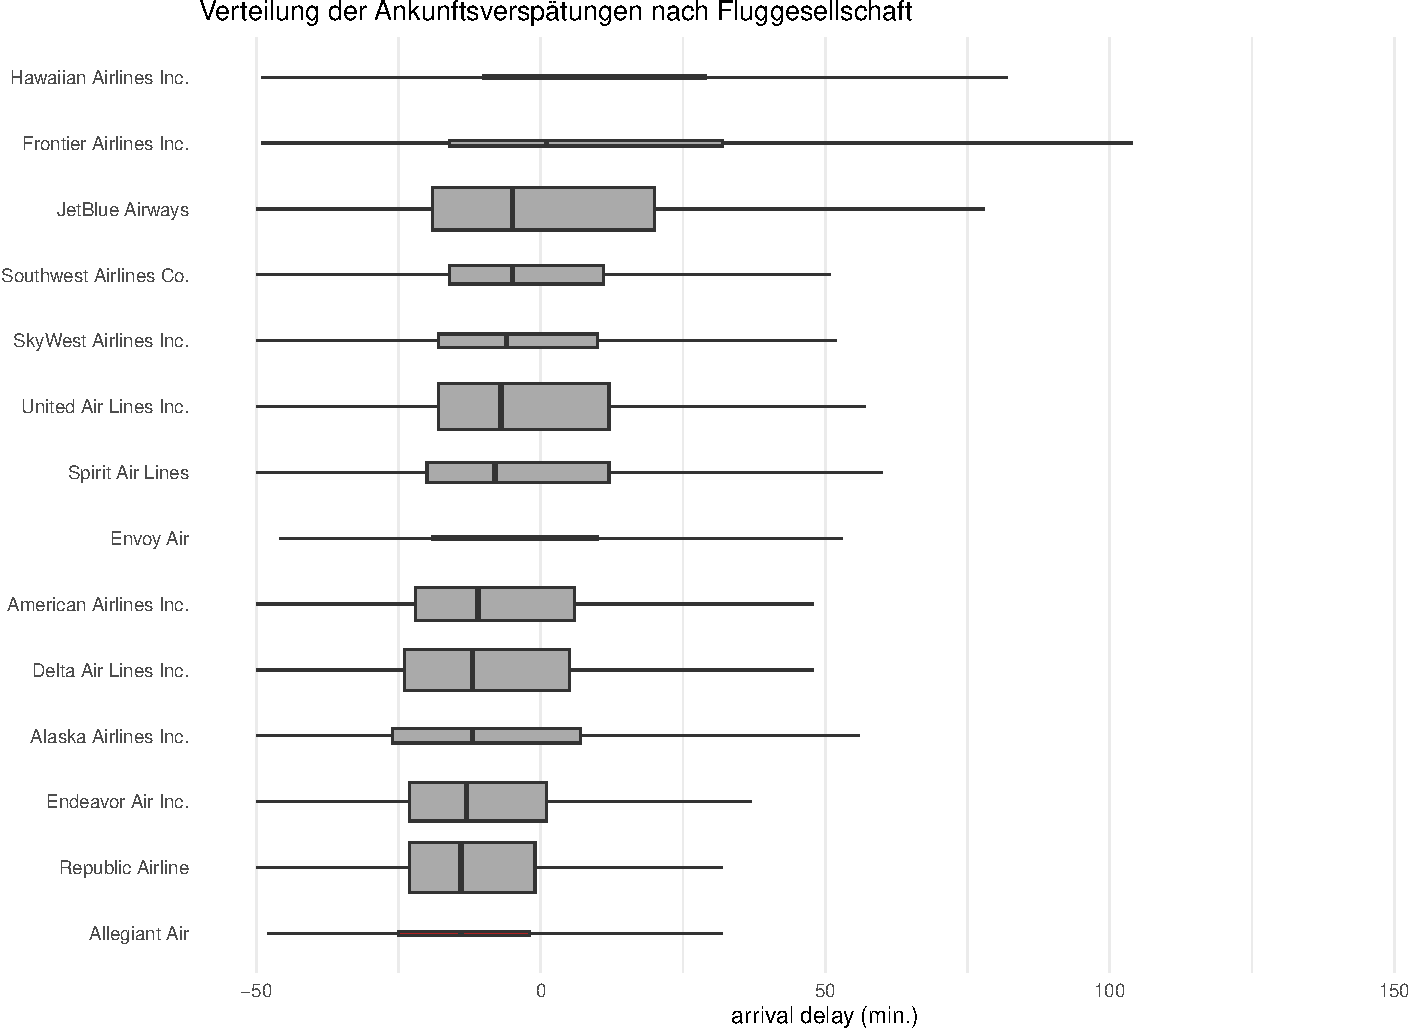
\includegraphics[keepaspectratio]{Statistik_Seminar_files/figure-beamer/unnamed-chunk-16-1.pdf}}
\end{frame}

\begin{frame}{Boxplots mit Violin Plot}
\protect\phantomsection\label{boxplots-mit-violin-plot}
\begin{columns}[T]
\begin{column}{0.6\linewidth}
\begin{itemize}
\tightlist
\item
  Kombiniert Boxplot mit Dichteverteilung
\item
  Zeigt Form, Streuung und zentrale Tendenz
\item
  Ideal für Gruppenvergleiche
\item
  Verdeutlicht Schiefe und Multimodalität
\item
  Informationsreichere Alternative zum Boxplot
\end{itemize}
\end{column}

\begin{column}{0.4\linewidth}
\pandocbounded{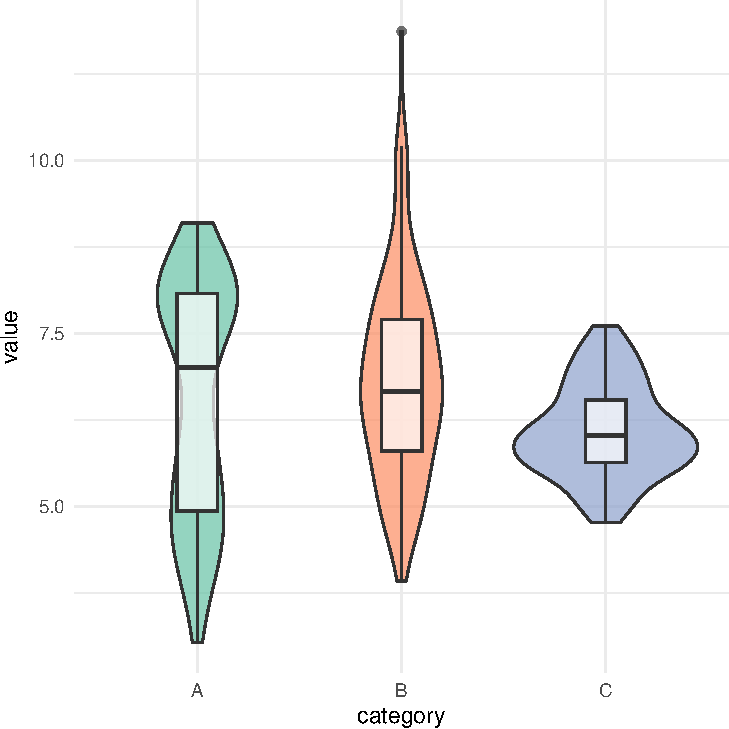
\includegraphics[keepaspectratio]{Statistik_Seminar_files/figure-beamer/unnamed-chunk-17-1.pdf}}
\end{column}
\end{columns}
\end{frame}

\begin{frame}{Choropleth Map}
\protect\phantomsection\label{choropleth-map}
\begin{columns}[T]
\begin{column}{0.6\linewidth}
\begin{itemize}
\tightlist
\item
  Färbt Regionen basierend auf Datenwerten
\item
  Zeigt räumliche Muster und Unterschiede
\item
  Gut für Verhältnisse und Prozentsätze
\item
  Nutze normalisierte Daten (pro Kopf, \%)
\item
  Vorsicht bei großen Flächenunterschieden
\end{itemize}
\end{column}

\begin{column}{0.4\linewidth}
\pandocbounded{\includegraphics[keepaspectratio]{images/map.png}}
\end{column}
\end{columns}
\end{frame}

\begin{frame}{Stacked Area Chart}
\protect\phantomsection\label{stacked-area-chart}
\begin{columns}[T]
\begin{column}{0.6\linewidth}
\begin{itemize}
\tightlist
\item
  Zeigt Kategorienbeiträge im Zeitverlauf
\item
  Gestapelte Schichten zeigen Gesamtsumme
\item
  Gut für Wachstum und Anteile
\item
  Funktioniert am besten mit wenigen Kategorien
\item
  Einzelsegmentvergleich schwierig
\end{itemize}
\end{column}

\begin{column}{0.4\linewidth}
\pandocbounded{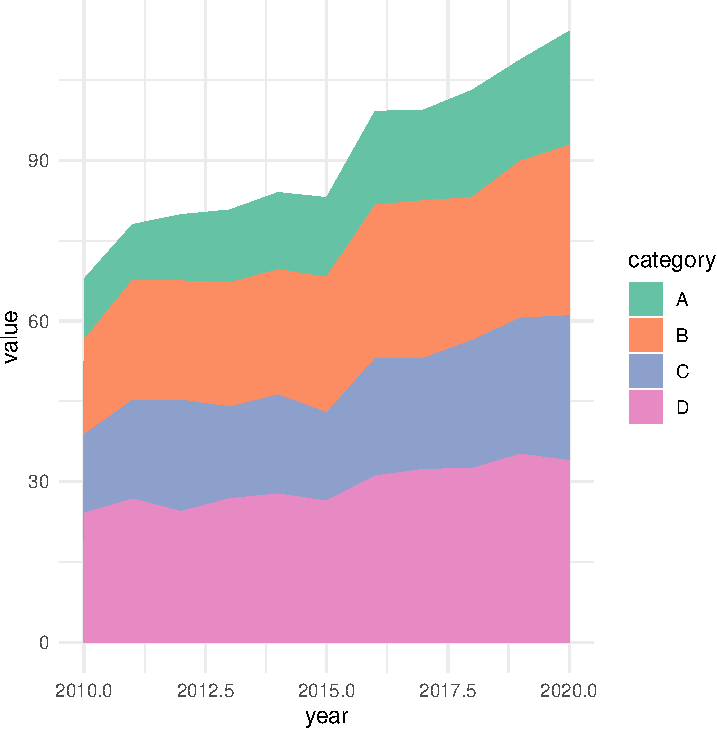
\includegraphics[keepaspectratio]{Statistik_Seminar_files/figure-beamer/unnamed-chunk-18-1.pdf}}
\end{column}
\end{columns}
\end{frame}

\begin{frame}{Stacked 100\% Area Chart}
\protect\phantomsection\label{stacked-100-area-chart}
\begin{columns}[T]
\begin{column}{0.6\linewidth}
\begin{itemize}
\tightlist
\item
  Zeigt relative Anteile, nicht absolute Werte
\item
  Verfolgt Änderungen von Kategorienanteilen
\item
  Summe immer 100\% für leichte Vergleichbarkeit
\item
  Fokus auf Zusammensetzung, nicht Wachstum
\item
  Absolute Trends gehen verloren
\end{itemize}
\end{column}

\begin{column}{0.4\linewidth}
\pandocbounded{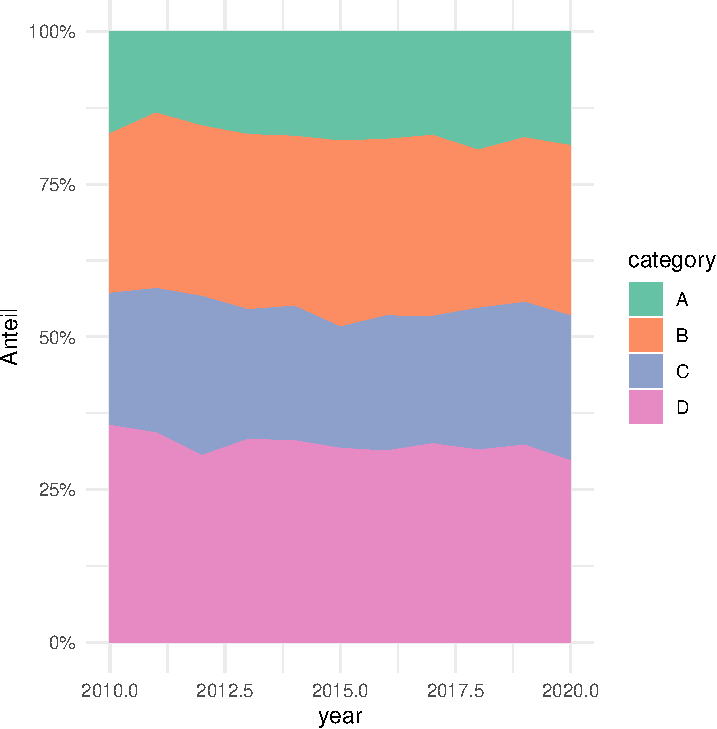
\includegraphics[keepaspectratio]{Statistik_Seminar_files/figure-beamer/unnamed-chunk-19-1.pdf}}
\end{column}
\end{columns}
\end{frame}

\begin{frame}{Stacked 100\% Area Chart Beispiel}
\protect\phantomsection\label{stacked-100-area-chart-beispiel}
\pandocbounded{\includegraphics[keepaspectratio]{images/earth_overshoot_day.png}}
\end{frame}

\begin{frame}{Waterfall Diagram}
\protect\phantomsection\label{waterfall-diagram}
\begin{columns}[T]
\begin{column}{0.6\linewidth}
\begin{itemize}
\tightlist
\item
  Zeigt Beiträge zu einer Gesamtsumme
\item
  Visualisiert Zu- und Abnahmen über Kategorien
\item
  Hebt schrittweise Veränderungen hervor
\item
  Ideal für Gewinn- oder Budgetanalysen
\item
  Zeigt Faktoren für das Endergebnis
\end{itemize}
\end{column}

\begin{column}{0.4\linewidth}
\pandocbounded{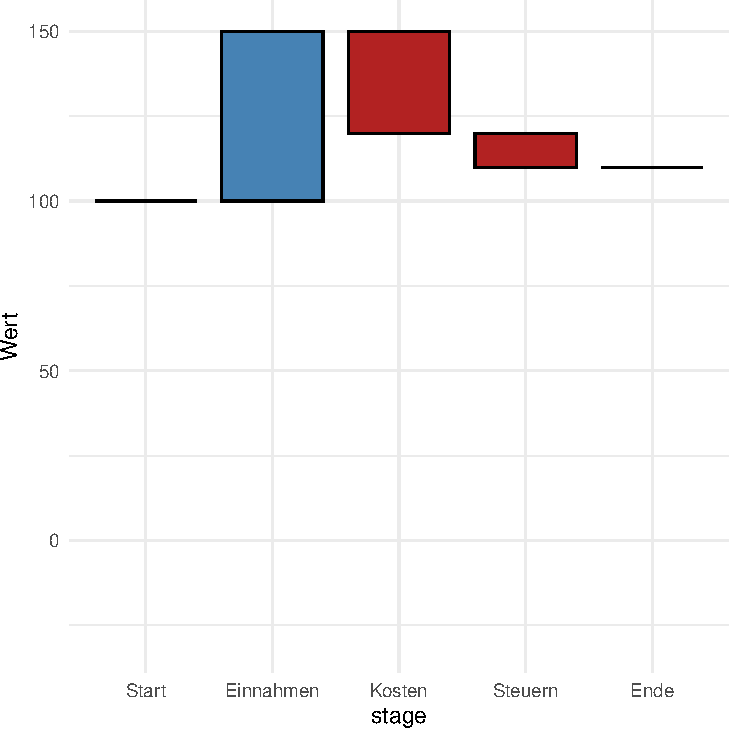
\includegraphics[keepaspectratio]{Statistik_Seminar_files/figure-beamer/unnamed-chunk-20-1.pdf}}
\end{column}
\end{columns}
\end{frame}

\begin{frame}{Heatmap}
\protect\phantomsection\label{heatmap}
\begin{columns}[T]
\begin{column}{0.6\linewidth}
\begin{itemize}
\tightlist
\item
  Nutzt Farbintensität für Matrixwerte
\item
  Zeigt Muster, Cluster und Anomalien
\item
  Gut für Korrelationen und Zeitreihen
\item
  Einfach zu überblicken, weniger präzise
\item
  Farbskala entscheidend für Interpretation
\end{itemize}
\end{column}

\begin{column}{0.4\linewidth}
\pandocbounded{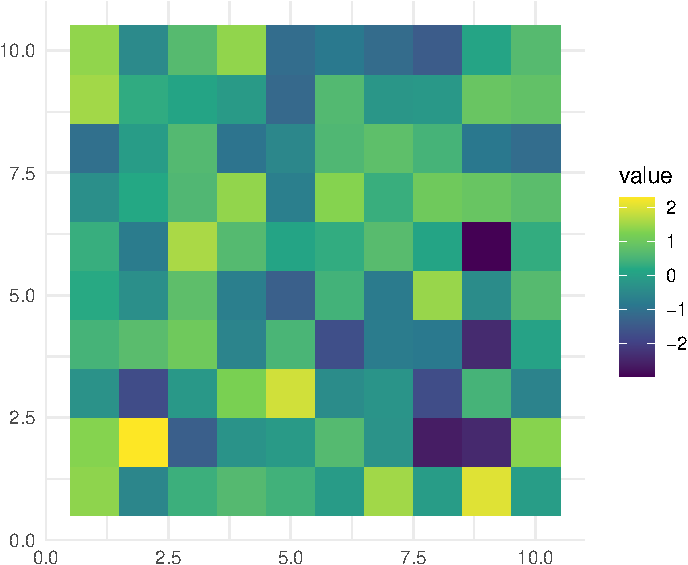
\includegraphics[keepaspectratio]{Statistik_Seminar_files/figure-beamer/unnamed-chunk-21-1.pdf}}
\end{column}
\end{columns}
\end{frame}

\begin{frame}{Treemap}
\protect\phantomsection\label{treemap}
\begin{columns}[T]
\begin{column}{0.6\linewidth}
\begin{itemize}
\tightlist
\item
  Zeigt Teil-Ganzes-Beziehungen mit Rechtecken
\item
  Größe entspricht dem Wert (Umsatz, Anzahl)
\item
  Visualisiert Hierarchien und Gruppierungen
\item
  Gut für Proportionsvergleiche
\item
  Vorsicht bei zu vielen kleinen Elementen
\end{itemize}
\end{column}

\begin{column}{0.4\linewidth}
\pandocbounded{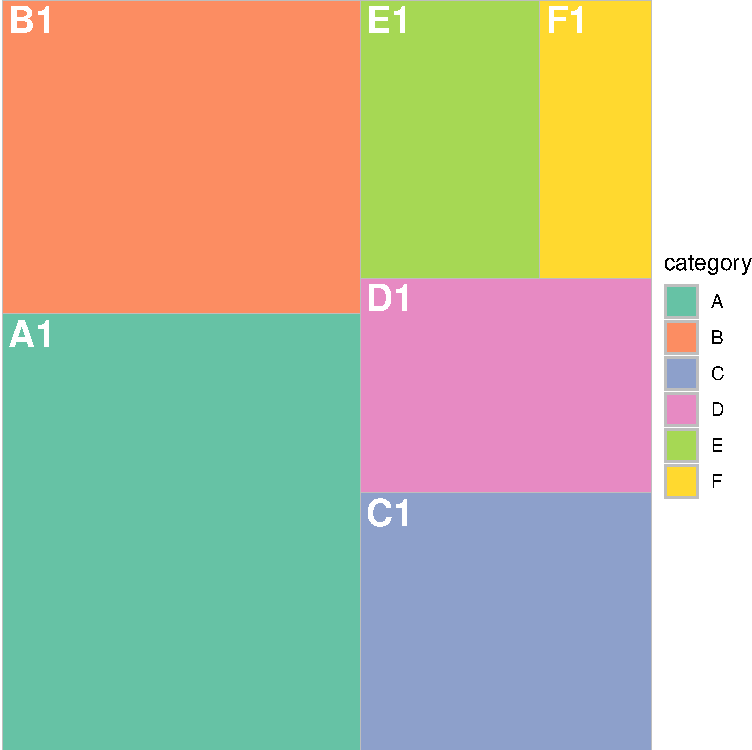
\includegraphics[keepaspectratio]{Statistik_Seminar_files/figure-beamer/unnamed-chunk-22-1.pdf}}
\end{column}
\end{columns}
\end{frame}

\begin{frame}{Treemap}
\protect\phantomsection\label{treemap-1}
\pandocbounded{\includegraphics[keepaspectratio]{images/treemap.png}}
\end{frame}

\begin{frame}{Nein, Sie verwenden bitte keine Pie Charts!}
\protect\phantomsection\label{nein-sie-verwenden-bitte-keine-pie-charts}
\pandocbounded{\includegraphics[keepaspectratio]{images/pie-chart.png}}
\end{frame}

\begin{frame}[fragile]{Datenvisualisierung mit ggplot2}
\protect\phantomsection\label{datenvisualisierung-mit-ggplot2}
\begin{itemize}
\tightlist
\item
  Base Plot vs.~ggplot2
\item
  Grammar of Graphics
\item
  \texttt{geom\_point()}, \texttt{geom\_histogram()},
  \texttt{geom\_boxplot()}
\item
  Ästhetiken: Farbe, Form, Gruppierung
\end{itemize}
\end{frame}

\section{Sitzung 6: Wahrscheinlichkeiten \&
Verteilungen}\label{sitzung-6-wahrscheinlichkeiten-verteilungen}

\begin{frame}{Lernziele dieser Sitzung}
\protect\phantomsection\label{lernziele-dieser-sitzung-4}
\begin{itemize}
\tightlist
\item
  Grundbegriffe der Wahrscheinlichkeitstheorie erklären
\item
  Diskrete und stetige Verteilungen unterscheiden
\item
  Die Normalverteilung und ihre Eigenschaften kennen
\item
  Den Zusammenhang zwischen Verteilungen und Inferenz verstehen
\end{itemize}
\end{frame}

\begin{frame}{Organisatorisches}
\protect\phantomsection\label{organisatorisches}
\begin{itemize}
\tightlist
\item
  Die Veranstaltung findet nächste Woche statt!
\item
  Zu viel los zum Semesterende? Sie können früher abgeben!
\item
  Bitte bitte bitte beachten Sie die zur Verfügung gestellten
  Materialien!
\item
  Nachtrag Stacked Area Charts
\end{itemize}
\end{frame}

\begin{frame}{Ihre Aufgabe heute}
\protect\phantomsection\label{ihre-aufgabe-heute}
\begin{enumerate}
\tightlist
\item
  Notebook ist erstellt (mit der Vorlage)
\item
  Ihre Daten sind importiert
\item
  Forschungsfragen sind ausformuliert im Notebook
\item
  \textbf{Erst dann} besprechen wir im 1:1 Ihr weiteres Vorgehen, über
  dass Sie sich \textbf{vorher} Gedanken gemacht haben
\item
  Nur wenn Sie gar nicht weiterkommen (und wirklich alle Materialien
  gesichtet haben), kommen Sie ohne diese Schritte zum 1:1
\end{enumerate}
\end{frame}

\begin{frame}{Von der Beschreibung zur Vorhersage}
\protect\phantomsection\label{von-der-beschreibung-zur-vorhersage}
\begin{itemize}
\tightlist
\item
  \textbf{Bisherige Sitzungen}: Daten beschreiben, manipulieren,
  visualisieren
\item
  \textbf{Neuer Schritt}: Von Beschreibung zu Vorhersage und
  Schlussfolgerung
\item
  \textbf{Schlüsselfrage}: Wie können wir mit Unsicherheit umgehen?
\item
  \textbf{Antwort}: Wahrscheinlichkeitstheorie als mathematisches
  Fundament
\end{itemize}
\end{frame}

\begin{frame}{Warum Wahrscheinlichkeiten für die angewandte Forschung?}
\protect\phantomsection\label{warum-wahrscheinlichkeiten-fuxfcr-die-angewandte-forschung}
\begin{itemize}
\item
  \textbf{Stichprobenlogik}\\
  → Wie kann auf eine Grundgesamtheit geschlossen werden, obwohl nur ein
  Teil beobachtet wurde?
\item
  \textbf{Unsicherheit quantifizieren}\\
  → Wie kann die Unsicherheit in empirischen Aussagen formal greifbar
  gemacht werden?
\item
  \textbf{Zufallsvariabilität verstehen}\\
  → Wie unterscheiden sich echte Effekte von zufälligen Schwankungen?
\end{itemize}
\end{frame}

\begin{frame}{Warum Wahrscheinlichkeiten für die angewandte Forschung?
Teil 2}
\protect\phantomsection\label{warum-wahrscheinlichkeiten-fuxfcr-die-angewandte-forschung-teil-2}
\begin{itemize}
\item
  \textbf{Grundlage für Inferenz}\\
  → Wahrscheinlichkeiten bilden das Fundament für Hypothesentests und
  Konfidenzintervalle.
\item
  \textbf{Bewertung von Evidenz}\\
  → Wie plausibel ist eine Theorie angesichts der beobachteten Daten?
\end{itemize}
\end{frame}

\begin{frame}{Praktische Anwendungsbeispiele}
\protect\phantomsection\label{praktische-anwendungsbeispiele}
\begin{itemize}
\tightlist
\item
  \textbf{Medizin}: Ist ein Medikament wirksam oder nur Zufall?
\item
  \textbf{Wirtschaft}: Wie wahrscheinlich ist ein Zahlungsausfall?
\item
  \textbf{Produktentwicklung}: Wie viele Nutzer werden Feature X
  verwenden?
\item
  \textbf{Marketing}: Welcher von zwei Werbetexten führt zu mehr
  Conversions?
\item
  \textbf{Qualitätssicherung}: Liegt der Produktionsprozess in
  kontrollierten Grenzen?
\end{itemize}
\end{frame}

\begin{frame}{Einführung in Wahrscheinlichkeiten}
\protect\phantomsection\label{einfuxfchrung-in-wahrscheinlichkeiten}
\begin{block}{Was ist Zufall?}
\protect\phantomsection\label{was-ist-zufall}
\end{block}
\end{frame}

\begin{frame}{Einführung in Wahrscheinlichkeiten}
\protect\phantomsection\label{einfuxfchrung-in-wahrscheinlichkeiten-1}
\begin{block}{Was ist Zufall?}
\protect\phantomsection\label{was-ist-zufall-1}
\begin{itemize}
\item
  In der Statistik beschreibt „Zufall`` das Eintreten von Ereignissen,
  deren Ergebnis nicht mit Sicherheit vorhersehbar ist, obwohl alle
  möglichen Ergebnisse bekannt sind.
\item
  Der Zufall steht nicht für Chaos, sondern für Unsicherheit bei
  einzelnen Beobachtungen. Bei vielen Wiederholungen entstehen jedoch
  erkennbare Muster (z.\,B. 50\,\% Kopf bei Münzwürfen über viele
  Versuche).
\end{itemize}
\end{block}
\end{frame}

\begin{frame}{Laplace-Wahrscheinlichkeit}
\protect\phantomsection\label{laplace-wahrscheinlichkeit}
Wenn alle Ergebnisse gleich wahrscheinlich sind, kann man die
Wahrscheinlichkeit eines Ereignisses berechnen als:

\[P(Ereignis) = \frac{\text{Anzahl günstiger Fälle}}{\text{Anzahl möglicher Fälle}}\]

\textbf{Beispiel:} Beim Würfeln ist die Wahrscheinlichkeit, eine 4 zu
würfeln: \[\frac{1}{6}\]
\end{frame}

\begin{frame}[fragile]{Empirische Wahrscheinlichkeit}
\protect\phantomsection\label{empirische-wahrscheinlichkeit}
Die empirische oder relative Häufigkeit basiert auf Beobachtungen:

\[P(Ereignis) \approx \frac{\text{Anzahl des Eintretens}}{\text{Anzahl der Wiederholungen}}\]

\textbf{Beispiel in R:}

\begin{Shaded}
\begin{Highlighting}[]
\FunctionTok{set.seed}\NormalTok{(}\DecValTok{1234}\NormalTok{)}
\NormalTok{würfe }\OtherTok{\textless{}{-}} \FunctionTok{sample}\NormalTok{(}\DecValTok{1}\SpecialCharTok{:}\DecValTok{6}\NormalTok{, }\DecValTok{1000}\NormalTok{, }\AttributeTok{replace =} \ConstantTok{TRUE}\NormalTok{)}
\FunctionTok{mean}\NormalTok{(würfe }\SpecialCharTok{==} \DecValTok{4}\NormalTok{)  }\CommentTok{\# Schätzung der Wahrscheinlichkeit für eine 4}
\end{Highlighting}
\end{Shaded}

\begin{verbatim}
[1] 0.149
\end{verbatim}
\end{frame}

\begin{frame}{Theoretische Wahrscheinlichkeit}
\protect\phantomsection\label{theoretische-wahrscheinlichkeit}
\begin{itemize}
\tightlist
\item
  Basierend auf einem \textbf{mathematischen Modell}, z.\,B. einer
  Verteilung
\item
  Wird \textbf{nicht beobachtet}, sondern \textbf{aus Annahmen
  berechnet}
\end{itemize}
\end{frame}

\begin{frame}{Theoretische Wahrscheinlichkeit}
\protect\phantomsection\label{theoretische-wahrscheinlichkeit-1}
\begin{itemize}
\tightlist
\item
  Beispiel: Wenn \[X \sim \text{Binomial}(n=10, p=0.3)\], dann ist:
\end{itemize}

\[ P(X=2) = \binom{10}{2} \cdot 0{,}3^2 \cdot 0{,}7^8 \approx 0{,}2668 \]

\begin{itemize}
\tightlist
\item
  Die theoretische Wahrscheinlichkeit gibt an, \textbf{wie
  wahrscheinlich ein Ergebnis laut Modell ist}
\end{itemize}

→ Sie ist zentral in der Inferenz: \textbf{Beobachtungen werden mit der
Theorie verglichen}
\end{frame}

\begin{frame}{Bedingte Wahrscheinlichkeit}
\protect\phantomsection\label{bedingte-wahrscheinlichkeit}
Die bedingte Wahrscheinlichkeit ( P(A\textbar B) ) beschreibt die
Wahrscheinlichkeit für A unter der Bedingung, dass B bereits eingetreten
ist.

\[P(A|B) = \frac{P(A \cap B)}{P(B)}\]

\textbf{Beispiel:} In einer medizinischen Studie haben 20\,\% der
Patienten eine Krankheit (B), und 80\,\% von diesen zeigen ein Symptom
(A). Dann ist:

\[P(A|B) = 0.8\]
\end{frame}

\begin{frame}{Beispiele von Wahrscheinlichkeiten}
\protect\phantomsection\label{beispiele-von-wahrscheinlichkeiten}
{\def\LTcaptype{none} % do not increment counter
\begin{longtable}[]{@{}
  >{\raggedright\arraybackslash}p{(\linewidth - 4\tabcolsep) * \real{0.3333}}
  >{\raggedright\arraybackslash}p{(\linewidth - 4\tabcolsep) * \real{0.3333}}
  >{\raggedright\arraybackslash}p{(\linewidth - 4\tabcolsep) * \real{0.3333}}@{}}
\toprule\noalign{}
\begin{minipage}[b]{\linewidth}\raggedright
Art
\end{minipage} & \begin{minipage}[b]{\linewidth}\raggedright
Grundlage
\end{minipage} & \begin{minipage}[b]{\linewidth}\raggedright
Beispiel
\end{minipage} \\
\midrule\noalign{}
\endhead
\textbf{Klassische (Laplace)} & Symmetrische Ausgangslage & P(4) bei
Würfel = 1/6 \\
\textbf{Empirische} & Beobachtete relative Häufigkeit & 234 von 1000
Mails geöffnet → P = 0,234 \\
\textbf{Theoretische} & Abgeleitet aus Verteilungsmodell & P(X = 2) aus
Binomial(n=10, p=0.3) \\
\textbf{Bedingte} & P(A\textbar B): A unter der Bedingung B & P(Fieber
\textbar{} krank) \\
\bottomrule\noalign{}
\end{longtable}
}
\end{frame}

\begin{frame}{Von einzelnen Wahrscheinlichkeiten zu Verteilungen}
\protect\phantomsection\label{von-einzelnen-wahrscheinlichkeiten-zu-verteilungen}
\begin{itemize}
\tightlist
\item
  Eine \textbf{Wahrscheinlichkeitsverteilung} beschreibt alle möglichen
  Ausgänge eines Zufallsexperiments und ihre Wahrscheinlichkeiten.
\end{itemize}
\end{frame}

\begin{frame}[fragile]{Zwei Typen:}
\protect\phantomsection\label{zwei-typen}
\begin{block}{Diskret (z.\,B. Würfelwurf)}
\protect\phantomsection\label{diskret-z.-b.-wuxfcrfelwurf}
\begin{itemize}
\tightlist
\item
  Endlich viele mögliche Ergebnisse
\item
  Jedem Ergebnis wird eine konkrete Wahrscheinlichkeit zugewiesen
\item
  Beispiel: P(Würfel = 4) = 1/6\\
  → Die \textbf{Verteilung} zeigt: Wie wahrscheinlich ist jede Zahl von
  1 bis 6?
\end{itemize}

\begin{Shaded}
\begin{Highlighting}[]
\FunctionTok{barplot}\NormalTok{(}\FunctionTok{rep}\NormalTok{(}\DecValTok{1}\SpecialCharTok{/}\DecValTok{6}\NormalTok{, }\DecValTok{6}\NormalTok{), }\AttributeTok{names.arg =} \DecValTok{1}\SpecialCharTok{:}\DecValTok{6}\NormalTok{, }\AttributeTok{col =} \StringTok{"skyblue"}\NormalTok{,}
        \AttributeTok{main =}\StringTok{"Diskrete Verteilung: Würfelergebnis"}\NormalTok{, }\AttributeTok{ylab =} \StringTok{"Wahrscheinlichkeit"}\NormalTok{)}
\end{Highlighting}
\end{Shaded}

\pandocbounded{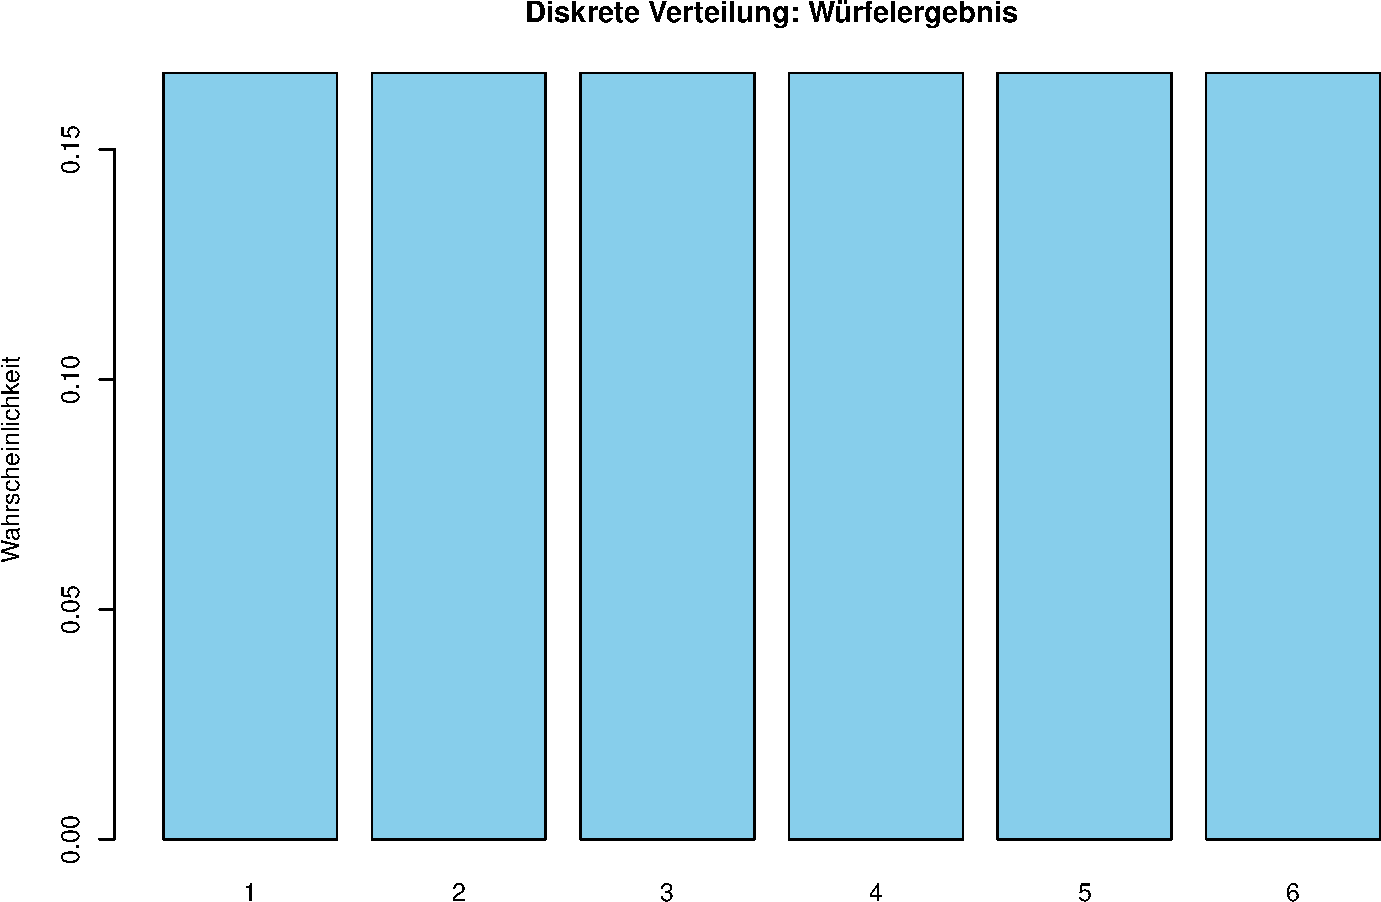
\includegraphics[keepaspectratio]{Statistik_Seminar_files/figure-beamer/unnamed-chunk-24-1.pdf}}
\end{block}

\begin{block}{Stetig (z.B. Körpergröße)}
\protect\phantomsection\label{stetig-z.b.-kuxf6rpergruxf6uxdfe}
\begin{itemize}
\tightlist
\item
  Unendlich viele mögliche Werte (z.\,B. 172,1\,cm, 172,11\,cm, \ldots)
\item
  Einzelwerte haben Wahrscheinlichkeit = 0
\item
  Stattdessen: Dichtefunktion über Intervalle
\item
  Beispiel: Wie wahrscheinlich liegt eine Körpergröße zwischen 170 und
  175\,cm?
\end{itemize}

\pandocbounded{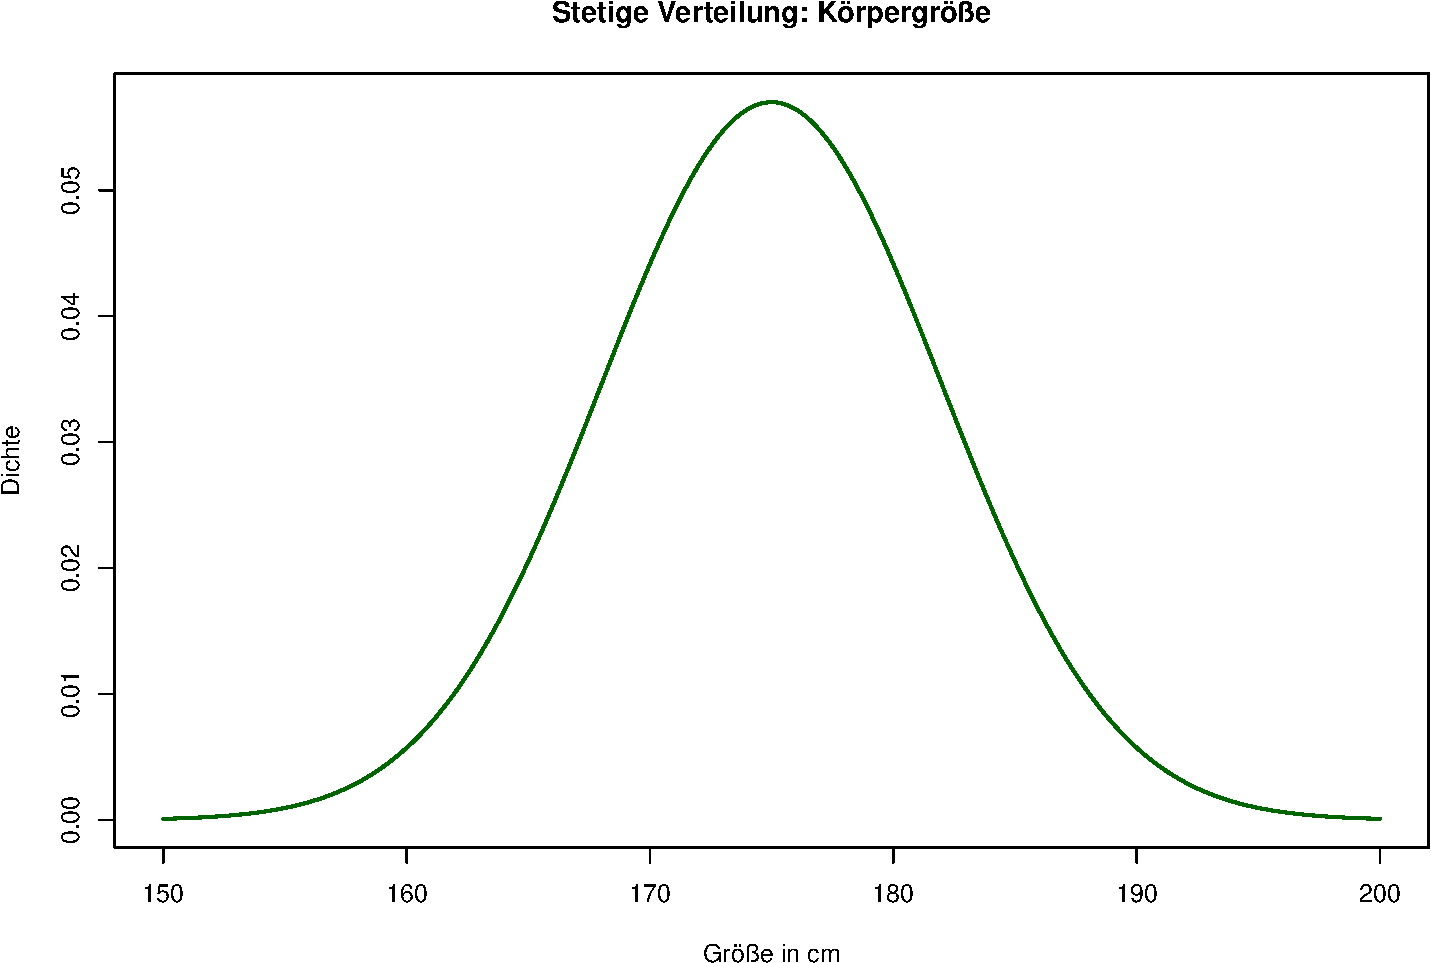
\includegraphics[keepaspectratio]{Statistik_Seminar_files/figure-beamer/unnamed-chunk-25-1.pdf}}
\end{block}
\end{frame}

\begin{frame}{Zufallsvariablen und Verteilungen}
\protect\phantomsection\label{zufallsvariablen-und-verteilungen}
\begin{itemize}
\tightlist
\item
  \textbf{Wichtige diskrete Verteilungen}:

  \begin{itemize}
  \tightlist
  \item
    Binomialverteilung (Anzahl Erfolge bei n Versuchen)
  \item
    Poisson-Verteilung (Anzahl Ereignisse in Zeitintervall)
  \end{itemize}
\item
  \textbf{Wichtige stetige Verteilungen}:

  \begin{itemize}
  \tightlist
  \item
    Gleichverteilung (konstante Wahrscheinlichkeitsdichte)
  \item
    Normalverteilung (Gaußsche Glockenkurve)
  \end{itemize}
\end{itemize}
\end{frame}

\begin{frame}{Die Normalverteilung im Detail}
\protect\phantomsection\label{die-normalverteilung-im-detail}
\begin{itemize}
\tightlist
\item
  \textbf{Eigenschaften}: Symmetrie, Mittelwert = Median = Modus
\item
  \textbf{Standardnormalverteilung}: Z-Transformation
\item
  \textbf{68-95-99,7 Regel} (Ein-, Zwei-, Dreisigma-Regel)
\item
  \textbf{Praktische Bedeutung}: Warum so viele Phänomene normalverteilt
  sind
\end{itemize}
\end{frame}

\begin{frame}{Normalverteilung in der Praxis}
\protect\phantomsection\label{normalverteilung-in-der-praxis}
\begin{itemize}
\tightlist
\item
  \textbf{Qualitätskontrolle}: Sind Abweichungen noch innerhalb der
  Spezifikation?
\item
  \textbf{Medizinische Grenzwerte}: Was ist ``normal'' bei Laborwerten?
\item
  \textbf{Notenverteilung}: Bewusster Umgang mit der Gauß'schen
  Glockenkurve
\item
  \textbf{Messfehler}: Warum kleine Abweichungen wahrscheinlicher sind
  als große
\end{itemize}
\end{frame}

\begin{frame}{Aufgabe}
\protect\phantomsection\label{aufgabe}
\begin{itemize}
\tightlist
\item
  Welche Verteilungen erwarten Sie in Ihren Forschungsfragen?
\item
  Welche Wahrscheinlichkeiten erwarten Sie?
\end{itemize}
\end{frame}

\section{Sitzung 7: Einführung in die
Inferenzstatistik}\label{sitzung-7-einfuxfchrung-in-die-inferenzstatistik}

\begin{frame}{Lernziele dieser Sitzung}
\protect\phantomsection\label{lernziele-dieser-sitzung-5}
\begin{itemize}
\tightlist
\item
  Den Zentralen Grenzwertsatz erklären und demonstrieren
\item
  Nullhypothese und Alternativhypothese formulieren
\item
  Einen t-Test in R durchführen und interpretieren
\item
  p-Wert und Konfidenzintervall korrekt kommunizieren
\item
  Fehler 1. und 2. Art sowie Effektgrößen einordnen
\end{itemize}
\end{frame}

\begin{frame}{Was ist Inferenzstatistik?}
\protect\phantomsection\label{was-ist-inferenzstatistik}
\begin{itemize}
\tightlist
\item
  Von der Stichprobe auf die Grundgesamtheit schließen
\item
  Berücksichtigt Zufallsfehler und Unsicherheit
\item
  Zentral: \textbf{Wahrscheinlichkeit}, \textbf{Stichprobenverteilung},
  \textbf{Testen von Hypothesen}
\end{itemize}
\end{frame}

\begin{frame}{Würfeln und der Zufall: Zentraler Grenzwertsatz}
\protect\phantomsection\label{wuxfcrfeln-und-der-zufall-zentraler-grenzwertsatz}
\begin{itemize}
\tightlist
\item
  Jeder Studierende würfelt 10x → 1 Mittelwert
\item
  Wiederholung über viele → Verteilung der Mittelwerte
\item
  Was ist der Erwartungswert?
\end{itemize}
\end{frame}

\begin{frame}{Würfeln und der Zufall: Zentraler Grenzwertsatz}
\protect\phantomsection\label{wuxfcrfeln-und-der-zufall-zentraler-grenzwertsatz-1}
\begin{itemize}
\tightlist
\item
  Jeder Studierende würfelt 10x → 1 Mittelwert
\item
  Wiederholung über viele → Verteilung der Mittelwerte
\item
  Erwartungswert (fairer Würfel): 3.5
\end{itemize}
\end{frame}

\begin{frame}{Würfeln und der Zufall: Zentraler Grenzwertsatz}
\protect\phantomsection\label{wuxfcrfeln-und-der-zufall-zentraler-grenzwertsatz-2}
\pandocbounded{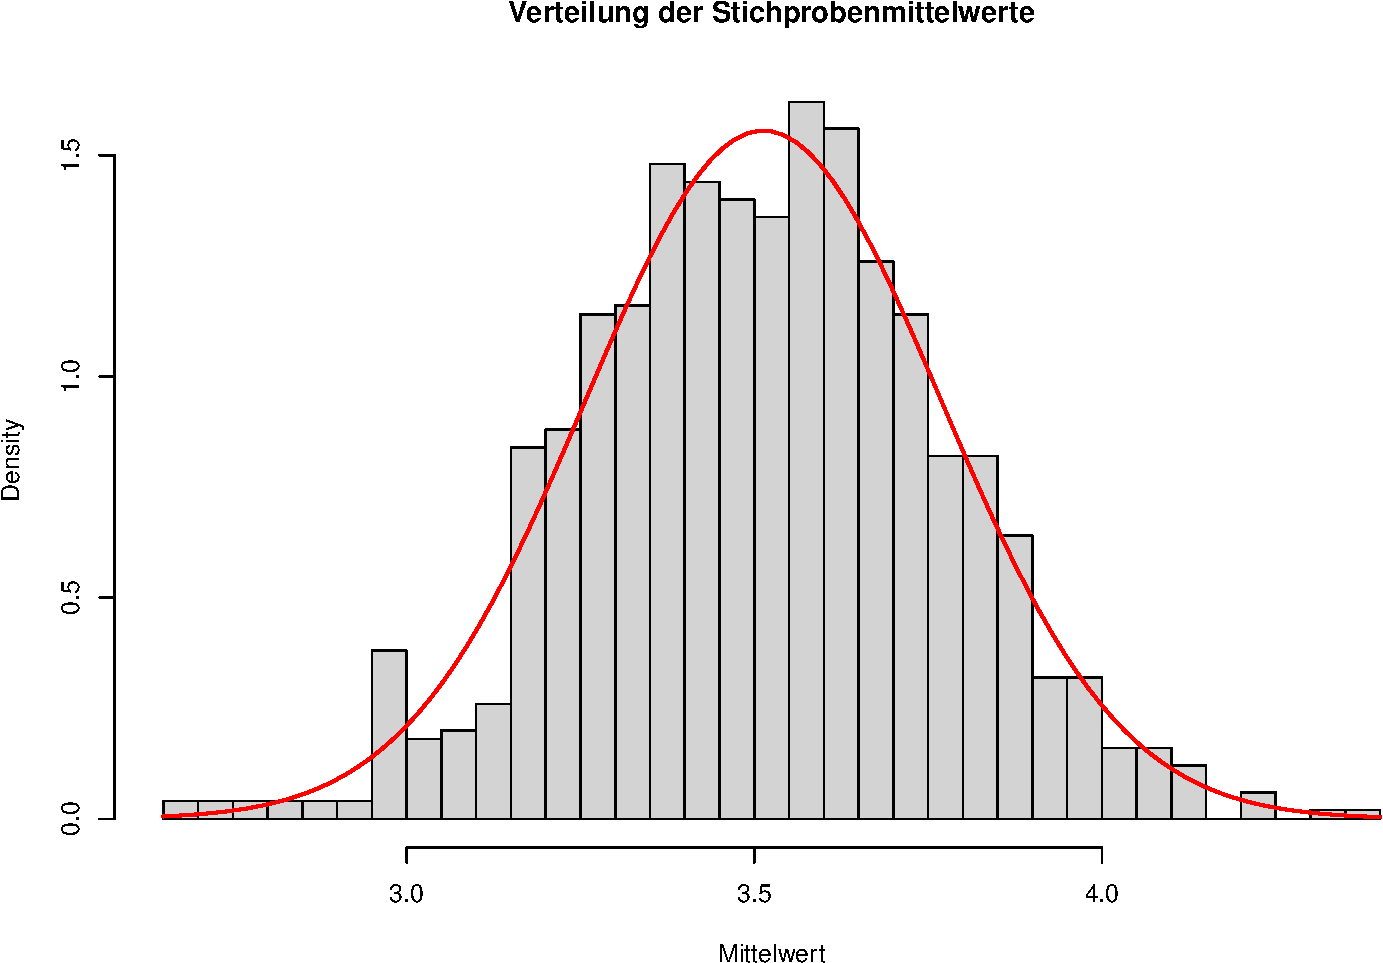
\includegraphics[keepaspectratio]{Statistik_Seminar_files/figure-beamer/unnamed-chunk-26-1.pdf}}
\end{frame}

\begin{frame}{Warum ist das wichtig?}
\protect\phantomsection\label{warum-ist-das-wichtig}
\begin{itemize}
\tightlist
\item
  Diese Verteilung erlaubt uns Aussagen über:

  \begin{itemize}
  \tightlist
  \item
    Vertrauensbereiche (Konfidenzintervalle)
  \item
    Signifikanztests (z.\,B. t-Test)
  \end{itemize}
\item
  \textbf{Beispiel}: Ist ein Würfel gezinkt?
\item
  Stichprobe: z.\,B. Mittelwert = 3.8
\item
  \textbf{Ist dieser Unterschied Zufall oder nicht?}
\end{itemize}
\end{frame}

\begin{frame}{Hypothesentesten: Grundlagen}
\protect\phantomsection\label{hypothesentesten-grundlagen}
\begin{itemize}
\tightlist
\item
  \textbf{Nullhypothese (H₀)}: Annahme keines Effekts/Unterschieds
\item
  \textbf{Alternativhypothese (H₁)}: Annahme eines Effekts/Unterschieds
\item
  \textbf{Arten von Hypothesen}:

  \begin{itemize}
  \tightlist
  \item
    Ungerichtete Hypothesen (zweiseitig): µ₁ ≠ µ₂
  \item
    Gerichtete Hypothesen (einseitig): µ₁ \textgreater{} µ₂ oder µ₁
    \textless{} µ₂
  \end{itemize}
\end{itemize}
\end{frame}

\begin{frame}{Die Logik des Hypothesentestens}
\protect\phantomsection\label{die-logik-des-hypothesentestens}
\begin{itemize}
\tightlist
\item
  \textbf{Indirekter Beweis}: Wir falsifizieren H₀ statt H₁ zu beweisen
\item
  \textbf{Analogie zum Gerichtsprozess}: ``Unschuldig bis zum Beweis der
  Schuld''
\item
  \textbf{Entscheidungsbaum}: Wann wird H₀ beibehalten oder verworfen?
\end{itemize}
\end{frame}

\begin{frame}{Signifikanzniveau und p-Wert}
\protect\phantomsection\label{signifikanzniveau-und-p-wert}
\begin{itemize}
\tightlist
\item
  \textbf{Signifikanzniveau α}: Vorab festgelegte
  Irrtumswahrscheinlichkeit (typisch: 0.05)
\item
  \textbf{p-Wert}: Wahrscheinlichkeit, die beobachteten (oder
  extremeren) Daten unter H₀ zu erhalten
\item
  \textbf{Entscheidungsregel}: Verwerfe H₀, wenn p \textless{} α
\item
  \textbf{Kritische Werte}: Alternative Darstellung der
  Entscheidungsregel
\end{itemize}
\end{frame}

\begin{frame}{Von der Stichprobenverteilung zum t-Test}
\protect\phantomsection\label{von-der-stichprobenverteilung-zum-t-test}
\begin{itemize}
\tightlist
\item
  Die \textbf{Stichprobenverteilung der Mittelwerte} zeigt: Wie stark
  Mittelwerte \textbf{zufällig schwanken}, selbst wenn H₀ stimmt
\item
  Diese Schwankung hat eine Streuung: den \textbf{Standardfehler (SE)}
\end{itemize}

\[ SE = \frac{s}{\sqrt{n}} \]

\begin{itemize}
\tightlist
\item
  Der t-Test prüft, ob der beobachtete Mittelwert \textbf{außerhalb}
  dieser erwarteten Schwankung liegt
\end{itemize}
\end{frame}

\begin{frame}[fragile]{Der Standardfehler}
\protect\phantomsection\label{der-standardfehler}
\begin{itemize}
\tightlist
\item
  \textbf{Definition}: Standardabweichung der Stichprobenmittelwerte
\item
  \textbf{Praktische Bedeutung}: Je größer die Stichprobe, desto
  präziser die Schätzung
\end{itemize}

\begin{Shaded}
\begin{Highlighting}[]
\FunctionTok{set.seed}\NormalTok{(}\DecValTok{422}\NormalTok{)}
\NormalTok{würfe }\OtherTok{\textless{}{-}} \FunctionTok{sample}\NormalTok{(}\DecValTok{1}\SpecialCharTok{:}\DecValTok{6}\NormalTok{, }\DecValTok{60}\NormalTok{, }\AttributeTok{replace =} \ConstantTok{TRUE}\NormalTok{)}
\NormalTok{se }\OtherTok{\textless{}{-}} \FunctionTok{sd}\NormalTok{(würfe) }\SpecialCharTok{/} \FunctionTok{sqrt}\NormalTok{(}\FunctionTok{length}\NormalTok{(würfe))}
\NormalTok{se}
\end{Highlighting}
\end{Shaded}

\begin{verbatim}
[1] 0.2296727
\end{verbatim}

\begin{verbatim}
[1] 3.433333
\end{verbatim}
\end{frame}

\begin{frame}[fragile]{t-Test in R (Einzelstichprobe)}
\protect\phantomsection\label{t-test-in-r-einzelstichprobe}
\begin{verbatim}
[1] 3.433333
\end{verbatim}

\begin{verbatim}

    One Sample t-test

data:  würfe
t = -0.29027, df = 59, p-value = 0.7726
alternative hypothesis: true mean is not equal to 3.5
95 percent confidence interval:
 2.973759 3.892907
sample estimates:
mean of x 
 3.433333 
\end{verbatim}
\end{frame}

\begin{frame}{Interpretation des t-Tests}
\protect\phantomsection\label{interpretation-des-t-tests}
\begin{itemize}
\tightlist
\item
  \textbf{p \textless{} 0.05} → Ablehnung der Nullhypothese (Würfel
  evtl. gezinkt)
\item
  \textbf{p ≥ 0.05} → Kein ausreichender Hinweis auf Manipulation
\end{itemize}
\end{frame}

\begin{frame}{Was ist denn nun „signifikant``?}
\protect\phantomsection\label{was-ist-denn-nun-signifikant}
\begin{itemize}
\tightlist
\item
  Ein signifikantes Ergebnis heißt nicht, dass es „wichtig`` ist
\item
  Es heißt nur: Unterschied ist \textbf{nicht gut durch Zufall
  erklärbar}
\item
  Immer im Kontext interpretieren (Effektgröße, Relevanz)
\end{itemize}
\end{frame}

\begin{frame}{Konfidenzintervalle}
\protect\phantomsection\label{konfidenzintervalle}
\begin{itemize}
\item
  \textbf{Definition}: Bereich, der mit einer bestimmten
  Wahrscheinlichkeit den wahren Parameter enthält
\item
  \textbf{Interpretation}: Was bedeutet ein 95\%-Konfidenzintervall?
\item
  \textbf{Zusammenhang mit Hypothesentests}: Enthält ein 95\%-KI den
  Wert der Nullhypothese?
\end{itemize}
\end{frame}

\begin{frame}{Experimentelles Design}
\protect\phantomsection\label{experimentelles-design}
\begin{itemize}
\tightlist
\item
  \textbf{Wichtige Konzepte}: Randomisierung, Kontrolle, Randomized
  Control Trial (RCT)
\item
  \textbf{Experimentierfehler vermeiden}:

  \begin{itemize}
  \tightlist
  \item
    Placebo-Effekt
  \item
    Hawthorne-Effekt
  \item
    Observer Bias
  \item
    Selection Bias
  \end{itemize}
\end{itemize}
\end{frame}

\begin{frame}{Ursprung der t-Verteilung: William S. Gosset}
\protect\phantomsection\label{ursprung-der-t-verteilung-william-s.-gosset}
\begin{itemize}
\tightlist
\item
  \textbf{William S. Gosset} war Chemiker und Statistiker bei der
  Guinness-Brauerei (Anfang 1900er).
\item
  Aufgabe: Qualitätskontrolle (z.\,B. Stärkegehalt von Gerste messen).
\item
  Problem: Nur \textbf{kleine Stichproben} pro Tag (z.\,B. n = 4 oder
  5).
\item
  Damalige Statistik: Basierte auf \textbf{großen Stichproben} und der
  \textbf{Normalverteilung}.
\end{itemize}
\end{frame}

\begin{frame}{Das statistische Problem}
\protect\phantomsection\label{das-statistische-problem}
\begin{itemize}
\tightlist
\item
  Ziel: Testen, ob der Mittelwert von Proben vom Sollwert abweicht.
\item
  Normalformel: {[} \frac{\bar{x} - \mu}{\sigma / \sqrt{n}} {]} →
  funktioniert nur, wenn \textbf{σ} (Standardabweichung der
  Grundgesamtheit) bekannt ist.
\item
  Bei kleinen n musste Gosset stattdessen \textbf{s}
  (Stichprobenstandardabweichung) verwenden:
  \[  \frac{\bar{x} - \mu}{s / \sqrt{n}}\]
\item
  Folge: Diese Teststatistik \textbf{folgt nicht mehr der
  Normalverteilung}.
\end{itemize}
\end{frame}

\begin{frame}{Die Lösung}
\protect\phantomsection\label{die-luxf6sung}
\begin{itemize}
\tightlist
\item
  Gosset zeigte: Die neue Verteilung hängt von der Anzahl an
  Beobachtungen ab → \textbf{Freiheitsgrade (n−1)}.
\item
  Daraus entstand eine neue Verteilung: die \textbf{t-Verteilung mit
  df}.
\item
  Diese berücksichtigt die \textbf{größere Unsicherheit bei kleinen n}
  durch dickere „Schwänze`` (heavy tails).
\end{itemize}
\end{frame}

\begin{frame}{Warum „Student``?}
\protect\phantomsection\label{warum-student}
\begin{itemize}
\tightlist
\item
  Guinness verbot es Mitarbeitern, unter eigenem Namen zu publizieren.
\item
  Gosset veröffentlichte 1908 unter dem Pseudonym \textbf{„Student``}:

  \begin{itemize}
  \tightlist
  \item
    \emph{„The Probable Error of a Mean``} (in \emph{Biometrika})
  \end{itemize}
\item
  Der t-Test wurde dadurch bekannt als \textbf{„Student's t-Test``}.
\end{itemize}
\end{frame}

\begin{frame}{Visualisierung unterschiedlicher t-Verteilungen}
\protect\phantomsection\label{visualisierung-unterschiedlicher-t-verteilungen}
\pandocbounded{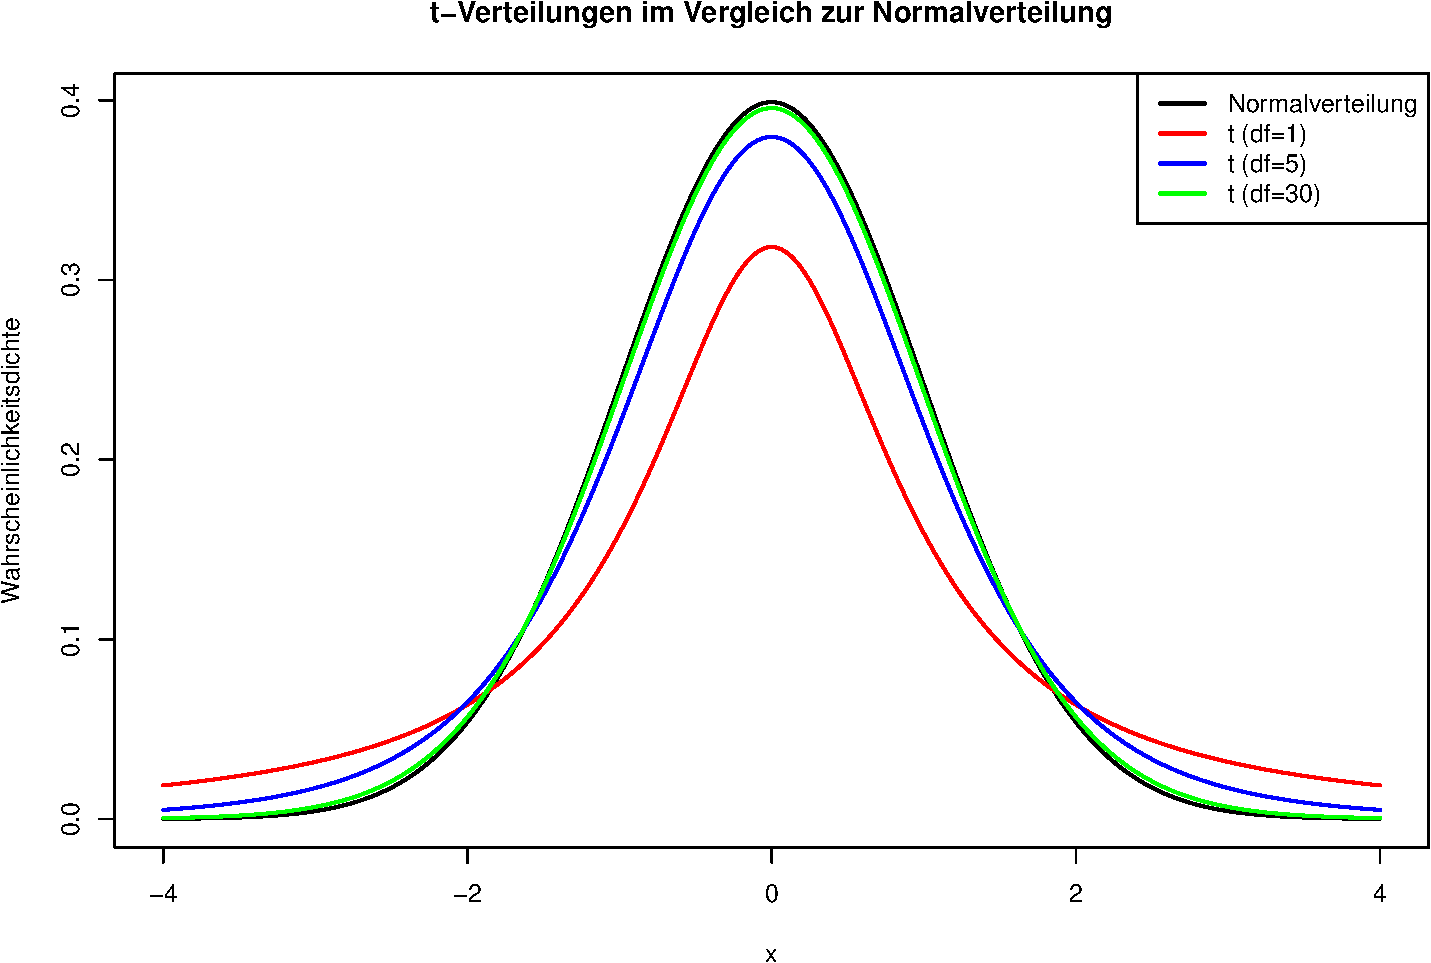
\includegraphics[keepaspectratio]{Statistik_Seminar_files/figure-beamer/unnamed-chunk-30-1.pdf}}
\end{frame}

\begin{frame}{Freiheitsgrade (Degrees of Freedom, df)}
\protect\phantomsection\label{freiheitsgrade-degrees-of-freedom-df}
\begin{itemize}
\tightlist
\item
  Anzahl der \textbf{unabhängigen Informationen}, die zur Schätzung
  einer Größe verfügbar sind.
\item
  Bei der Berechnung der \textbf{Stichprobenvarianz} geht 1
  Freiheitsgrad verloren: {[} df = n - 1 {]} (weil der Mittelwert
  bereits aus den Daten berechnet wurde)
\item
  Freiheitsgrade bestimmen die \textbf{Form der t-Verteilung}:

  \begin{itemize}
  \tightlist
  \item
    Wenige df → \textbf{dickere Randbereiche}
  \item
    Viele df → t-Verteilung nähert sich der \textbf{Normalverteilung}
  \end{itemize}
\end{itemize}
\end{frame}

\begin{frame}{Freiheitsgrade (Degrees of Freedom, df)}
\protect\phantomsection\label{freiheitsgrade-degrees-of-freedom-df-1}
\begin{itemize}
\tightlist
\item
  Freiheitsgrade sind wichtig für:

  \begin{itemize}
  \tightlist
  \item
    Auswahl des richtigen \textbf{kritischen t-Werts}
  \item
    \textbf{Vertrauensintervalle} und \textbf{p-Werte}
  \end{itemize}
\end{itemize}
\end{frame}

\begin{frame}{Arten von t-Tests}
\protect\phantomsection\label{arten-von-t-tests}
\begin{itemize}
\tightlist
\item
  \textbf{Einstichproben-t-Test}: Vergleich mit bekanntem oder
  hypothetischem Wert

  \begin{itemize}
  \tightlist
  \item
    Anwendungsbeispiel: Entspricht der mittlere Blutzuckerwert einer
    Patientengruppe dem Normalwert?
  \item
    Formel: \(t = \frac{\bar{x} - \mu_0}{s / \sqrt{n}}\)
  \end{itemize}
\end{itemize}
\end{frame}

\begin{frame}{Arten von t-Tests}
\protect\phantomsection\label{arten-von-t-tests-1}
\begin{itemize}
\tightlist
\item
  \textbf{Zweistichproben-t-Test (unabhängig)}: Vergleich zweier
  unabhängiger Gruppen

  \begin{itemize}
  \tightlist
  \item
    Anwendungsbeispiel: Unterscheiden sich die Testergebnisse zweier
    unterschiedlicher Lernmethoden?
  \item
    Formel bei gleichen Varianzen:
    \(t = \frac{\bar{x}_1 - \bar{x}_2}{s_p \sqrt{\frac{1}{n_1} + \frac{1}{n_2}}}\)
  \end{itemize}
\end{itemize}
\end{frame}

\begin{frame}{Arten von t-Tests}
\protect\phantomsection\label{arten-von-t-tests-2}
\begin{itemize}
\tightlist
\item
  \textbf{Gepaarter t-Test (abhängig)}: Vergleich verbundener Messungen

  \begin{itemize}
  \tightlist
  \item
    Anwendungsbeispiel: Vor-Nach-Vergleich einer Intervention
  \item
    Formel: \(t = \frac{\bar{d}}{s_d / \sqrt{n}}\)
  \end{itemize}
\end{itemize}
\end{frame}

\begin{frame}{Arten von t-Tests}
\protect\phantomsection\label{arten-von-t-tests-3}
\begin{itemize}
\tightlist
\item
  \textbf{Welch-Test}: Variante für ungleiche Varianzen

  \begin{itemize}
  \tightlist
  \item
    Anwendungsbeispiel: Wenn die Streuung in beiden Gruppen deutlich
    unterschiedlich ist
  \item
    Angepasste Freiheitsgrade
  \end{itemize}
\end{itemize}
\end{frame}

\begin{frame}{Voraussetzungen der t-Tests}
\protect\phantomsection\label{voraussetzungen-der-t-tests}
\begin{itemize}
\tightlist
\item
  \textbf{Normalverteilung}: Robustheit bei Verletzungen
\item
  \textbf{Varianzhomogenität}: Bedeutung und Tests (Levene-Test, F-Test)
\item
  \textbf{Unabhängigkeit der Beobachtungen}: Kritisch für die Gültigkeit
\item
  \textbf{Zentraler Grenzwertsatz als Rettungsanker}: Wann können wir
  uns darauf verlassen?
\end{itemize}
\end{frame}

\begin{frame}{Interpretation und Berichterstattung}
\protect\phantomsection\label{interpretation-und-berichterstattung}
\begin{itemize}
\tightlist
\item
  \textbf{Angabe des Konfidenzintervalls}: Zusätzliche Information zur
  Präzision
\item
  \textbf{Standardisierte Berichtsform}: APA-Style für wissenschaftliche
  Publikationen
\item
  \textbf{Beispiel}: ``Ein unabhängiger t-Test zeigte einen
  signifikanten Unterschied zwischen den Gruppen (t(28) = 2.45, p =
  0.02, d = 0.89). Die Experimentalgruppe (M = 25.3, SD = 4.2) erzielte
  höhere Werte als die Kontrollgruppe (M = 21.7, SD = 3.8).''
\end{itemize}
\end{frame}

\begin{frame}{Fehler beim Hypothesentesten}
\protect\phantomsection\label{fehler-beim-hypothesentesten}
\begin{itemize}
\tightlist
\item
  \textbf{Fehler 1. Art (α-Fehler)}: Falsch-positive Entscheidung (H₀
  fälschlicherweise verwerfen)
\item
  \textbf{Fehler 2. Art (β-Fehler)}: Falsch-negative Entscheidung (H₀
  fälschlicherweise beibehalten)
\item
  \textbf{Power (1-β)}: Wahrscheinlichkeit, einen tatsächlich
  vorhandenen Effekt zu entdecken
\item
  \textbf{Balanceakt}: Abwägung zwischen α und β
\end{itemize}
\end{frame}

\begin{frame}{Effektgröße beim t-Test: Cohen's d}
\protect\phantomsection\label{effektgruxf6uxdfe-beim-t-test-cohens-d}
\textbf{Das Problem:}

t = 3.45, p = 0.001 → ``Signifikant!''

\textbf{Aber wie groß ist der Unterschied wirklich?}

\textbf{Cohen's d Formel:}
\[d = \frac{\bar{x}_1 - \bar{x}_2}{s_{pooled}}\]
\end{frame}

\begin{frame}{Interpretation nach Cohen}
\protect\phantomsection\label{interpretation-nach-cohen}
{\def\LTcaptype{none} % do not increment counter
\begin{longtable}[]{@{}lll@{}}
\toprule\noalign{}
Cohen's d & Effektgröße & Beispiel \\
\midrule\noalign{}
\endhead
\textbf{0.2} & Klein & Männer vs.~Frauen: Körpergröße \\
\textbf{0.5} & Mittel & Therapie vs.~Kontrollgruppe \\
\textbf{0.8} & Groß & Experten vs.~Anfänger \\
\bottomrule\noalign{}
\end{longtable}
}
\end{frame}

\begin{frame}{Vier kritische Szenarien}
\protect\phantomsection\label{vier-kritische-szenarien}
{\def\LTcaptype{none} % do not increment counter
\begin{longtable}[]{@{}lll@{}}
\toprule\noalign{}
p-Wert & Cohen's d & Interpretation \\
\midrule\noalign{}
\endhead
p \textgreater{} 0.05 & d \textless{} 0.2 & ✅ Kein Effekt \\
p \textgreater{} 0.05 & d \textgreater{} 0.5 & ⚠️ Zu kleine
Stichprobe \\
p \textless{} 0.05 & d \textgreater{} 0.5 & ✅ Signifikant \&
bedeutsam \\
p \textless{} 0.05 & d \textless{} 0.2 & ❌ \textbf{``Signifikant
trivial''} \\
\bottomrule\noalign{}
\end{longtable}
}
\end{frame}

\section{Sitzung 8: Chi-Quadrat-Test für
Häufigkeiten}\label{sitzung-8-chi-quadrat-test-fuxfcr-huxe4ufigkeiten}

\begin{frame}{Lernziele dieser Sitzung}
\protect\phantomsection\label{lernziele-dieser-sitzung-6}
\begin{itemize}
\tightlist
\item
  Den Chi-Quadrat-Test für kategoriale Daten anwenden
\item
  Anpassungstest und Unabhängigkeitstest unterscheiden
\item
  Residuen und Effektstärken (Cramér's V) berechnen und interpretieren
\item
  Voraussetzungen prüfen und Alternativen kennen (Fisher's Exakter Test)
\end{itemize}
\end{frame}

\begin{frame}{Rückblick: Von t-Tests zu kategorialen Daten}
\protect\phantomsection\label{ruxfcckblick-von-t-tests-zu-kategorialen-daten}
\begin{itemize}
\tightlist
\item
  \textbf{Letzte Woche}: t-Tests für kontinuierliche Daten (Mittelwerte)
\item
  \textbf{Heute}: Tests für kategoriale Daten (Häufigkeiten)
\item
  \textbf{Verbindung}: Beide testen Hypothesen, aber mit verschiedenen
  Datentypen
\item
  \textbf{Beispiel}: Statt ``Ist der mittlere Würfelwert 3.5?'' → ``Sind
  alle Würfelseiten gleich häufig?''
\end{itemize}
\end{frame}

\begin{frame}{Würfel-Motivation: Ein praktisches Problem}
\protect\phantomsection\label{wuxfcrfel-motivation-ein-praktisches-problem}
\textbf{Situation}: Ein Freund behauptet, sein Würfel sei fair

\textbf{Daten sammeln}: 60 Würfe

\begin{itemize}
\tightlist
\item
  1er: 8 mal
\item
  2er: 12 mal
\item
  3er: 9 mal
\item
  4er: 11 mal
\item
  5er: 10 mal
\item
  6er: 10 mal
\end{itemize}
\end{frame}

\begin{frame}{Würfel-Motivation: Ein praktisches Problem}
\protect\phantomsection\label{wuxfcrfel-motivation-ein-praktisches-problem-1}
\textbf{Fragen}:

\begin{itemize}
\item
  Ist dieser Würfel fair?
\item
  Wie können wir das statistisch testen?
\item
  Was erwarten wir bei einem fairen Würfel?
\end{itemize}

\textbf{Bei fairem Würfel}: Jede Zahl sollte etwa 10 mal fallen (60 ÷ 6
= 10)
\end{frame}

\begin{frame}[fragile]{Einführung in kategoriale Datenanalyse}
\protect\phantomsection\label{einfuxfchrung-in-kategoriale-datenanalyse}
\begin{itemize}
\tightlist
\item
  \textbf{Charakteristika kategorialer Daten}:

  \begin{itemize}
  \tightlist
  \item
    Nominal (Geschlecht, Farben, Würfelzahlen)
  \item
    Ordinal (Schulnoten, Zufriedenheitsskalen)
  \end{itemize}
\item
  \textbf{Häufigkeitstabellen}: Absolute und relative Häufigkeiten
\item
  \textbf{Kontingenztabellen}: Darstellung von Zusammenhängen zwischen
  kategorialen Variablen
\end{itemize}

\begin{verbatim}
würfel_daten
 1  2  3  4  5  6 
 8 12  9 11 10 10 
\end{verbatim}
\end{frame}

\begin{frame}{Der Chi-Quadrat-Test: Grundprinzip}
\protect\phantomsection\label{der-chi-quadrat-test-grundprinzip}
\begin{itemize}
\tightlist
\item
  \textbf{Kernidee}: Vergleich beobachteter und erwarteter Häufigkeiten
\item
  \textbf{Formel}: \(\chi^2 = \sum \frac{(O - E)^2}{E}\)

  \begin{itemize}
  \tightlist
  \item
    O: beobachtete Häufigkeit (observed)
  \item
    E: erwartete Häufigkeit (expected)
  \end{itemize}
\item
  \textbf{Logik}: Große Abweichungen → große χ²-Werte → Hinweis auf
  Unterschied
\end{itemize}
\end{frame}

\begin{frame}
\end{frame}

\begin{frame}{Visualisierung: Beobachtet vs Erwartet}
\protect\phantomsection\label{visualisierung-beobachtet-vs-erwartet}
\pandocbounded{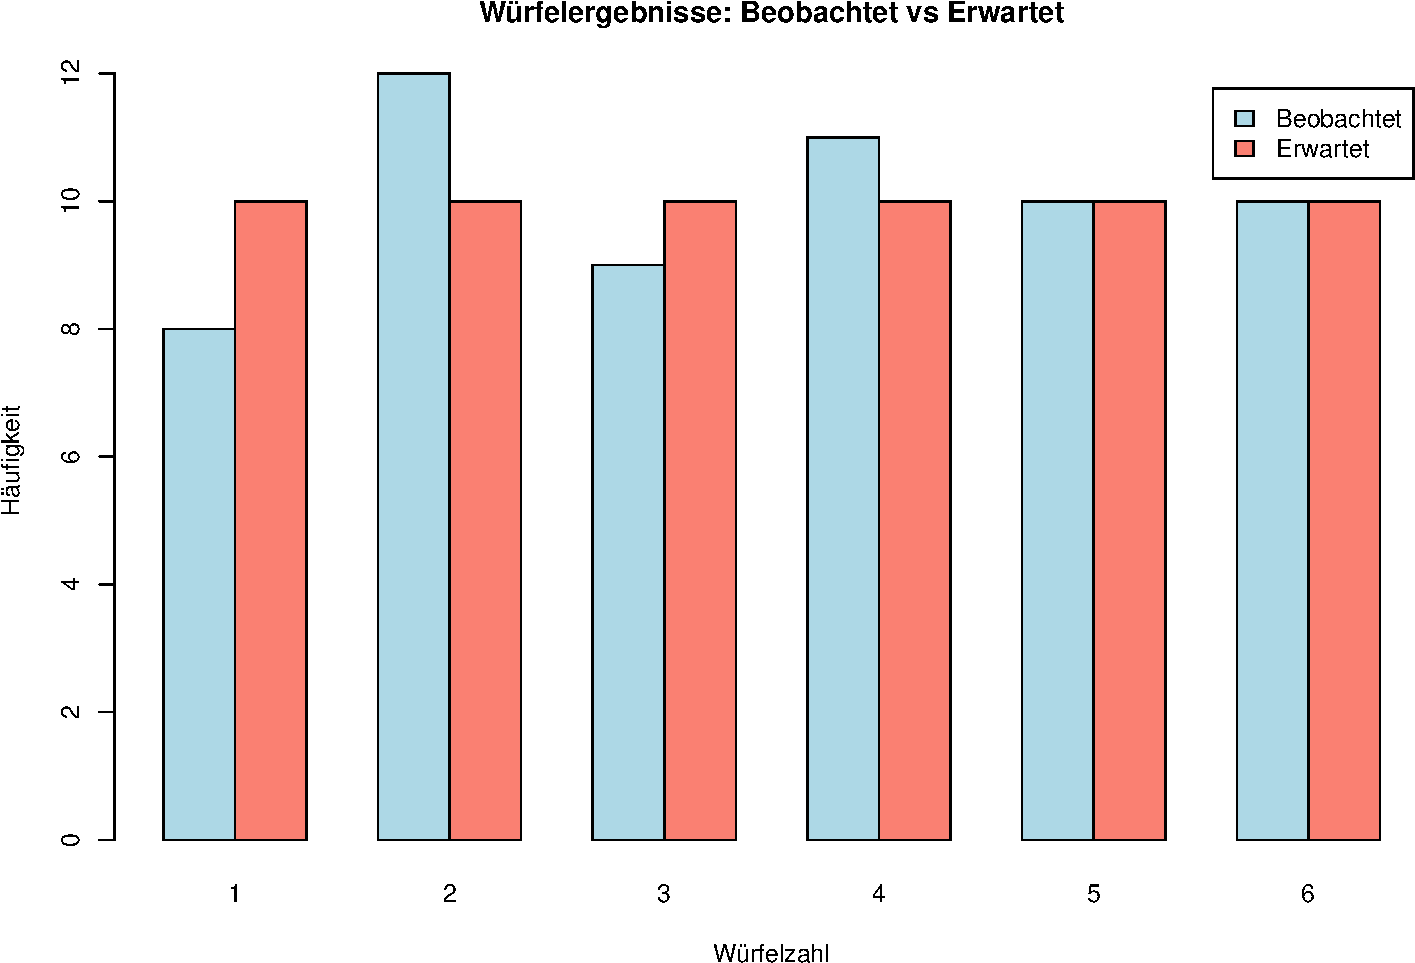
\includegraphics[keepaspectratio]{Statistik_Seminar_files/figure-beamer/unnamed-chunk-33-1.pdf}}
\end{frame}

\begin{frame}[fragile]{Chi-Quadrat-Test in R durchführen}
\protect\phantomsection\label{chi-quadrat-test-in-r-durchfuxfchren}
\begin{Shaded}
\begin{Highlighting}[]
\CommentTok{\# Automatischer Chi{-}Quadrat{-}Test}
\NormalTok{chi\_test }\OtherTok{\textless{}{-}} \FunctionTok{chisq.test}\NormalTok{(beobachtet)}

\CommentTok{\# Kompakte Ausgabe}
\FunctionTok{cat}\NormalTok{(}\StringTok{"χ² ="}\NormalTok{, chi\_test}\SpecialCharTok{$}\NormalTok{statistic, }
    \StringTok{"| df ="}\NormalTok{, chi\_test}\SpecialCharTok{$}\NormalTok{parameter, }
    \StringTok{"| p ="}\NormalTok{, }\FunctionTok{round}\NormalTok{(chi\_test}\SpecialCharTok{$}\NormalTok{p.value, }\DecValTok{4}\NormalTok{))}
\end{Highlighting}
\end{Shaded}

\begin{verbatim}
χ² = 1 | df = 5 | p = 0.9626
\end{verbatim}
\end{frame}

\begin{frame}{Freiheitsgrade verstehen}
\protect\phantomsection\label{freiheitsgrade-verstehen}
\begin{itemize}
\tightlist
\item
  \textbf{Formel für Anpassungstest}: df = Kategorien - 1 = 6 - 1 = 5
\item
  \textbf{Warum -1?}: Wenn 5 Häufigkeiten festgelegt sind, ist die 6.
  automatisch bestimmt
\item
  \textbf{Einfluss auf kritische Werte}: Mehr Freiheitsgrade → höhere
  kritische Werte
\end{itemize}
\end{frame}

\begin{frame}[fragile]{Freiheitsgrade verstehen}
\protect\phantomsection\label{freiheitsgrade-verstehen-1}
\begin{Shaded}
\begin{Highlighting}[]
\CommentTok{\# Kritische Werte anzeigen}
\FunctionTok{qchisq}\NormalTok{(}\FloatTok{0.95}\NormalTok{, }\AttributeTok{df =} \DecValTok{5}\NormalTok{)  }\CommentTok{\# 95\%{-}Quantil}
\end{Highlighting}
\end{Shaded}

\begin{verbatim}
[1] 11.0705
\end{verbatim}

\begin{Shaded}
\begin{Highlighting}[]
\FunctionTok{qchisq}\NormalTok{(}\FloatTok{0.99}\NormalTok{, }\AttributeTok{df =} \DecValTok{5}\NormalTok{)  }\CommentTok{\# 99\%{-}Quantil}
\end{Highlighting}
\end{Shaded}

\begin{verbatim}
[1] 15.08627
\end{verbatim}
\end{frame}

\begin{frame}{Arten von Chi-Quadrat-Tests}
\protect\phantomsection\label{arten-von-chi-quadrat-tests}
\begin{block}{1. Anpassungstest (Goodness-of-Fit)}
\protect\phantomsection\label{anpassungstest-goodness-of-fit}
\begin{itemize}
\tightlist
\item
  \textbf{Zweck}: Vergleich mit theoretischer Verteilung
\item
  \textbf{Beispiel}: Ist unser Würfel fair?
\item
  \textbf{H₀}: Alle Würfelseiten sind gleich wahrscheinlich
\item
  \textbf{H₁}: Mindestens eine Seite weicht ab
\end{itemize}
\end{block}
\end{frame}

\begin{frame}[fragile]{Unser Würfeltest}
\protect\phantomsection\label{unser-wuxfcrfeltest}
\begin{Shaded}
\begin{Highlighting}[]
\FunctionTok{chisq.test}\NormalTok{(beobachtet, }\AttributeTok{p =} \FunctionTok{rep}\NormalTok{(}\DecValTok{1}\SpecialCharTok{/}\DecValTok{6}\NormalTok{, }\DecValTok{6}\NormalTok{))}
\end{Highlighting}
\end{Shaded}

\begin{verbatim}

    Chi-squared test for given probabilities

data:  beobachtet
X-squared = 1, df = 5, p-value = 0.9626
\end{verbatim}
\end{frame}

\begin{frame}[fragile]{Arten von Chi-Quadrat-Tests}
\protect\phantomsection\label{arten-von-chi-quadrat-tests-1}
\begin{block}{2. Unabhängigkeitstest}
\protect\phantomsection\label{unabhuxe4ngigkeitstest}
\begin{itemize}
\tightlist
\item
  \textbf{Zweck}: Zusammenhang zwischen zwei kategorialen Variablen
\item
  \textbf{Beispiel}: Hängt die Würfelzahl vom Werfer ab?
\end{itemize}

\begin{verbatim}
      Würfelzahl
Person  1  2  3  4  5  6
     A  5  5  8  3  3  6
     B  0  3 10  6  4  7
\end{verbatim}
\end{block}
\end{frame}

\begin{frame}[fragile]{Unabhängigkeitstest durchführen}
\protect\phantomsection\label{unabhuxe4ngigkeitstest-durchfuxfchren}
\begin{verbatim}

    Pearson's Chi-squared test

data:  kontingenztab
X-squared = 6.942, df = 5, p-value = 0.225
\end{verbatim}
\end{frame}

\begin{frame}{Arten von Chi-Quadrat-Tests}
\protect\phantomsection\label{arten-von-chi-quadrat-tests-2}
\begin{block}{3. Homogenitätstest}
\protect\phantomsection\label{homogenituxe4tstest}
\begin{itemize}
\tightlist
\item
  \textbf{Zweck}: Vergleich von Verteilungen in verschiedenen Gruppen
\item
  \textbf{Beispiel}: Haben drei verschiedene Würfel die gleiche
  Verteilung?
\end{itemize}
\end{block}
\end{frame}

\begin{frame}{Voraussetzungen des Chi-Quadrat-Tests}
\protect\phantomsection\label{voraussetzungen-des-chi-quadrat-tests}
\begin{enumerate}
\tightlist
\item
  \textbf{Unabhängigkeit der Beobachtungen}

  \begin{itemize}
  \tightlist
  \item
    Jeder Würfelwurf unabhängig
  \item
    Keine wiederholten Messungen derselben Person
  \end{itemize}
\end{enumerate}
\end{frame}

\begin{frame}{Voraussetzungen des Chi-Quadrat-Tests}
\protect\phantomsection\label{voraussetzungen-des-chi-quadrat-tests-1}
\begin{enumerate}
\setcounter{enumi}{1}
\tightlist
\item
  \textbf{Erwartete Häufigkeiten ≥ 5}

  \begin{itemize}
  \tightlist
  \item
    In jeder Zelle der Tabelle
  \item
    Bei Verletzung: Kategorien zusammenfassen oder andere Tests
  \end{itemize}
\end{enumerate}
\end{frame}

\begin{frame}{Alternativen bei kleinen Stichproben: Fisher's Exakter
Test}
\protect\phantomsection\label{alternativen-bei-kleinen-stichproben-fishers-exakter-test}
\begin{itemize}
\tightlist
\item
  \textbf{Wann}: Erwartete Häufigkeiten \textless{} 5 in 2×2-Tabellen
\item
  \textbf{Vorteil}: Exakte p-Werte, keine Approximation
\end{itemize}
\end{frame}

\begin{frame}{Visualisierung kategorialer Daten}
\protect\phantomsection\label{visualisierung-kategorialer-daten}
\pandocbounded{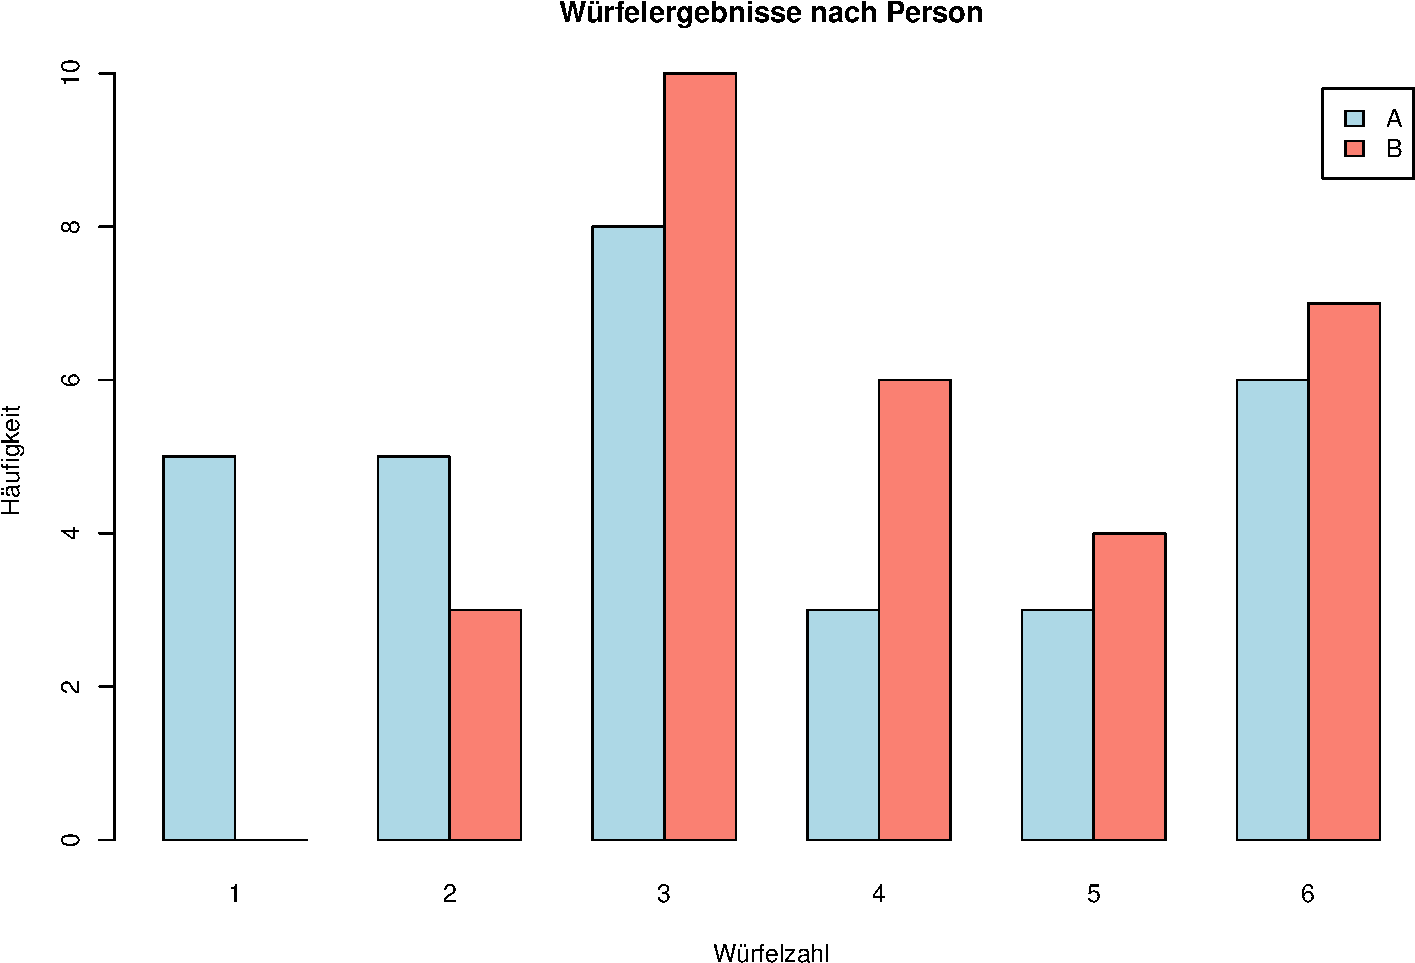
\includegraphics[keepaspectratio]{Statistik_Seminar_files/figure-beamer/unnamed-chunk-39-1.pdf}}
\end{frame}

\begin{frame}{Mosaikplots}
\protect\phantomsection\label{mosaikplots}
\pandocbounded{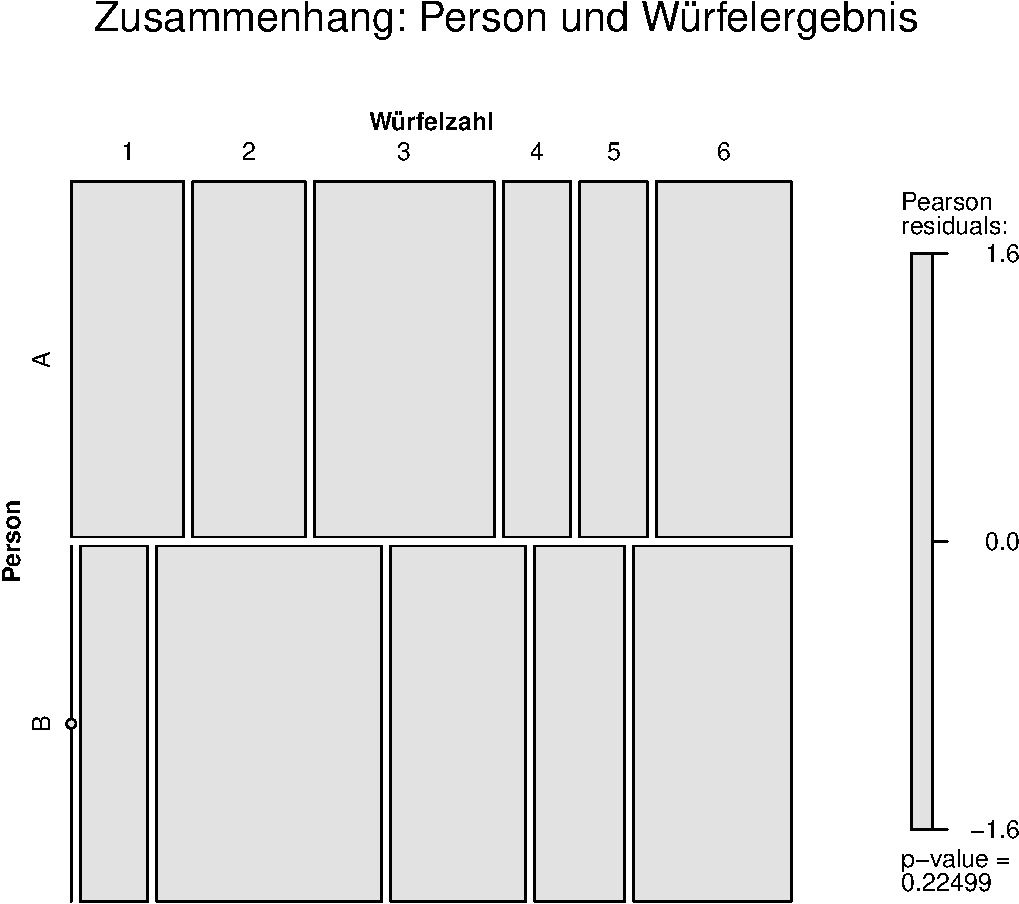
\includegraphics[keepaspectratio]{Statistik_Seminar_files/figure-beamer/unnamed-chunk-40-1.pdf}}
\end{frame}

\begin{frame}{Praktische Anwendungsbeispiele}
\protect\phantomsection\label{praktische-anwendungsbeispiele-1}
\begin{block}{Marktforschung}
\protect\phantomsection\label{marktforschung}
\begin{itemize}
\tightlist
\item
  \textbf{Frage}: Bevorzugen verschiedene Altersgruppen unterschiedliche
  Produktfarben?
\item
  \textbf{Test}: Unabhängigkeitstest (Alter × Farbpräferenz)
\end{itemize}
\end{block}

\begin{block}{Medizin}
\protect\phantomsection\label{medizin}
\begin{itemize}
\tightlist
\item
  \textbf{Frage}: Ist ein neues Medikament wirksam?
\item
  \textbf{Test}: Unabhängigkeitstest (Behandlung × Heilung)
\end{itemize}
\end{block}
\end{frame}

\begin{frame}{Praktische Anwendungsbeispiele}
\protect\phantomsection\label{praktische-anwendungsbeispiele-2}
\begin{block}{Qualitätskontrolle}
\protect\phantomsection\label{qualituxe4tskontrolle}
\begin{itemize}
\tightlist
\item
  \textbf{Frage}: Produziert eine Maschine gleichmäßig?
\item
  \textbf{Test}: Anpassungstest (beobachtete vs erwartete
  Produktverteilung)
\end{itemize}
\end{block}
\end{frame}

\begin{frame}{TEIL 2: Vertiefung - Residuenanalyse und Effektstärken}
\protect\phantomsection\label{teil-2-vertiefung---residuenanalyse-und-effektstuxe4rken}
\textbf{Problem der bisherigen Analyse:}

\begin{itemize}
\tightlist
\item
  Chi-Quadrat-Test sagt nur ``es gibt einen Unterschied''
\item
  \textbf{Aber nicht:} Wo? Wie stark? Praktisch relevant?
\end{itemize}

\textbf{Lösung:}

\begin{itemize}
\tightlist
\item
  \textbf{Residuenanalyse}: Wo sind die Unterschiede?
\item
  \textbf{Effektstärken}: Wie stark sind sie?
\end{itemize}
\end{frame}

\begin{frame}{Residuenanalyse: Die Grundlagen}
\protect\phantomsection\label{residuenanalyse-die-grundlagen}
\textbf{Das Problem:} Chi-Quadrat-Test sagt nur ``es gibt einen
Unterschied''

\textbf{Die Lösung:} Residuen zeigen \textbf{wo} die Unterschiede liegen

\textbf{Was sind Residuen?}

\begin{itemize}
\tightlist
\item
  \textbf{Residuen}: \(r = O - E\) (Beobachtet - Erwartet)
\item
  \textbf{Problem der Residuen}: Schwer zu interpretieren (ist +3 viel
  oder wenig?)
\item
  \textbf{Lösung}: Standardisierte Residuen - vergleichbar zwischen
  verschiedenen Zellen
\end{itemize}
\end{frame}

\begin{frame}{Von Residuen zu standardisierten Residuen}
\protect\phantomsection\label{von-residuen-zu-standardisierten-residuen}
\begin{columns}[T]
\begin{column}{0.5\linewidth}
\textbf{Rohresiduen-Problem:}

\begin{itemize}
\tightlist
\item
  Zelle A: +3 (von erwartet 10)
\item
  Zelle B: +3 (von erwartet 100)
\item
  Gleiche Abweichung, aber sehr unterschiedliche Bedeutung!
\end{itemize}
\end{column}

\begin{column}{0.5\linewidth}
\textbf{Standardisierte Residuen:} \(sr = \frac{O - E}{\sqrt{E}}\)

\begin{itemize}
\tightlist
\item
  Berücksichtigen die ``natürliche'' Schwankung
\item
  Werden vergleichbar zwischen Zellen
\item
  Größere erwartete Werte → größere natürliche Schwankung
\end{itemize}
\end{column}
\end{columns}
\end{frame}

\begin{frame}{Standardisierte Residuen verstehen}
\protect\phantomsection\label{standardisierte-residuen-verstehen}
\textbf{Intuitive Interpretation:}

\begin{itemize}
\tightlist
\item
  \textbf{sr = 0}: Genau wie erwartet
\item
  \textbf{sr = +1}: Ein bisschen mehr als erwartet
\item
  \textbf{sr = +2}: Deutlich mehr als erwartet
\item
  \textbf{sr = +3}: Sehr viel mehr als erwartet
\end{itemize}
\end{frame}

\begin{frame}{Standardisierte Residuen verstehen}
\protect\phantomsection\label{standardisierte-residuen-verstehen-1}
\textbf{Interpretationsrichtlinien:}

\begin{itemize}
\tightlist
\item
  \(|sr| < 2\): Noch im normalen Bereich der Zufallsschwankung
\item
  \(|sr| > 2\): Ungewöhnlich - vermutlich nicht nur Zufall
\item
  \(|sr| > 3\): Sehr ungewöhnlich - fast sicher nicht nur Zufall
\end{itemize}

\textbf{Vorzeichen:}

\begin{itemize}
\tightlist
\item
  \textbf{Positiv (+)}: Mehr als erwartet
\item
  \textbf{Negativ (-)}: Weniger als erwartet
\end{itemize}
\end{frame}

\begin{frame}{Das Problem mit p-Werten}
\protect\phantomsection\label{das-problem-mit-p-werten}
\begin{columns}[T]
\begin{column}{0.5\linewidth}
\textbf{p-Wert beantwortet nur:}

\begin{itemize}
\tightlist
\item
  Gibt es einen Effekt?'' (Ja/Nein)
\item
  Wird bei großen Stichproben fast immer signifikant
\end{itemize}

\textbf{p-Wert sagt NICHT:}

\begin{itemize}
\tightlist
\item
  Wie stark ist der Effekt?
\item
  Ist der Effekt praktisch relevant?
\end{itemize}
\end{column}

\begin{column}{0.5\linewidth}
\textbf{Beispiel Problem:}

\begin{itemize}
\tightlist
\item
  10.000 Personen
\item
  Winziger, praktisch irrelevanter Unterschied
\item
  Trotzdem p \textless{} 0.001
\item
  \textbf{Ohne Effektstärke:} Fehlinterpretation!
\end{itemize}
\end{column}
\end{columns}
\end{frame}

\begin{frame}{Effektstärken: Die Lösung}
\protect\phantomsection\label{effektstuxe4rken-die-luxf6sung}
\textbf{Cramér's V} - Die wichtigste Effektstärke für Chi-Quadrat-Tests

\textbf{Formel:} \[V = \sqrt{\frac{\chi^2}{n \times (\min(r,c) - 1)}}\]

Wo:

\begin{itemize}
\tightlist
\item
  n = Gesamtstichprobengröße
\item
  r = Anzahl Zeilen
\item
  c = Anzahl Spalten
\end{itemize}
\end{frame}

\begin{frame}{Cramér's V interpretieren}
\protect\phantomsection\label{cramuxe9rs-v-interpretieren}
\begin{columns}[T]
\begin{column}{0.5\linewidth}
\textbf{Interpretationsrichtlinien:}

\begin{itemize}
\tightlist
\item
  \textbf{0.00 - 0.10}: Vernachlässigbarer Effekt
\item
  \textbf{0.10 - 0.30}: Kleiner Effekt
\item
  \textbf{0.30 - 0.50}: Mittlerer Effekt
\item
  \textbf{0.50+}: Großer Effekt
\end{itemize}
\end{column}

\begin{column}{0.5\linewidth}
\textbf{Wichtig:}

\begin{itemize}
\tightlist
\item
  Unabhängig von Stichprobengröße
\item
  Vergleichbar zwischen Studien
\item
  Standardisiert zwischen 0 und 1
\end{itemize}
\end{column}
\end{columns}
\end{frame}

\begin{frame}{Weitere Effektstärken für 2×2-Tabellen}
\protect\phantomsection\label{weitere-effektstuxe4rken-fuxfcr-22-tabellen}
\begin{block}{Phi-Koeffizient (φ)}
\protect\phantomsection\label{phi-koeffizient-ux3c6}
\textbf{Nur für 2×2-Tabellen:} φ = √(χ² / n)
\end{block}

\begin{block}{Odds Ratio (OR)}
\protect\phantomsection\label{odds-ratio-or}
\textbf{Interpretation:} Um wie viel mal wahrscheinlicher ist ein
Ereignis in Gruppe A vs.~B?
\end{block}
\end{frame}

\begin{frame}{APA-konformes Berichten}
\protect\phantomsection\label{apa-konformes-berichten}
\textbf{Vollständiger Bericht:}

\emph{``Ein Chi-Quadrat-Unabhängigkeitstest zeigte einen signifikanten
Zusammenhang zwischen Geschlecht und Studienfachwahl, χ²(2) = 8.24, p =
.016, Cramér's V = .23. Die Residuenanalyse ergab, dass Männer in den
Sozialwissenschaften überrepräsentiert waren (sr = 2.68), während Frauen
in MINT-Fächern häufiger vertreten waren als erwartet (sr = 1.58).''}
\end{frame}

\begin{frame}{Häufige Fehler vermeiden}
\protect\phantomsection\label{huxe4ufige-fehler-vermeiden}
\begin{block}{❌ Falsche Annahmen:}
\protect\phantomsection\label{falsche-annahmen}
\begin{itemize}
\tightlist
\item
  Kontinuierliche Daten kategorisieren nur für Chi-Quadrat-Test
\item
  ``Großes χ² bedeutet automatisch wichtigen Effekt''
\item
  ``Signifikanz = praktische Bedeutsamkeit''
\item
  Erwartete Häufigkeiten \textless{} 5 ignorieren
\end{itemize}
\end{block}
\end{frame}

\begin{frame}{Häufige Fehler vermeiden}
\protect\phantomsection\label{huxe4ufige-fehler-vermeiden-1}
\begin{block}{✅ Richtige Interpretation:}
\protect\phantomsection\label{richtige-interpretation}
\begin{itemize}
\tightlist
\item
  \textbf{Signifikanz UND Effektstärke} zusammen betrachten
\item
  Angemessene Teststärke durch ausreichende Stichproben
\item
  Voraussetzungen prüfen
\item
  \textbf{Residuen für detaillierte Analyse nutzen}
\end{itemize}
\end{block}
\end{frame}

\begin{frame}{Nicht immer ist es ein Chi Square-Test}
\protect\phantomsection\label{nicht-immer-ist-es-ein-chi-square-test}
``The trial enrolled 30,420 volunteers who were randomly assigned in a
1:1 ratio to receive either vaccine or placebo (15,210 participants in
each group). More than 96\% of participants received both injections
{[}\ldots{]}. Symptomatic Covid-19 illness was confirmed in 185
participants in the placebo group (56.5 per 1000 person-years; 95\%
confidence interval {[}CI{]}, 48.7 to 65.3) and in 11 participants in
the mRNA-1273 group (3.3 per 1000 person-years; 95\% CI, 1.7 to 6.0);
vaccine efficacy was 94.1\% (95\% CI, 89.3 to 96.8\%;
P\textless0.001).''
\end{frame}

\section{Sitzung 9:
Korrelationsanalyse}\label{sitzung-9-korrelationsanalyse}

\begin{frame}{Lernziele dieser Sitzung}
\protect\phantomsection\label{lernziele-dieser-sitzung-7}
\begin{itemize}
\tightlist
\item
  Korrelation von Kausalität unterscheiden
\item
  Pearson-, Spearman- und Kendall-Korrelation situationsgerecht
  einsetzen
\item
  Korrelationsmatrizen erstellen und interpretieren
\item
  Typische Fallstricke (Scheinkorrelation, Simpson's Paradoxon) erkennen
\end{itemize}
\end{frame}

\begin{frame}{Was ist eine Korrelation?}
\protect\phantomsection\label{was-ist-eine-korrelation}
\pandocbounded{\includegraphics[keepaspectratio]{images/1840_bachelors-degrees-awarded-in-library-science_correlates-with_google-searches-for-how-to-hide-a-body.png}}
\end{frame}

\begin{frame}{Was war zuerst da?}
\protect\phantomsection\label{was-war-zuerst-da}
\pandocbounded{\includegraphics[keepaspectratio]{images/murder.png}}
\end{frame}

\begin{frame}{Grundkonzepte der Korrelation}
\protect\phantomsection\label{grundkonzepte-der-korrelation}
\begin{itemize}
\tightlist
\item
  \textbf{Definition}: Stärke eines Zusammenhangs zwischen Variablen
\item
  \textbf{Unterschied zu Kausalität}: Korrelation impliziert keine
  Ursache-Wirkung-Beziehung
\end{itemize}
\end{frame}

\begin{frame}{Von der Kovarianz zur Korrelation}
\protect\phantomsection\label{von-der-kovarianz-zur-korrelation}
\begin{itemize}
\tightlist
\item
  \textbf{Kovarianz}: Unstandartisiertes Maß für gemeinsame Variation

  \begin{itemize}
  \tightlist
  \item
    Formel:
    \(\text{Cov}(X,Y) = \frac{1}{n-1} \sum_{i=1}^{n} (x_i - \bar{x})(y_i - \bar{y})\)
  \end{itemize}
\item
  \textbf{Pearson-Korrelation}: Standardisierte Kovarianz

  \begin{itemize}
  \tightlist
  \item
    Formel: \(r = \frac{\text{Cov}(X,Y)}{s_X \cdot s_Y}\)
  \item
    Wertebereich: -1 bis +1
  \end{itemize}
\end{itemize}
\end{frame}

\begin{frame}[fragile]{Pearson-Korrelation}
\protect\phantomsection\label{pearson-korrelation}
\begin{itemize}
\item
  \textbf{Voraussetzungen}:

  \begin{itemize}
  \tightlist
  \item
    Lineare Beziehung
  \item
    Normalverteilung der Variablen (für Hypothesentests)
  \item
    Keine Ausreißer (starker Einfluss auf r)
  \end{itemize}
\item
  \textbf{Interpretation der Stärke}:

  \begin{itemize}
  \tightlist
  \item
    Schwach: \textbar r\textbar{} ≈ 0.1-0.3
  \item
    Mittel: \textbar r\textbar{} ≈ 0.3-0.5
  \item
    Stark: \textbar r\textbar{} \textgreater{} 0.5
  \end{itemize}
\item
  R-Code: \texttt{cor.test(daten\$x,\ daten\$y)}
\end{itemize}
\end{frame}

\begin{frame}{Visualisierung: Streudiagramm}
\protect\phantomsection\label{visualisierung-streudiagramm}
\pandocbounded{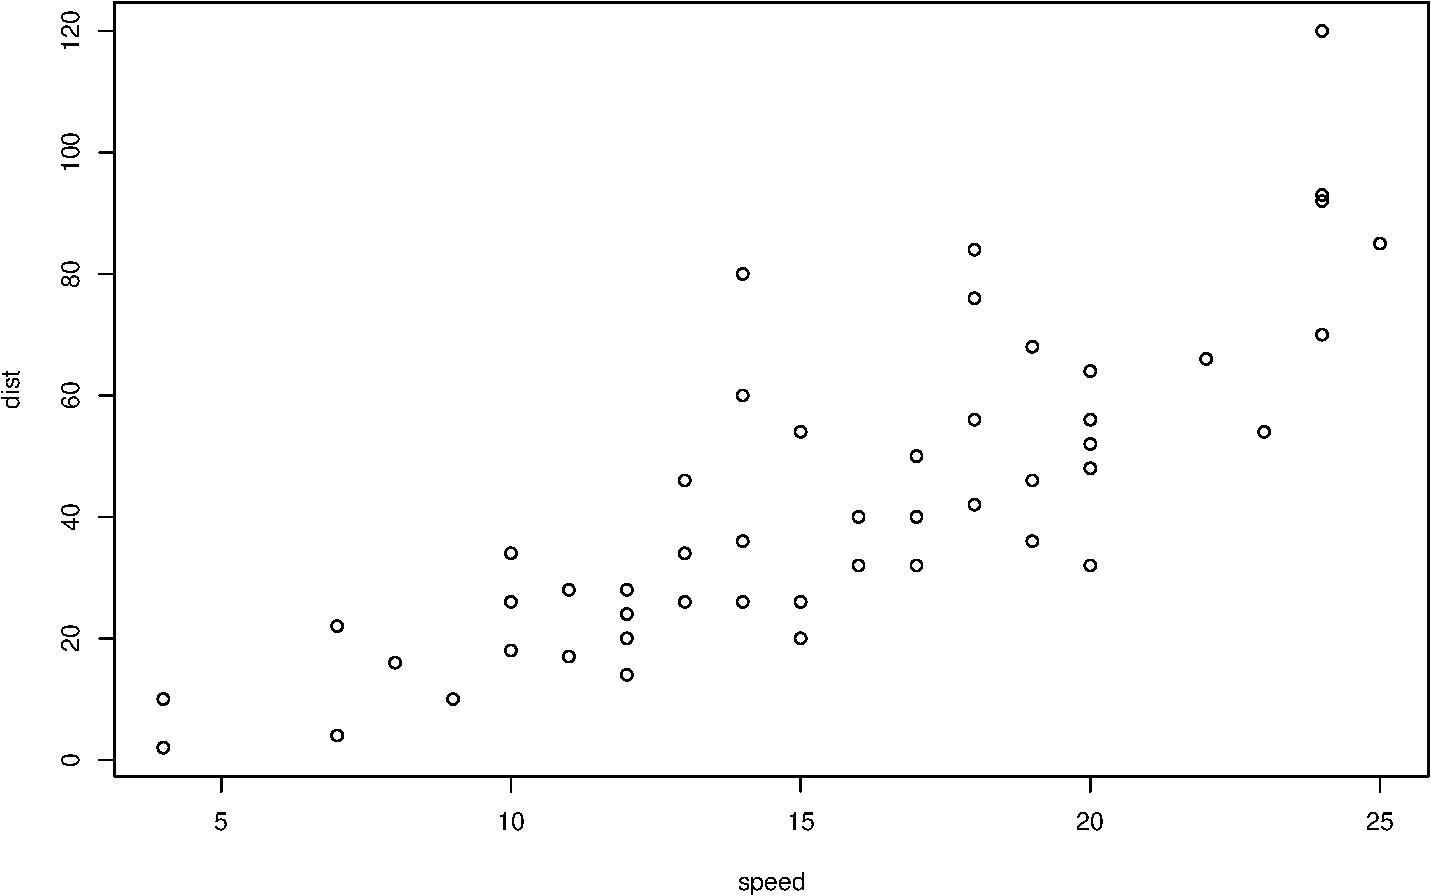
\includegraphics[keepaspectratio]{Statistik_Seminar_files/figure-beamer/unnamed-chunk-41-1.pdf}}
\end{frame}

\begin{frame}{Durchführung in R}
\protect\phantomsection\label{durchfuxfchrung-in-r}
\pandocbounded{\includegraphics[keepaspectratio]{images/pearson.png}}
\end{frame}

\begin{frame}[fragile]{Alternative Korrelationsmaße}
\protect\phantomsection\label{alternative-korrelationsmauxdfe}
\begin{itemize}
\tightlist
\item
  \textbf{Spearman-Rangkorrelation}: Für ordinale Daten oder
  nicht-lineare monotone Beziehungen

  \begin{itemize}
  \tightlist
  \item
    Formel: Pearson-Korrelation der rangtransformierten Daten
  \item
    Robuster gegenüber Ausreißern
  \item
    R-Code:
    \texttt{cor.test(daten\$x,\ daten\$y,\ method\ =\ "spearman")}
  \end{itemize}
\end{itemize}
\end{frame}

\begin{frame}[fragile]{Alternative Korrelationsmaße}
\protect\phantomsection\label{alternative-korrelationsmauxdfe-1}
\begin{itemize}
\tightlist
\item
  \textbf{Kendall's Tau}: Alternative rangbasierte Korrelation

  \begin{itemize}
  \tightlist
  \item
    Basiert auf konkordanten vs.~diskordanten Paaren
  \item
    Robuster bei kleinen Stichproben
  \item
    R-Code:
    \texttt{cor.test(daten\$x,\ daten\$y,\ method\ =\ "kendall")}
  \end{itemize}
\end{itemize}
\end{frame}

\begin{frame}{Visualisierung: Korrelationsmatrix}
\protect\phantomsection\label{visualisierung-korrelationsmatrix}
\pandocbounded{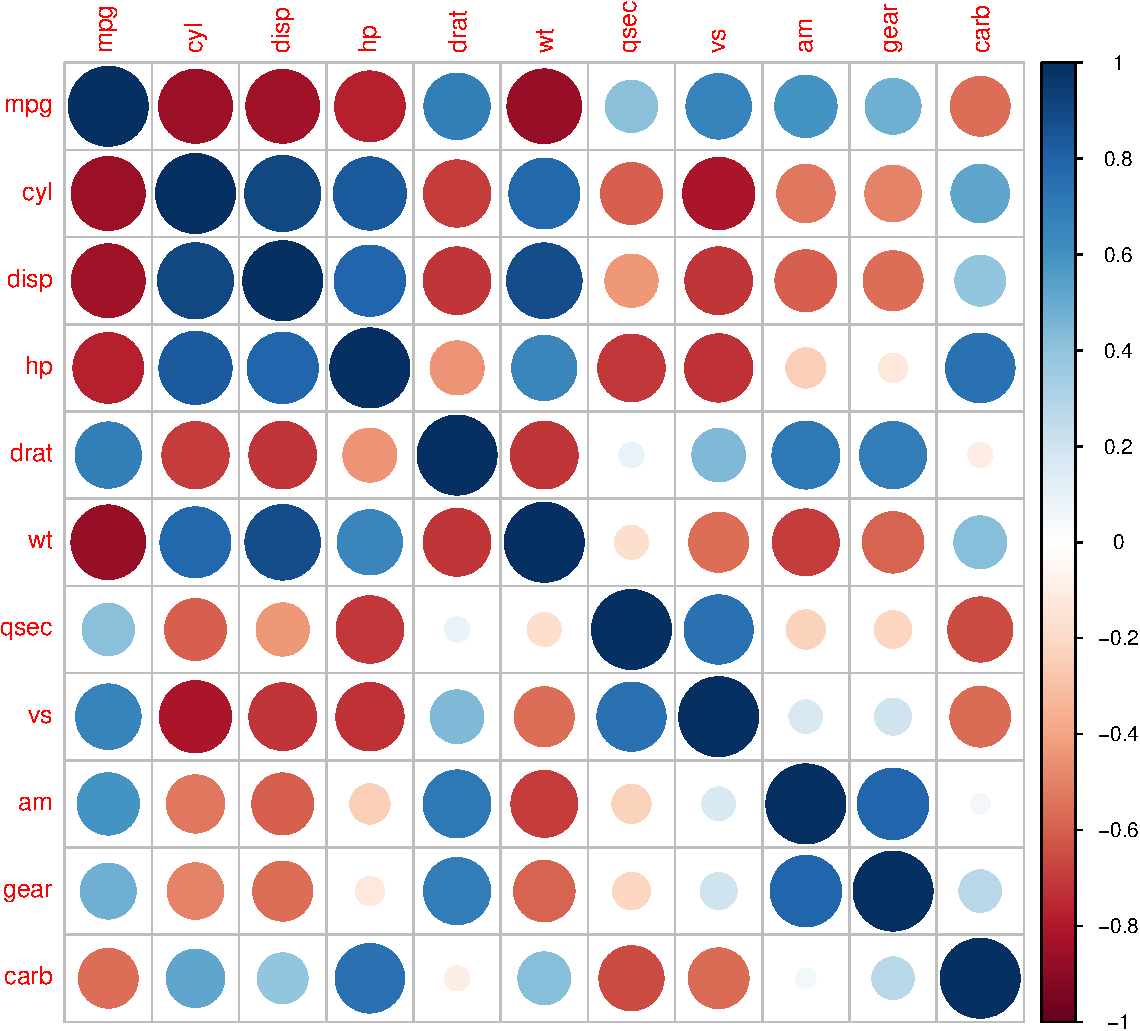
\includegraphics[keepaspectratio]{Statistik_Seminar_files/figure-beamer/unnamed-chunk-42-1.pdf}}
\end{frame}

\begin{frame}{Fallstricke und Fehlinterpretationen}
\protect\phantomsection\label{fallstricke-und-fehlinterpretationen}
\begin{itemize}
\tightlist
\item
  \textbf{Scheinkorrelationen}: Effekt von Drittvariablen
\item
  \textbf{Nichtlineare Beziehungen}: Wenn r = 0 trotz starkem
  Zusammenhang
\item
  \textbf{Aggregationsprobleme}: Simpson's Paradoxon
\item
  \textbf{Extremwerte und Ausreißer}: Starker Einfluss auf die
  Korrelation
\end{itemize}
\end{frame}

\begin{frame}{Simpson's Paradoxon: Studienplatzvergabe}
\protect\phantomsection\label{simpsons-paradoxon-studienplatzvergabe}
{\def\LTcaptype{none} % do not increment counter
\begin{longtable}[]{@{}llll@{}}
\toprule\noalign{}
Geschlecht & Bewerbungen & Zugelassen & Annahmequote \\
\midrule\noalign{}
\endhead
Männer & 1000 & 600 & 60\% \\
Frauen & 1000 & 500 & 50\% \\
\bottomrule\noalign{}
\end{longtable}
}
\end{frame}

\begin{frame}{Simpson's Paradoxon: Studienplatzvergabe}
\protect\phantomsection\label{simpsons-paradoxon-studienplatzvergabe-1}
{\def\LTcaptype{none} % do not increment counter
\begin{longtable}[]{@{}
  >{\raggedright\arraybackslash}p{(\linewidth - 8\tabcolsep) * \real{0.3200}}
  >{\raggedright\arraybackslash}p{(\linewidth - 8\tabcolsep) * \real{0.1600}}
  >{\raggedright\arraybackslash}p{(\linewidth - 8\tabcolsep) * \real{0.1733}}
  >{\raggedright\arraybackslash}p{(\linewidth - 8\tabcolsep) * \real{0.1600}}
  >{\raggedright\arraybackslash}p{(\linewidth - 8\tabcolsep) * \real{0.1867}}@{}}
\toprule\noalign{}
\begin{minipage}[b]{\linewidth}\raggedright
Fach
\end{minipage} & \begin{minipage}[b]{\linewidth}\raggedright
Geschlecht
\end{minipage} & \begin{minipage}[b]{\linewidth}\raggedright
Bewerbungen
\end{minipage} & \begin{minipage}[b]{\linewidth}\raggedright
Zugelassen
\end{minipage} & \begin{minipage}[b]{\linewidth}\raggedright
Annahmequote
\end{minipage} \\
\midrule\noalign{}
\endhead
\textbf{Fach A (leicht)} & Männer & 800 & 560 & 70\% \\
& Frauen & 200 & 180 & 90\% \\
\textbf{Fach B (schwierig)} & Männer & 200 & 40 & 20\% \\
& Frauen & 800 & 320 & 40\% \\
\bottomrule\noalign{}
\end{longtable}
}
\end{frame}

\begin{frame}{Fallbeispiel: Kriminalität in NYC}
\protect\phantomsection\label{fallbeispiel-kriminalituxe4t-in-nyc}
\pandocbounded{\includegraphics[keepaspectratio]{images/Giuliani_crime_rate.png}}
\end{frame}

\begin{frame}{Wurden die Verbrecher erst gar nicht geboren?}
\protect\phantomsection\label{wurden-die-verbrecher-erst-gar-nicht-geboren}
\pandocbounded{\includegraphics[keepaspectratio]{images/baby_pill.png}}
\end{frame}

\begin{frame}{War es das Blei im Benzin?}
\protect\phantomsection\label{war-es-das-blei-im-benzin}
\pandocbounded{\includegraphics[keepaspectratio]{images/blog_lead_crime_main_chart.png}}
\end{frame}

\begin{frame}{Was war es denn nun?}
\protect\phantomsection\label{was-war-es-denn-nun}
\pandocbounded{\includegraphics[keepaspectratio]{images/change_my_mind.png}}
\end{frame}

\begin{frame}{Inter-Rater Reliability}
\protect\phantomsection\label{inter-rater-reliability}
\begin{itemize}
\item
  \textbf{Definition}: Konsistenz zwischen verschiedenen Beurteilern
\item
  \textbf{Anwendungsbereiche}: Subjektive Bewertungen, medizinische
  Diagnosen, Content-Analysen
\item
  \textbf{Maße für kategoriale Daten}:

  \begin{itemize}
  \tightlist
  \item
    Cohen's Kappa (zwei Rater)
  \item
    Fleiss' Kappa (mehr als zwei Rater)
  \end{itemize}
\item
  \textbf{Maße für kontinuierliche Daten}:

  \begin{itemize}
  \tightlist
  \item
    Intraclass Correlation Coefficient (ICC)
  \end{itemize}
\end{itemize}
\end{frame}

\begin{frame}{Visualisierung: Violinen-Diagramm}
\protect\phantomsection\label{visualisierung-violinen-diagramm}
\pandocbounded{\includegraphics[keepaspectratio]{images/spinaliom-vergleich-therapie.png}}
\end{frame}

\begin{frame}{Wann nutze ich eigentlich was?}
\protect\phantomsection\label{wann-nutze-ich-eigentlich-was}
\pandocbounded{\includegraphics[keepaspectratio]{images/entscheidungsbaum.png}}
\end{frame}

\section{Sitzung 10: Regression I -- Lineare
Regression}\label{sitzung-10-regression-i-lineare-regression}

\begin{frame}{Lernziele dieser Sitzung}
\protect\phantomsection\label{lernziele-dieser-sitzung-8}
\begin{itemize}
\tightlist
\item
  Ein lineares Regressionsmodell in R schätzen und interpretieren
\item
  R² und Residuenplots zur Modellbeurteilung nutzen
\item
  Multiple Regression mit kategorialen Prädiktoren anwenden
\item
  Den Unterschied zwischen Korrelation und Regression erklären
\end{itemize}
\end{frame}

\begin{frame}{Einstieg: Wie viel Miete ist zu viel?}
\protect\phantomsection\label{einstieg-wie-viel-miete-ist-zu-viel}
Sie wollen nach Berlin ziehen und finden 100 Wohnungsanzeigen. Dort
stehen jeweils Wohnfläche (qm) und Miete (Euro). \textgreater{}
\textgreater{} \textbf{Frage:} Kann man aus der Wohnfläche den Mietpreis
vorhersagen?
\end{frame}

\begin{frame}{Erste Visualisierung: Streudiagramm}
\protect\phantomsection\label{erste-visualisierung-streudiagramm}
\pandocbounded{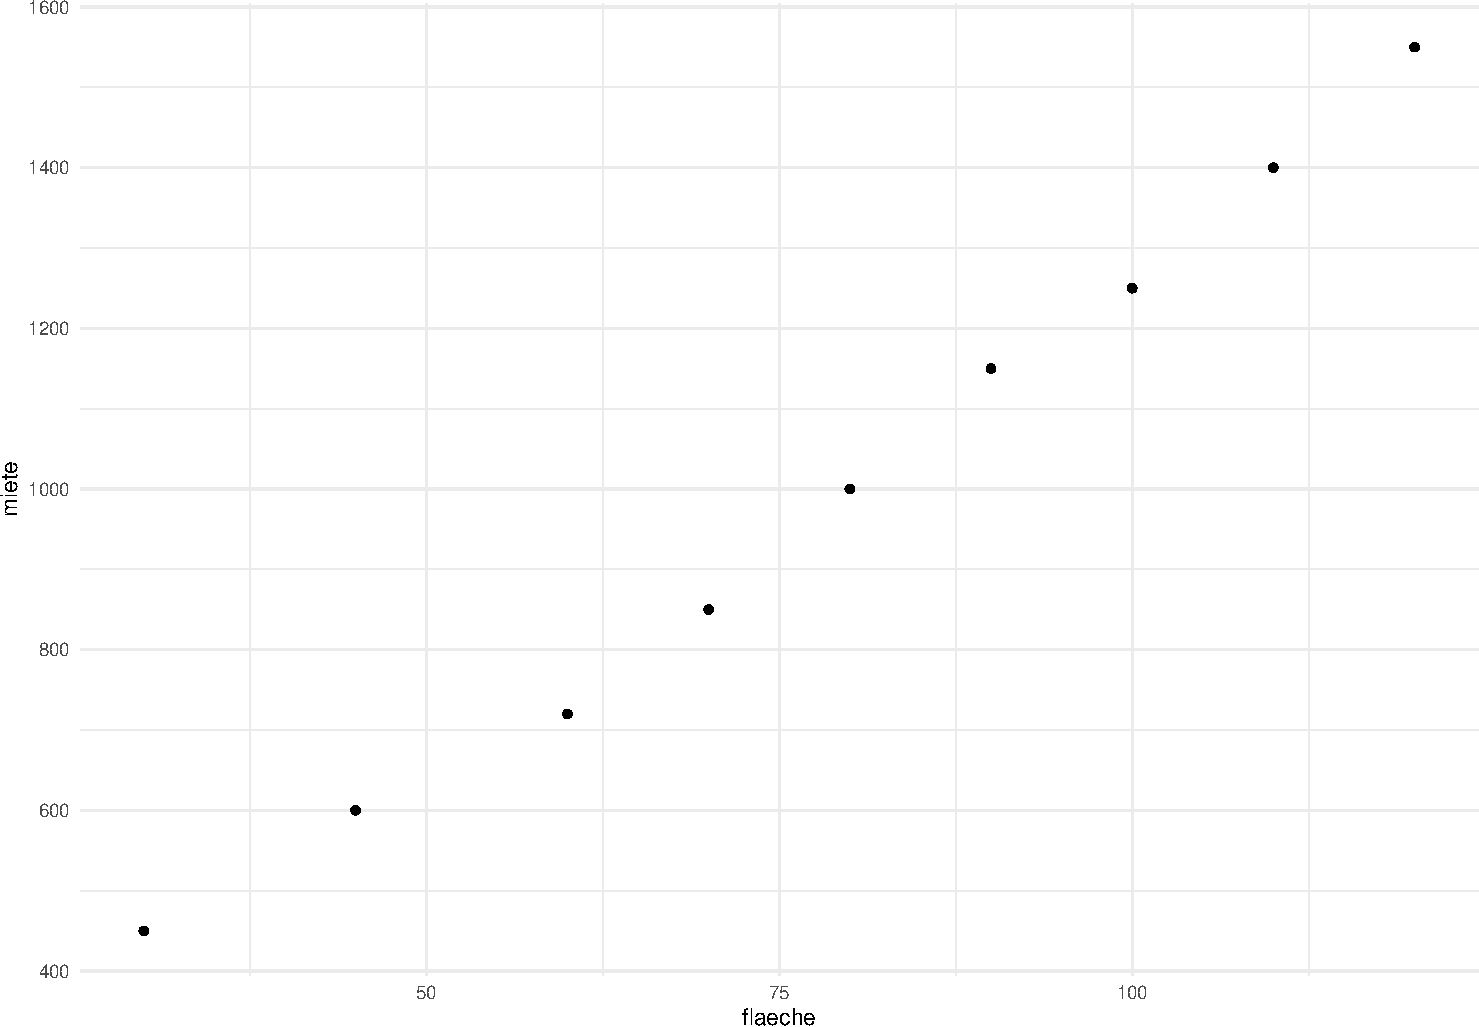
\includegraphics[keepaspectratio]{Statistik_Seminar_files/figure-beamer/unnamed-chunk-43-1.pdf}}
\end{frame}

\begin{frame}{Das Modell dahinter: Lineare Regression}
\protect\phantomsection\label{das-modell-dahinter-lineare-regression}
\[\hat{Y} = \beta_0 + \beta_1 \cdot X + \varepsilon\]

\begin{itemize}
\tightlist
\item
  \(\beta_0\): Startwert (Y bei X = 0)
\item
  \(\beta_1\): Steigung (Zunahme von Y bei 1 Einheit mehr X)
\item
  \(\varepsilon\): ``Fehler'' -- das, was das Modell nicht erklärt
\end{itemize}
\end{frame}

\begin{frame}
\pandocbounded{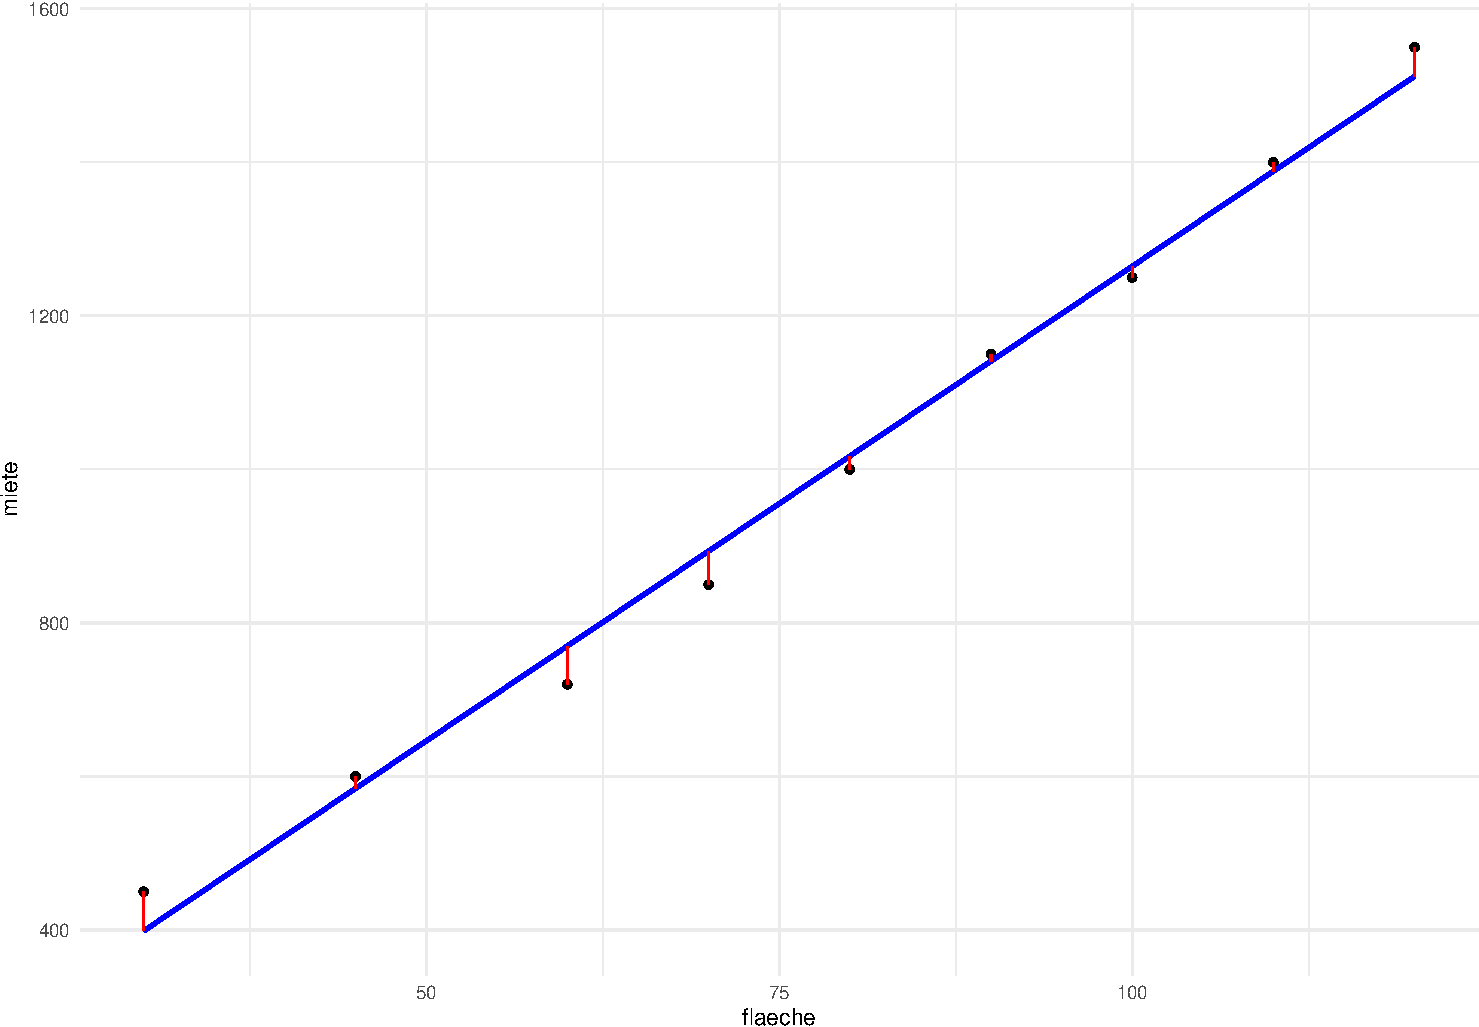
\includegraphics[keepaspectratio]{Statistik_Seminar_files/figure-beamer/unnamed-chunk-44-1.pdf}}
\end{frame}

\begin{frame}{Wie es genau funktioniert}
\protect\phantomsection\label{wie-es-genau-funktioniert}
\pandocbounded{\includegraphics[keepaspectratio]{images/linear_regression.gif}}
\end{frame}

\begin{frame}{Zweite Visualisierung: Streudiagramm mit Regressionslinie}
\protect\phantomsection\label{zweite-visualisierung-streudiagramm-mit-regressionslinie}
\pandocbounded{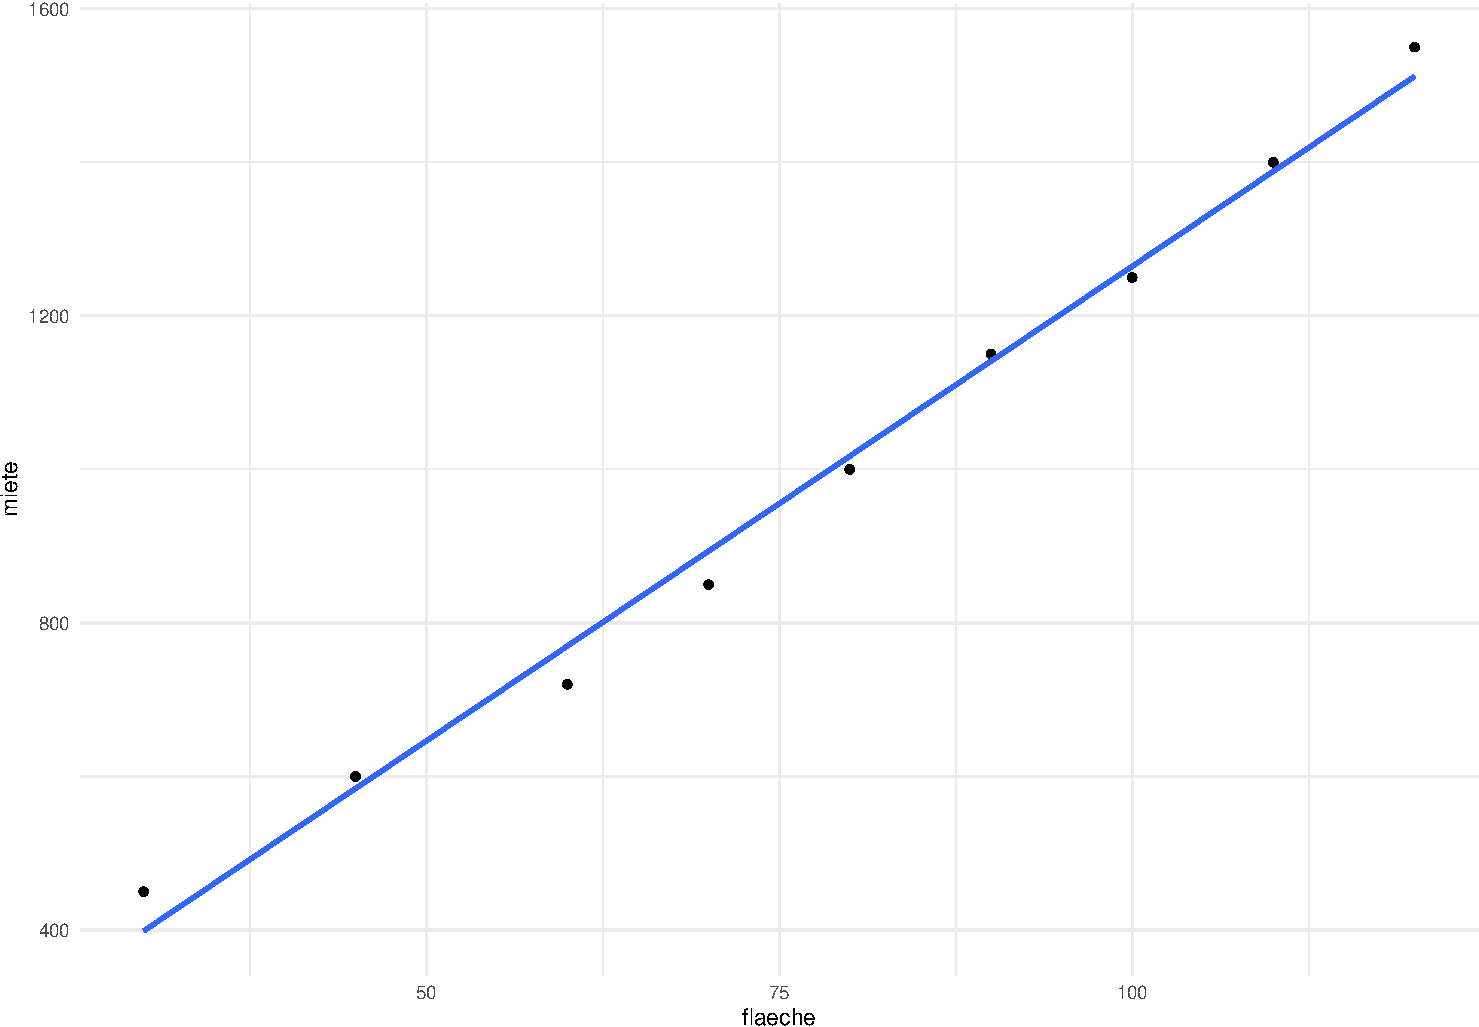
\includegraphics[keepaspectratio]{Statistik_Seminar_files/figure-beamer/unnamed-chunk-45-1.pdf}}
\end{frame}

\begin{frame}{R-Code zur Modellschätzung}
\protect\phantomsection\label{r-code-zur-modellschuxe4tzung}
\pandocbounded{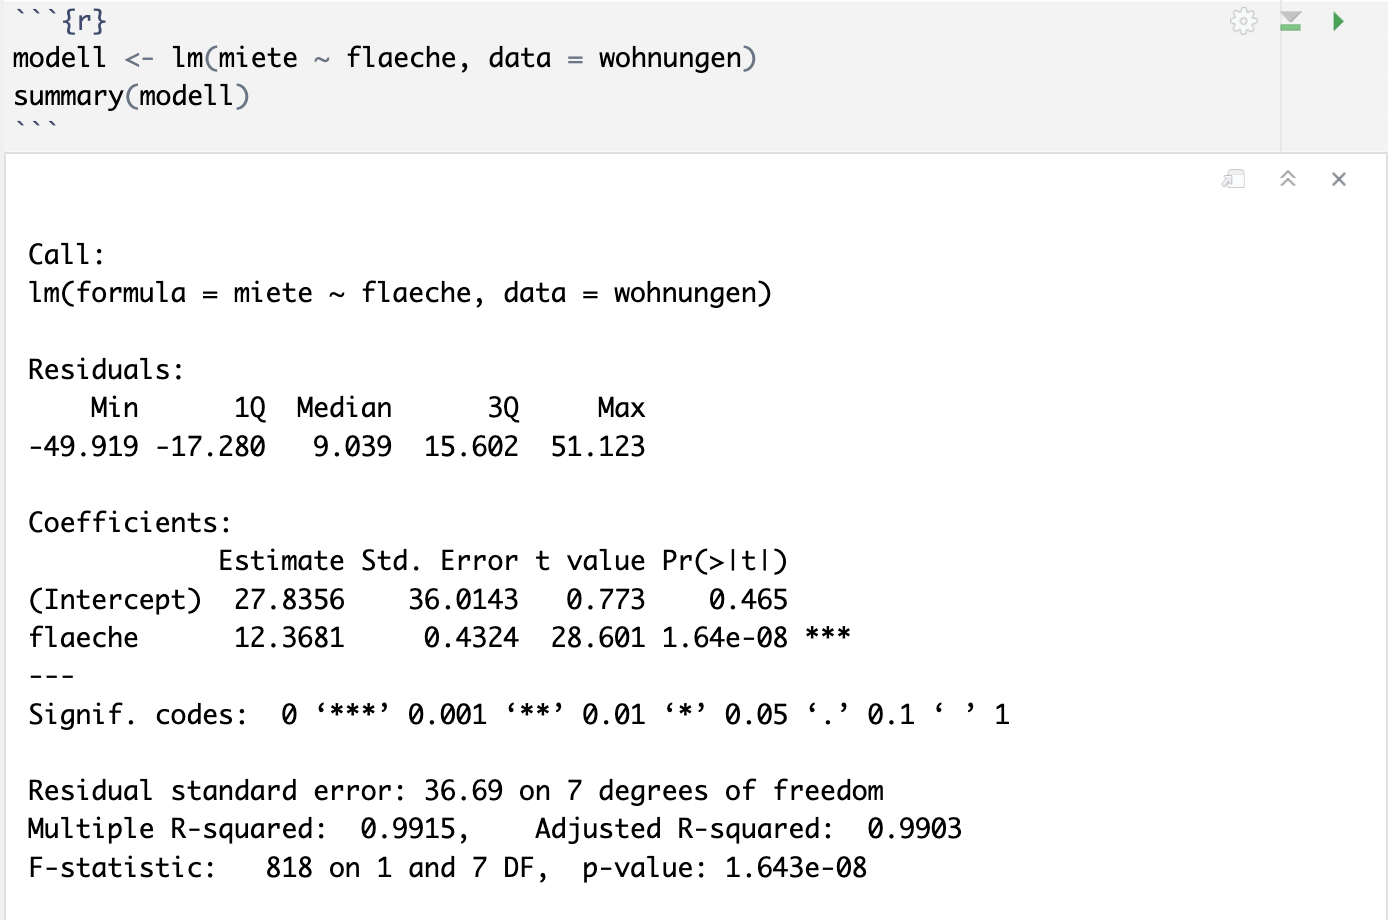
\includegraphics[keepaspectratio]{images/regression-ausgabe.png}}
\end{frame}

\begin{frame}{Modellgüte: Wie gut passt die Gerade?}
\protect\phantomsection\label{modellguxfcte-wie-gut-passt-die-gerade}
\begin{itemize}
\tightlist
\item
  R² = Anteil der erklärten Varianz
\item
  Beispiel: R² = 0.99 → 99\% der Mietunterschiede durch Fläche erklärbar
\item
  Residuenplot prüfen: Gibt es systematische Fehler?
\end{itemize}
\end{frame}

\begin{frame}{Residuenplot - Erwartung: Punkte gleichmäßig um die
Nulllinie verteilt}
\protect\phantomsection\label{residuenplot---erwartung-punkte-gleichmuxe4uxdfig-um-die-nulllinie-verteilt}
\pandocbounded{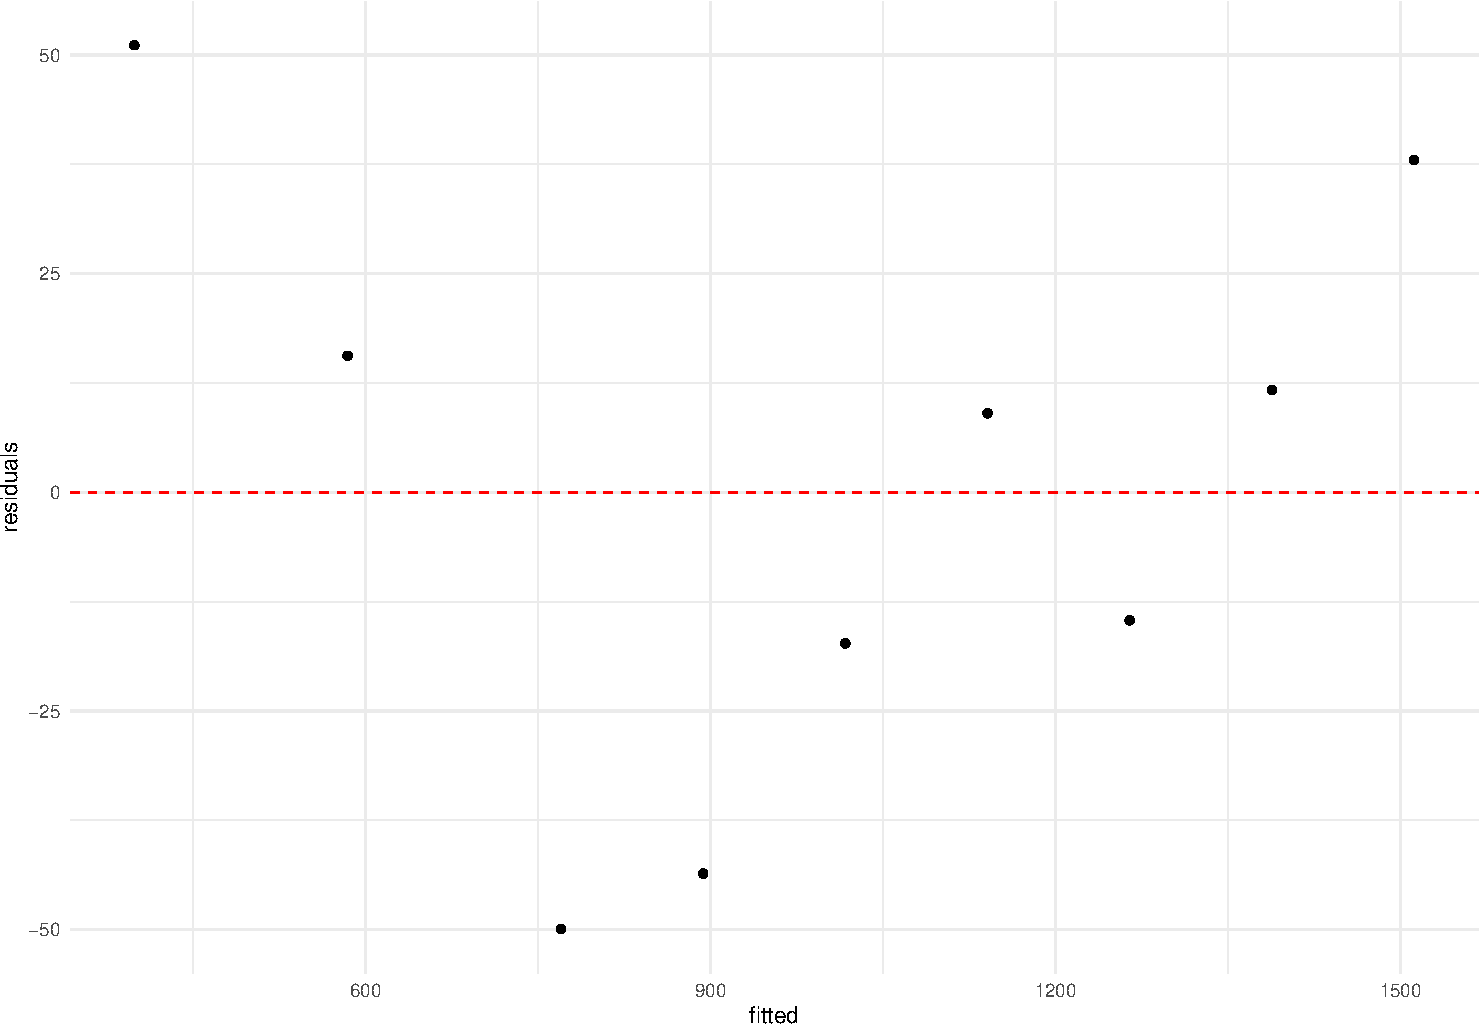
\includegraphics[keepaspectratio]{Statistik_Seminar_files/figure-beamer/unnamed-chunk-47-1.pdf}}
\end{frame}

\begin{frame}{Aber ist die Fläche wirklich die einzige unabhängige
Variable?}
\protect\phantomsection\label{aber-ist-die-fluxe4che-wirklich-die-einzige-unabhuxe4ngige-variable}
\end{frame}

\begin{frame}{Visualisierung der Daten}
\protect\phantomsection\label{visualisierung-der-daten}
\pandocbounded{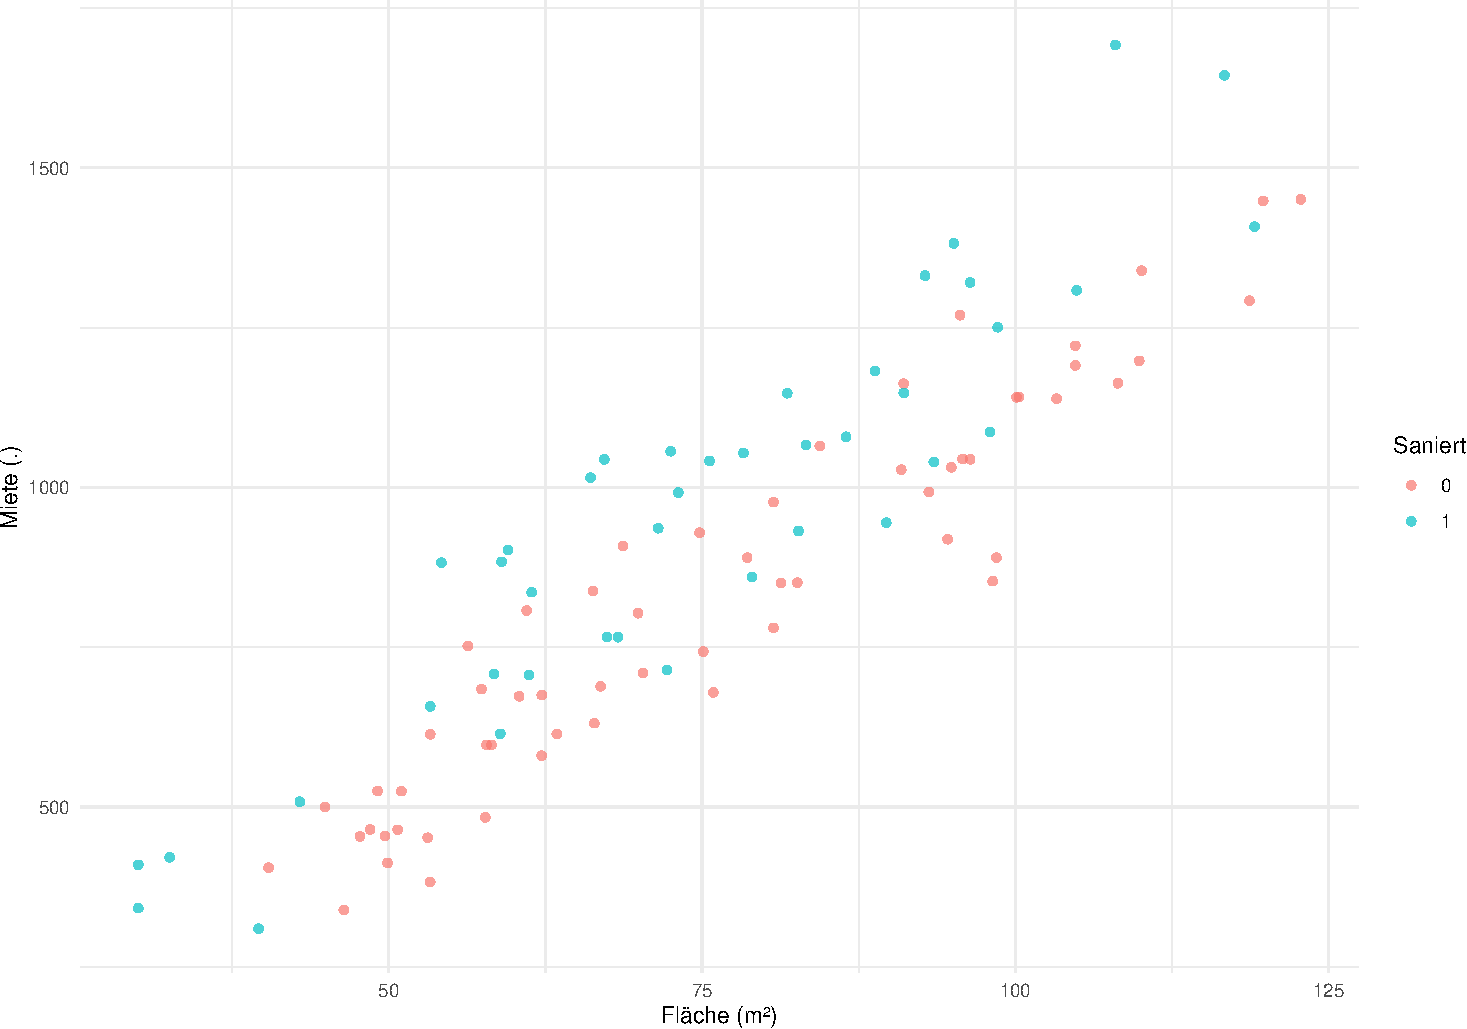
\includegraphics[keepaspectratio]{Statistik_Seminar_files/figure-beamer/unnamed-chunk-49-1.pdf}}
\end{frame}

\begin{frame}{Welchen Einfluss hat die Energieeffizienzklasse?}
\protect\phantomsection\label{welchen-einfluss-hat-die-energieeffizienzklasse}
\pandocbounded{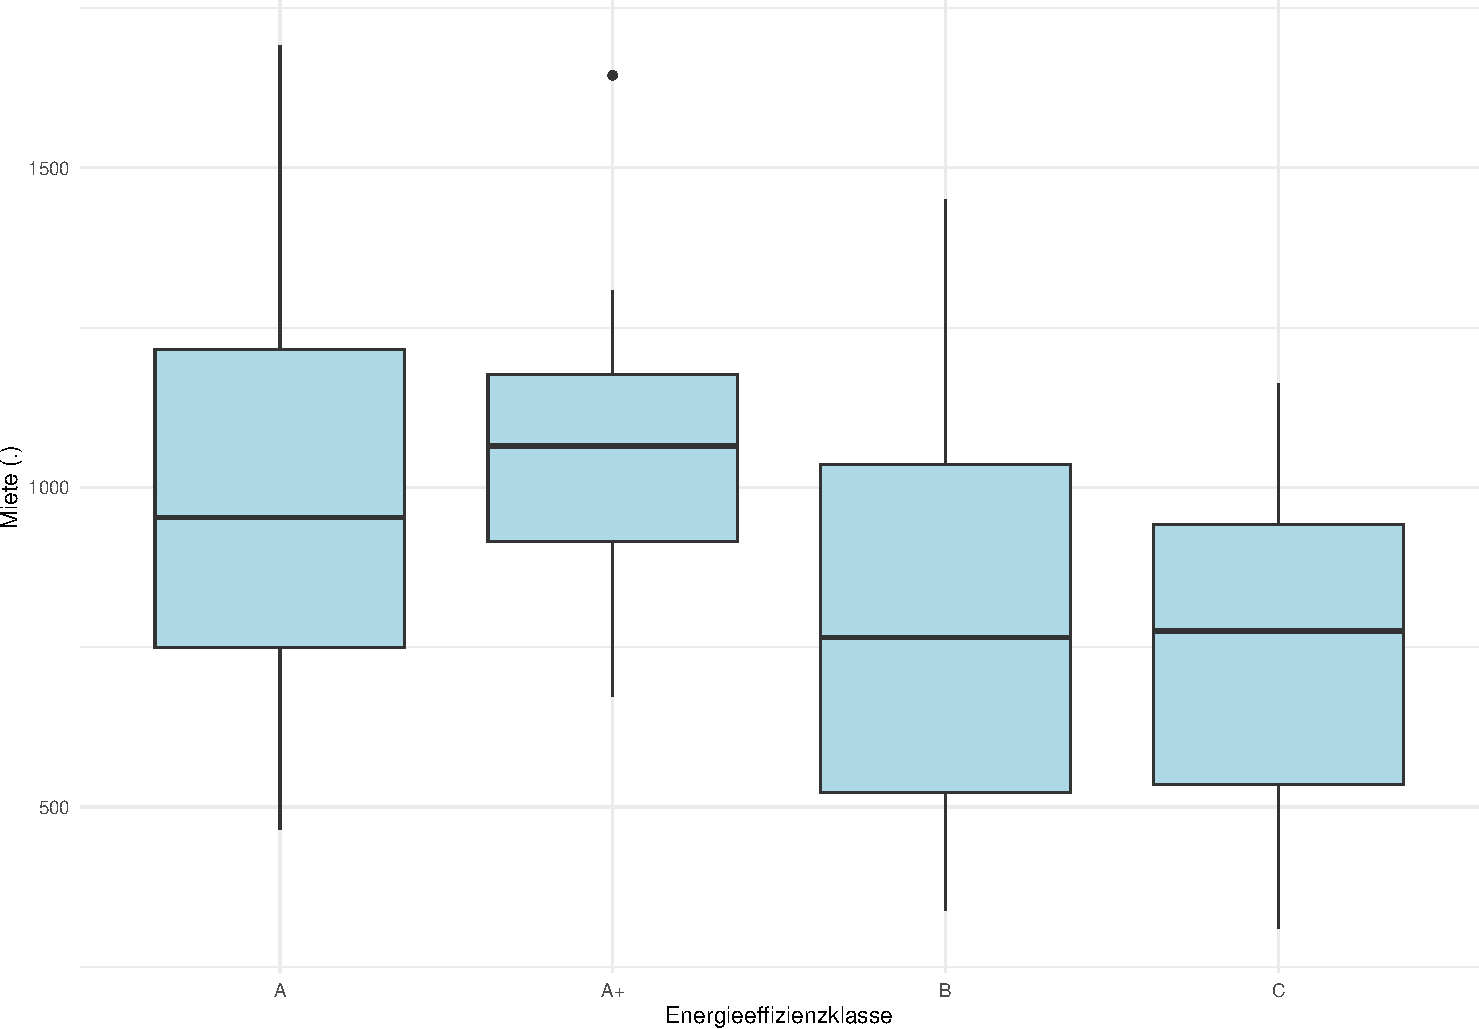
\includegraphics[keepaspectratio]{Statistik_Seminar_files/figure-beamer/unnamed-chunk-50-1.pdf}}
\end{frame}

\begin{frame}{Einfluss von Fläche und Energieeffizienz auf Miete}
\protect\phantomsection\label{einfluss-von-fluxe4che-und-energieeffizienz-auf-miete}
\pandocbounded{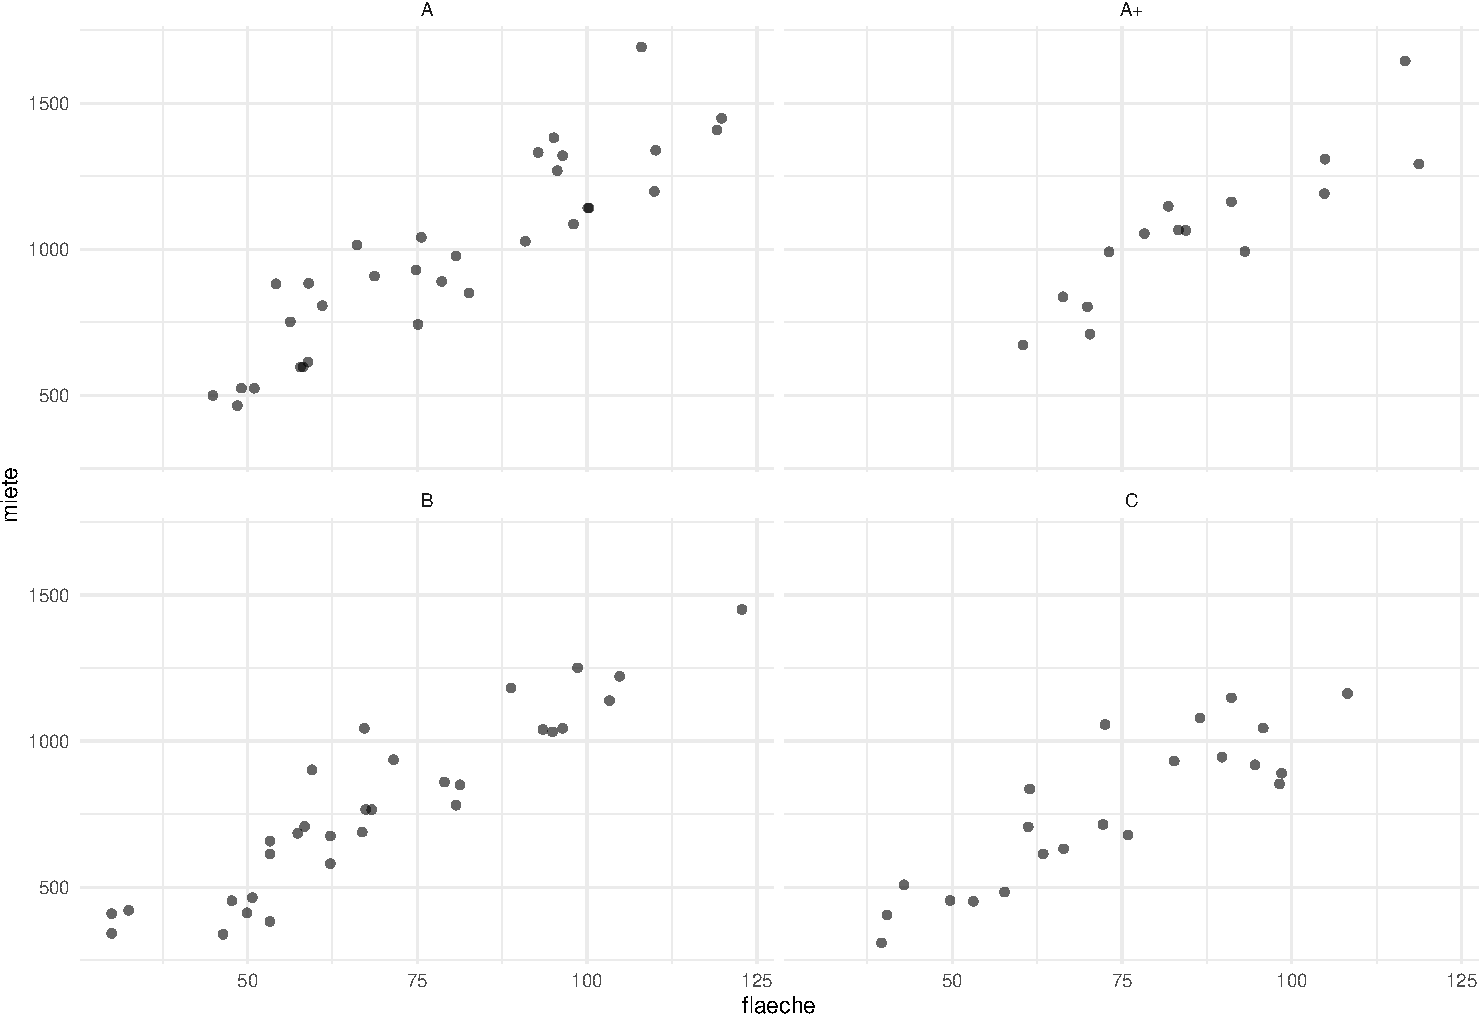
\includegraphics[keepaspectratio]{Statistik_Seminar_files/figure-beamer/unnamed-chunk-51-1.pdf}}
\end{frame}

\begin{frame}{Der Output}
\protect\phantomsection\label{der-output}
\end{frame}

\begin{frame}{\pandocbounded{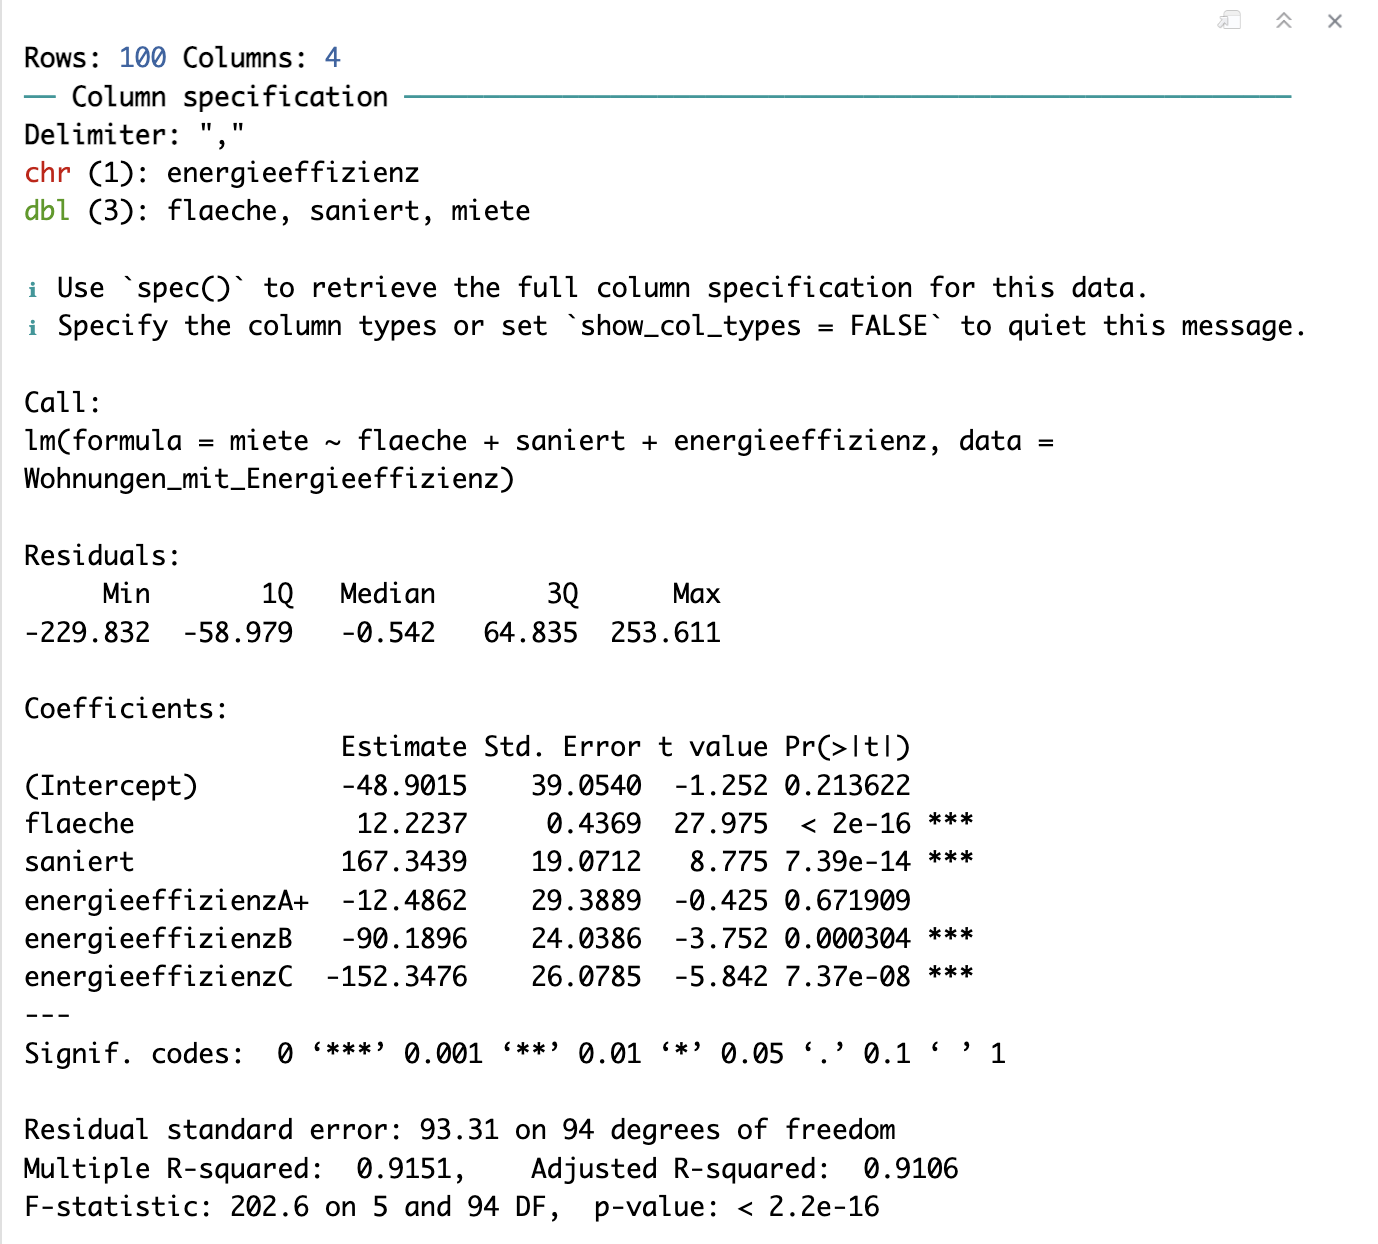
\includegraphics[keepaspectratio]{images/logit.png}}}
\protect\phantomsection\label{section}
\end{frame}

\begin{frame}{Wie funktioniert das mit der Linie mit mehr als zwei
Variablen?}
\protect\phantomsection\label{wie-funktioniert-das-mit-der-linie-mit-mehr-als-zwei-variablen}
\pandocbounded{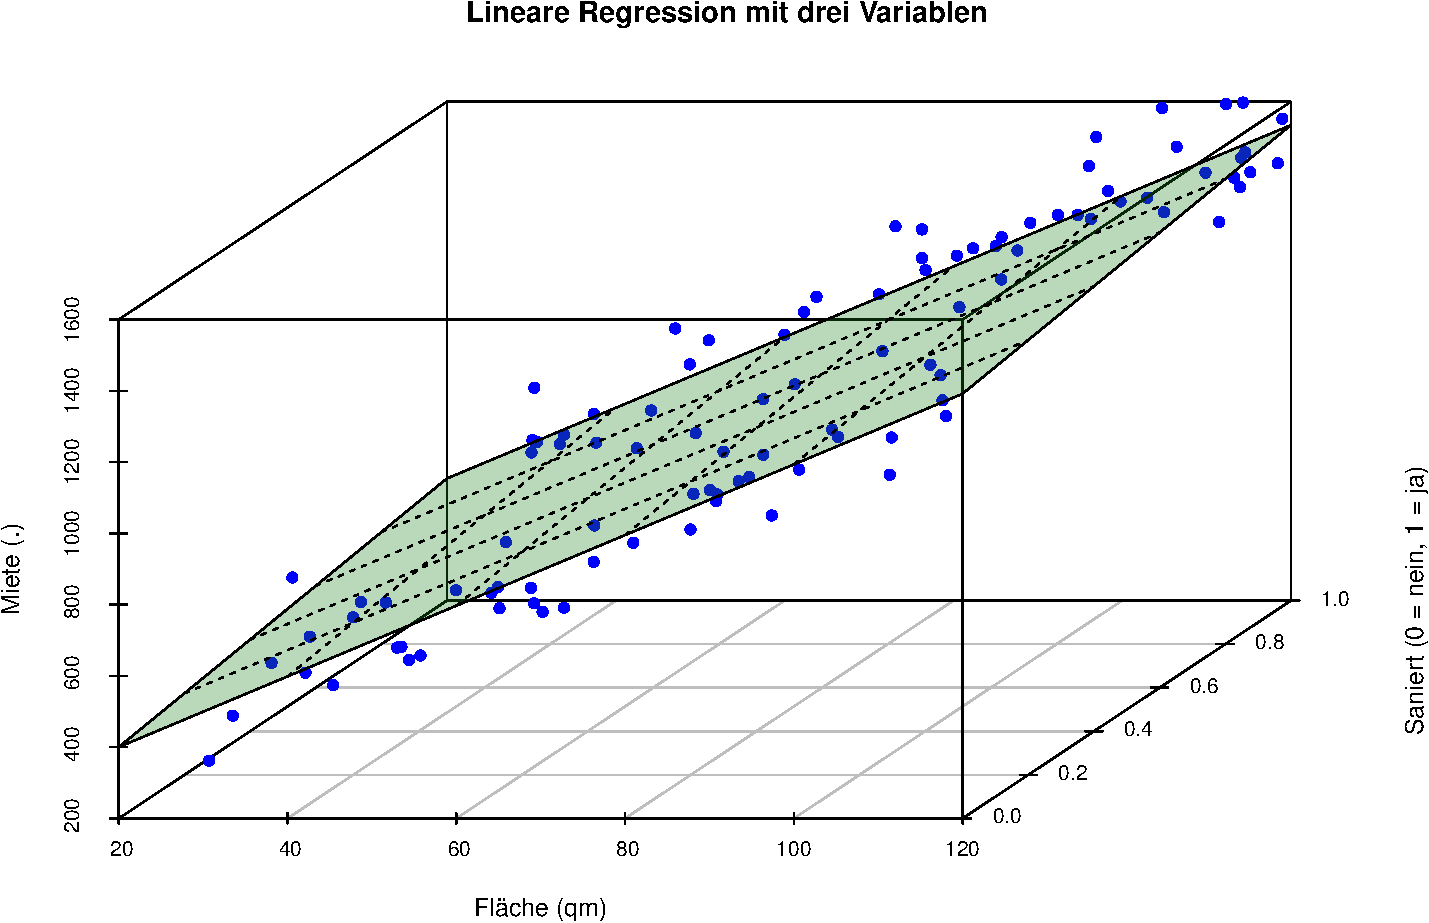
\includegraphics[keepaspectratio]{Statistik_Seminar_files/figure-beamer/unnamed-chunk-53-1.pdf}}
\end{frame}

\begin{frame}
\end{frame}

\section{Sitzung 13: Regression II -- Logistische
Regression}\label{sitzung-13-regression-ii-logistische-regression}

\begin{frame}{Lernziele dieser Sitzung}
\protect\phantomsection\label{lernziele-dieser-sitzung-9}
\begin{itemize}
\tightlist
\item
  Das Konzept der Log-Odds und der Logit-Transformation erklären
\item
  Eine logistische Regression in R schätzen und interpretieren
\item
  Odds Ratios berechnen und kommunizieren
\item
  Die S-Kurve und ihre Bedeutung verstehen
\item
  Lineare und logistische Regression gegenüberstellen
\end{itemize}
\end{frame}

\begin{frame}{Jetzt wird's binär: Logistische Regression}
\protect\phantomsection\label{jetzt-wirds-binuxe4r-logistische-regression}
Frage: Stirbt ein Titanic-Passagier oder nicht? Und welche Faktoren
führen dazu?
\end{frame}

\begin{frame}{Was sind Log-Odds?}
\protect\phantomsection\label{was-sind-log-odds}
In der logistischen Regression wird \textbf{nicht direkt die
Wahrscheinlichkeit} geschätzt, sondern:

\[\log\left(\frac{p}{1 - p}\right)\]

Das ist der sogenannte \textbf{Logit} -- also der \textbf{logarithmierte
Quotient der Wahrscheinlichkeit und ihrer Gegenwahrscheinlichkeit}.

--
\end{frame}

\begin{frame}{Was ist ein Logarithmus?}
\protect\phantomsection\label{was-ist-ein-logarithmus}
\begin{itemize}
\tightlist
\item
  Der \textbf{Logarithmus} ist die Umkehrung der Potenzierung:
\end{itemize}

\[  \log_{10}(1000) = 3 \quad \text{denn } 10^3 = 1000\]
\end{frame}

\begin{frame}
\begin{block}{Merksatz:}
\protect\phantomsection\label{merksatz}
\begin{quote}
Der Logarithmus transformiert Werte in ein \textbf{lineares Maß}, das
für Regressionsmodelle besser handhabbar ist -- auch wenn die
ursprünglichen Wahrscheinlichkeiten zwischen 0 und 1 liegen.
\end{quote}
\end{block}
\end{frame}

\begin{frame}{Warum Log-Odds?}
\protect\phantomsection\label{warum-log-odds}
\begin{itemize}
\item
  Wahrscheinlichkeiten liegen \textbf{zwischen 0 und 1}
\item
  Log-Odds hingegen können \textbf{alle Werte zwischen --∞ und +∞}
  annehmen
\item
  So kann ein \textbf{lineares Modell} verwendet werden:

  \[\log\left(\frac{p}{1 - p}\right) = \beta_0 + \beta_1 x_1 + \dots + \beta_k x_k \]
\end{itemize}
\end{frame}

\begin{frame}{Beispiel:}
\protect\phantomsection\label{beispiel}
{\def\LTcaptype{none} % do not increment counter
\begin{longtable}[]{@{}
  >{\raggedright\arraybackslash}p{(\linewidth - 8\tabcolsep) * \real{0.2000}}
  >{\raggedright\arraybackslash}p{(\linewidth - 8\tabcolsep) * \real{0.2000}}
  >{\raggedright\arraybackslash}p{(\linewidth - 8\tabcolsep) * \real{0.2000}}
  >{\raggedright\arraybackslash}p{(\linewidth - 8\tabcolsep) * \real{0.2000}}
  >{\raggedright\arraybackslash}p{(\linewidth - 8\tabcolsep) * \real{0.2000}}@{}}
\toprule\noalign{}
\begin{minipage}[b]{\linewidth}\raggedright
Wahrscheinlichkeit (p)
\end{minipage} & \begin{minipage}[b]{\linewidth}\raggedright
Gegenwahrscheinlichkeit (1 - p)
\end{minipage} & \begin{minipage}[b]{\linewidth}\raggedright
Verhältnis (Odds) (p : (1 - p))
\end{minipage} & \begin{minipage}[b]{\linewidth}\raggedright
Odds (als Zahl) (\frac{p}{1 - p})
\end{minipage} & \begin{minipage}[b]{\linewidth}\raggedright
Log-Odds (\log\left(\frac{p}{1 - p}\right))
\end{minipage} \\
\midrule\noalign{}
\endhead
0.10 & 0.90 & 1 : 9 & 0.111 & --2.20 \\
0.50 & 0.50 & 1 : 1 & 1.000 & 0.00 \\
0.90 & 0.10 & 9 : 1 & 9.000 & 2.20 \\
\bottomrule\noalign{}
\end{longtable}
}
\end{frame}

\begin{frame}{Merksatz:}
\protect\phantomsection\label{merksatz-1}
\textbf{Log-Odds} sind eine \textbf{Umformung der Wahrscheinlichkeit}
und erlauben \textbf{lineare Modellierung} auf einer unbeschränkten
Skala.
\end{frame}

\begin{frame}[fragile]{Zunächst müssen wir die Daten vorbereiten}
\protect\phantomsection\label{zunuxe4chst-muxfcssen-wir-die-daten-vorbereiten}
\begin{Shaded}
\begin{Highlighting}[]
\NormalTok{titanic }\OtherTok{\textless{}{-}}\NormalTok{ titanic\_train }\SpecialCharTok{\%\textgreater{}\%}
  \FunctionTok{select}\NormalTok{(Survived, Pclass, Sex, Age) }\SpecialCharTok{\%\textgreater{}\%}
  \FunctionTok{filter}\NormalTok{(}\SpecialCharTok{!}\FunctionTok{is.na}\NormalTok{(Age)) }\SpecialCharTok{\%\textgreater{}\%}
  \FunctionTok{mutate}\NormalTok{(}
    \AttributeTok{Survived =} \FunctionTok{factor}\NormalTok{(Survived, }\AttributeTok{labels =} \FunctionTok{c}\NormalTok{(}\StringTok{"Gestorben"}\NormalTok{, }\StringTok{"Überlebt"}\NormalTok{)),}
    \AttributeTok{Sex =} \FunctionTok{factor}\NormalTok{(Sex),}
    \AttributeTok{Pclass =} \FunctionTok{factor}\NormalTok{(Pclass)}
\NormalTok{  )}
\end{Highlighting}
\end{Shaded}
\end{frame}

\begin{frame}{Der Output}
\protect\phantomsection\label{der-output-1}
\pandocbounded{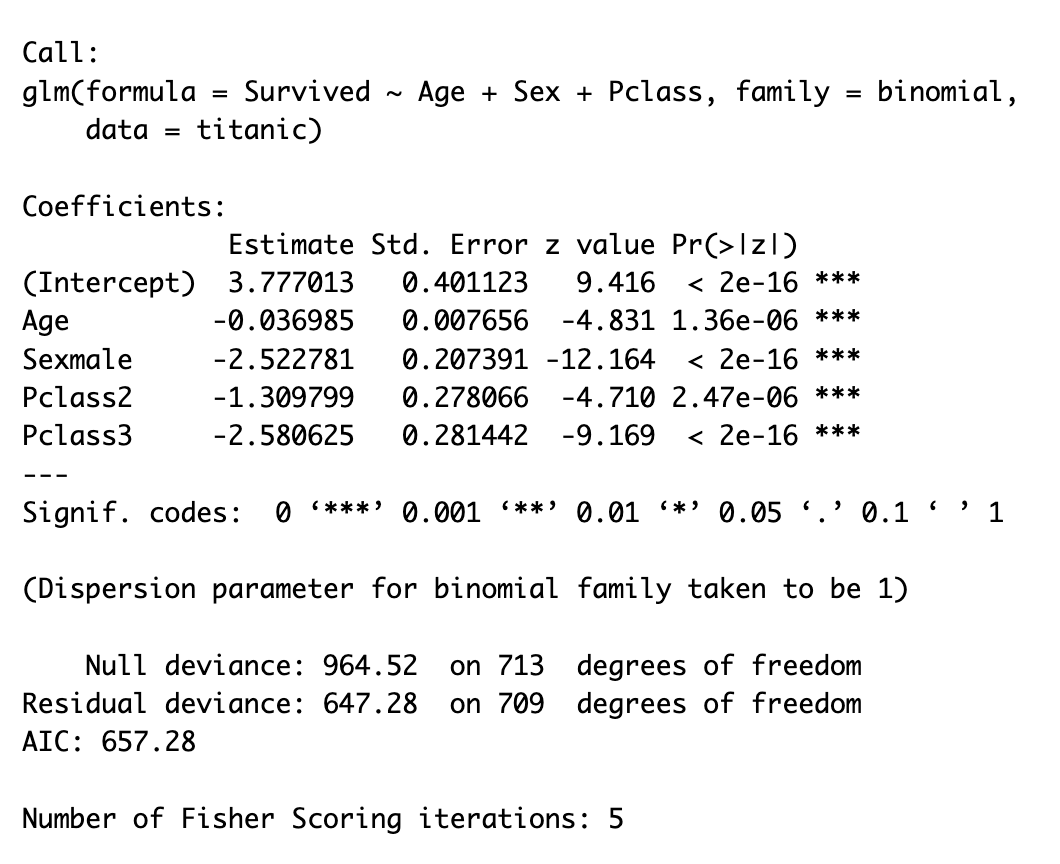
\includegraphics[keepaspectratio]{images/titanic-logit.png}}
\end{frame}

\begin{frame}{Ausgabe der LogOdds}
\protect\phantomsection\label{ausgabe-der-logodds}
\pandocbounded{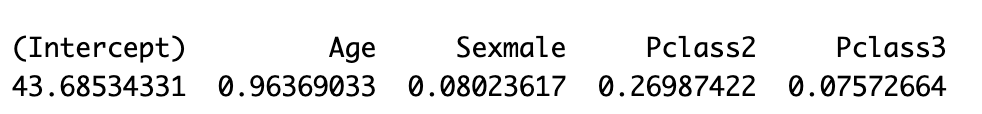
\includegraphics[keepaspectratio]{images/logodds.png}}
\end{frame}

\begin{frame}{S-Kurve}
\protect\phantomsection\label{s-kurve}
\pandocbounded{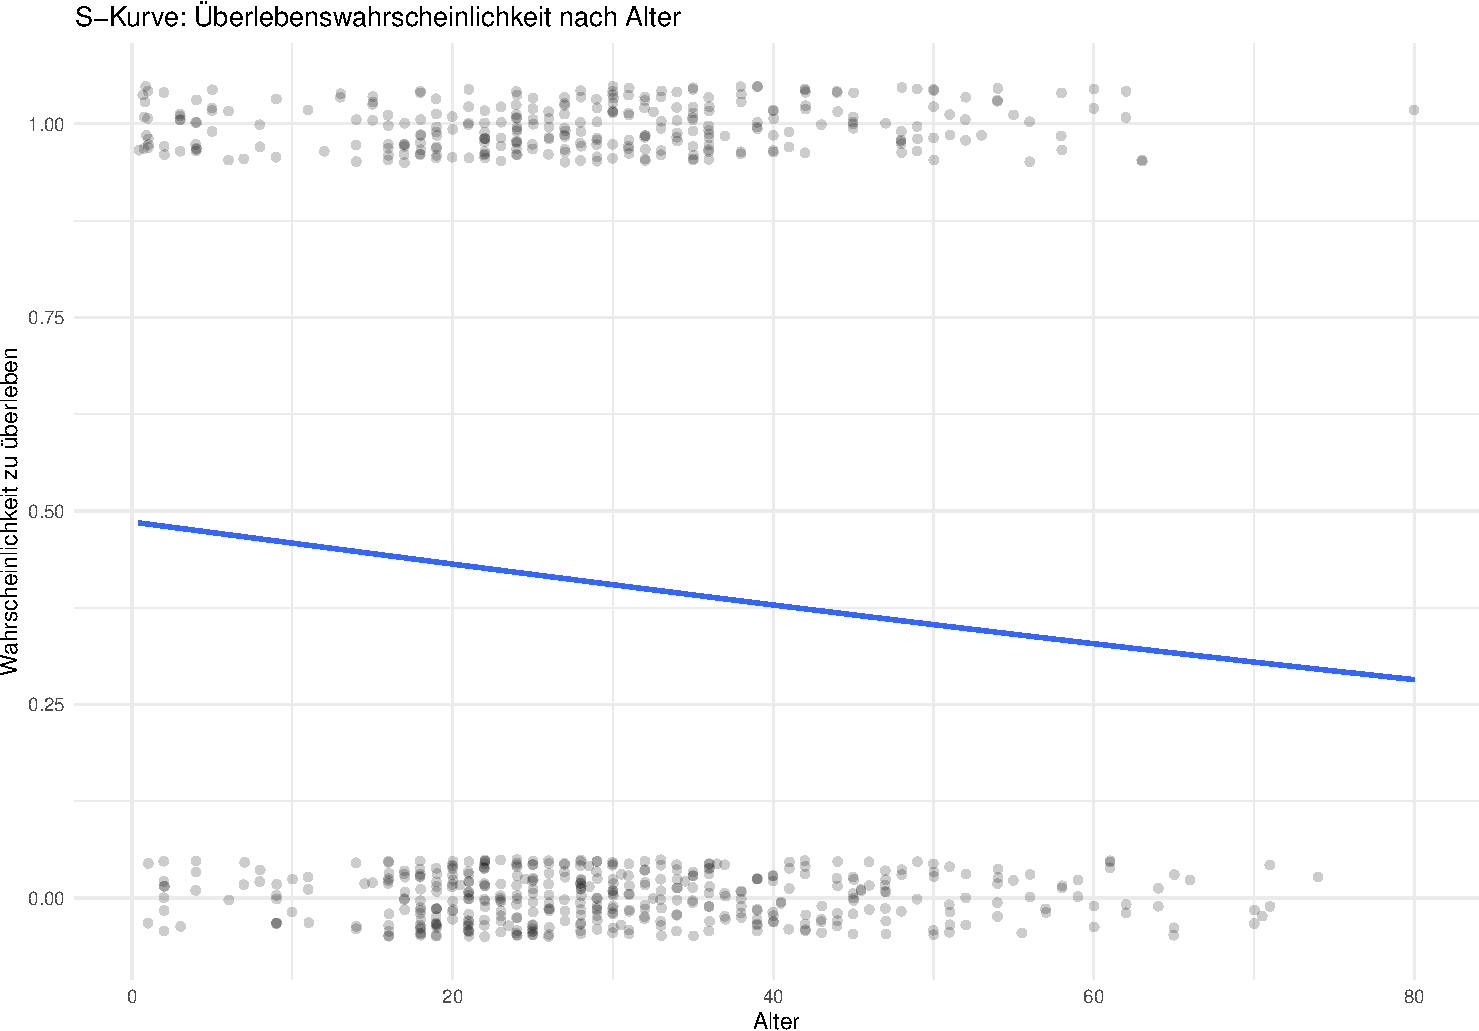
\includegraphics[keepaspectratio]{Statistik_Seminar_files/figure-beamer/unnamed-chunk-58-1.pdf}}
\end{frame}

\begin{frame}{S-Kurve II}
\protect\phantomsection\label{s-kurve-ii}
\pandocbounded{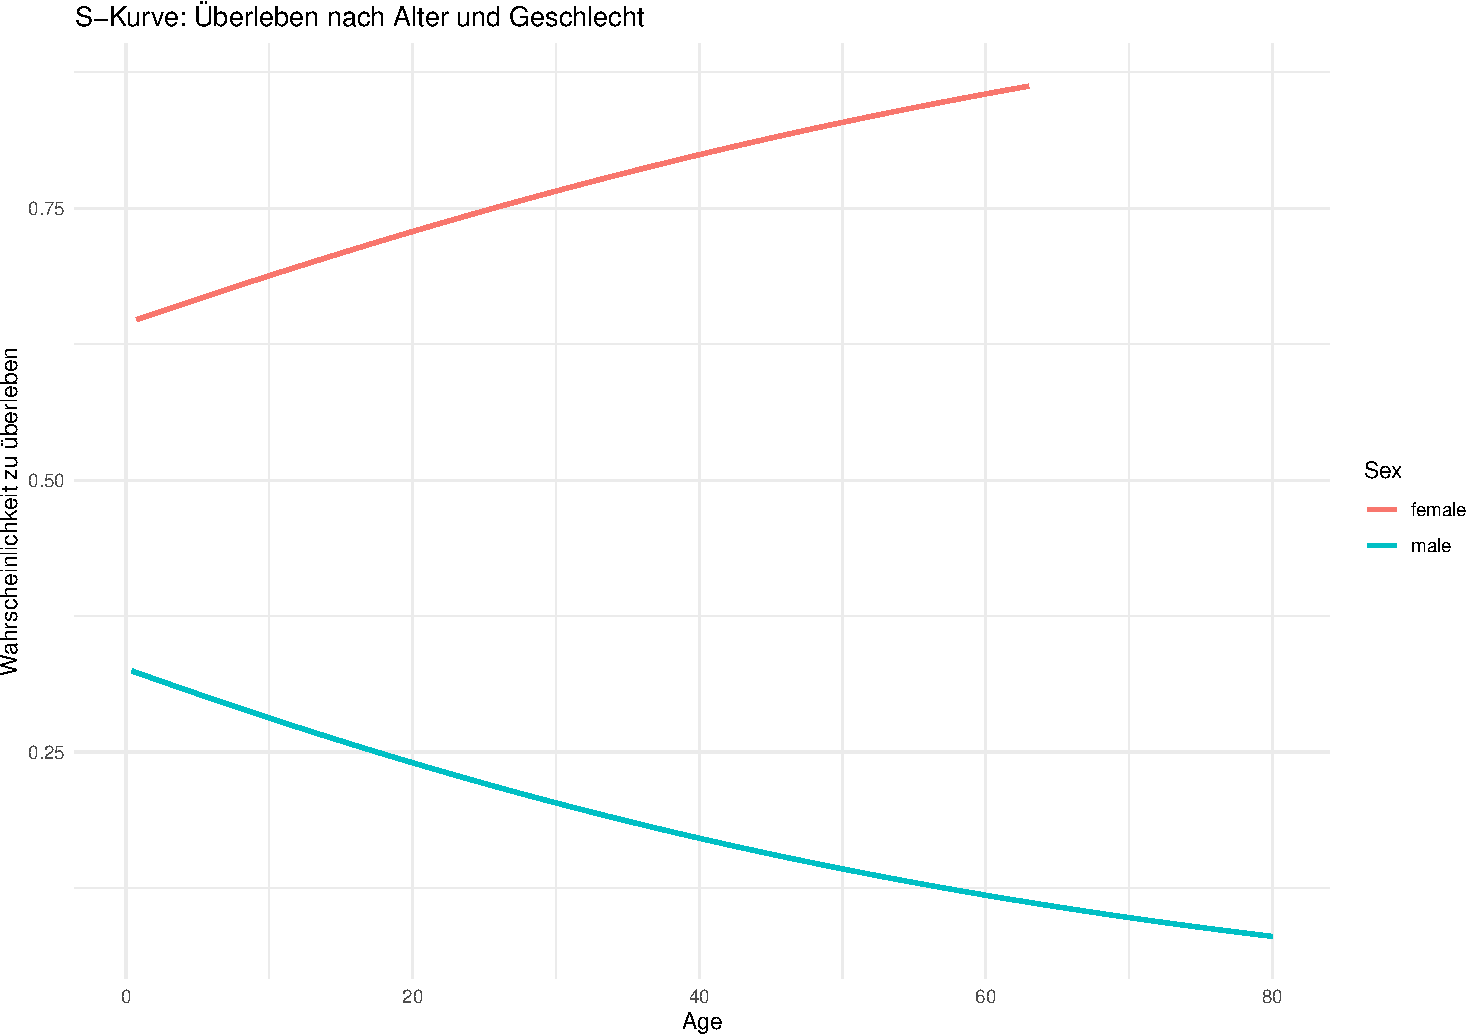
\includegraphics[keepaspectratio]{Statistik_Seminar_files/figure-beamer/unnamed-chunk-59-1.pdf}}
\end{frame}

\begin{frame}{Vergleich: Lineare vs.~Logistische Regression}
\protect\phantomsection\label{vergleich-lineare-vs.-logistische-regression}
{\def\LTcaptype{none} % do not increment counter
\begin{longtable}[]{@{}
  >{\raggedright\arraybackslash}p{(\linewidth - 4\tabcolsep) * \real{0.2254}}
  >{\raggedright\arraybackslash}p{(\linewidth - 4\tabcolsep) * \real{0.3239}}
  >{\raggedright\arraybackslash}p{(\linewidth - 4\tabcolsep) * \real{0.4507}}@{}}
\toprule\noalign{}
\begin{minipage}[b]{\linewidth}\raggedright
Aspekt
\end{minipage} & \begin{minipage}[b]{\linewidth}\raggedright
Lineare Regression
\end{minipage} & \begin{minipage}[b]{\linewidth}\raggedright
Logistische Regression
\end{minipage} \\
\midrule\noalign{}
\endhead
Zielvariable Y & metrisch (z.B. Preis) & binär (z.B. gestorben
ja/nein) \\
Ergebnis & Gerade & S-Kurve \\
Vorhersage & Reeller Zahlenwert & Wahrscheinlichkeit (0--1) \\
Residuen & Differenz & Abweichung in Log-Odds \\
Interpretation & Effekt pro X & Odds Ratio \\
\bottomrule\noalign{}
\end{longtable}
}
\end{frame}

\begin{frame}{Unterschied Korrelation zu Regression}
\protect\phantomsection\label{unterschied-korrelation-zu-regression}
\begin{itemize}
\item
  \textbf{Korrelation} beschreibt \textbf{Stärke und Richtung} eines
  \textbf{linearen Zusammenhangs} zwischen zwei numerischen Variablen,
  ohne Einflussrichtung oder Kausalität anzunehmen.
\item
  \textbf{Lineare Regression} modelliert eine \textbf{gerichtete lineare
  Beziehung} zwischen einer abhängigen Variable und einer oder mehreren
  unabhängigen Variablen mit der \textbf{Stärke des Einflusses}.
\end{itemize}
\end{frame}

\begin{frame}{Unterschied Korrelation zu Regression}
\protect\phantomsection\label{unterschied-korrelation-zu-regression-1}
\begin{itemize}
\tightlist
\item
  \textbf{Logistische Regression} schätzt die
  \textbf{Wahrscheinlichkeit} für das Eintreten eines \textbf{binären
  Ereignisses} auf Basis einer oder mehrerer Einflussvariablen und
  liefert eine \textbf{gerichtete Interpretation}.
\end{itemize}
\end{frame}

\begin{frame}
\end{frame}

\section{Sitzung 11: ANOVA}\label{sitzung-11-anova}

\begin{frame}{Lernziele dieser Sitzung}
\protect\phantomsection\label{lernziele-dieser-sitzung-10}
\begin{itemize}
\tightlist
\item
  ANOVA als Erweiterung des t-Tests auf mehr als zwei Gruppen einordnen
\item
  Varianzzerlegung und F-Statistik verstehen
\item
  Eine einfaktorielle ANOVA in R durchführen
\item
  Post-hoc-Tests (Tukey HSD) korrekt einsetzen
\item
  Den passenden Test für den eigenen Datensatz wählen
\end{itemize}
\end{frame}

\begin{frame}{Was ist ANOVA?}
\protect\phantomsection\label{was-ist-anova}
\begin{itemize}
\tightlist
\item
  ANOVA = Analysis of Variance = Varianzanalyse
\item
  Prüft, ob sich Gruppenmittelwerte signifikant unterscheiden
\item
  Erweiterung des t-Tests auf mehr als zwei Gruppen
\item
  Beispiel: Unterschiedet sich die durchschnittliche Miete in
  verschiedenen Stadtteilen?
\end{itemize}
\end{frame}

\begin{frame}{Wann nutzt man ANOVA?}
\protect\phantomsection\label{wann-nutzt-man-anova}
\begin{itemize}
\tightlist
\item
  Abhängige Variable metrisch (z.B. Einkommen, Preis, Größe)
\item
  Unabhängige Variable kategorial (z.B. Stadtteil, Behandlungsmethode)
\item
  Mehr als zwei Gruppen zu vergleichen
\item
  Ziel: Test auf Mittelwertsunterschiede
\end{itemize}
\end{frame}

\begin{frame}{Grundidee der ANOVA}
\protect\phantomsection\label{grundidee-der-anova}
\begin{itemize}
\tightlist
\item
  Zerlegung der Gesamtvarianz:

  \begin{itemize}
  \tightlist
  \item
    \textbf{Zwischen-Gruppen-Varianz}: Unterschiede zwischen den
    Gruppenmitteln
  \item
    \textbf{Innerhalb-Gruppen-Varianz}: Streuung innerhalb der Gruppen
  \end{itemize}
\item
  Wenn die Zwischen-Gruppen-Varianz groß im Vergleich zur
  Innerhalb-Gruppen-Varianz ist → Hinweis auf echte Unterschiede
\end{itemize}
\end{frame}

\begin{frame}{Beispiel: Schmerzmittel-Wirkung}
\protect\phantomsection\label{beispiel-schmerzmittel-wirkung}
\begin{itemize}
\tightlist
\item
  Fragestellung: Unterscheidet sich die durchschnittliche
  Schmerzreduktion bei drei Medikamenten?
\item
  Gruppen:

  \begin{itemize}
  \tightlist
  \item
    Medikament A
  \item
    Medikament B
  \item
    Placebo
  \end{itemize}
\item
  Abhängige Variable: Schmerzscore nach 30 Minuten (Skala 0-10)
\item
  ANOVA prüft, ob es signifikante Unterschiede gibt
\end{itemize}
\end{frame}

\begin{frame}{Beispiel: Werbewirkung testen}
\protect\phantomsection\label{beispiel-werbewirkung-testen}
\begin{itemize}
\tightlist
\item
  Fragestellung: Führt die Art der Werbeanzeige zu unterschiedlichen
  Kaufabsichten?
\item
  Gruppen:

  \begin{itemize}
  \tightlist
  \item
    Emotionaler Spot
  \item
    Sachlicher Spot
  \item
    Keine Werbung (Kontrollgruppe)
  \end{itemize}
\item
  Abhängige Variable: Kaufwahrscheinlichkeit (Skala 0-100\%)
\item
  ANOVA zeigt, ob mindestens eine Gruppe signifikant abweicht
\end{itemize}
\end{frame}

\begin{frame}{Beispiel: Einfluss von Dünger}
\protect\phantomsection\label{beispiel-einfluss-von-duxfcnger}
\begin{itemize}
\tightlist
\item
  Fragestellung: Hat die Düngersorte Einfluss auf das Pflanzenwachstum?
\item
  Gruppen:

  \begin{itemize}
  \tightlist
  \item
    Dünger X
  \item
    Dünger Y
  \item
    Kein Dünger
  \end{itemize}
\item
  Abhängige Variable: Pflanzenhöhe nach 6 Wochen (in cm)
\item
  ANOVA prüft auf Unterschiede der mittleren Pflanzenhöhe
\end{itemize}
\end{frame}

\begin{frame}{Hypothesen der ANOVA}
\protect\phantomsection\label{hypothesen-der-anova}
\begin{itemize}
\tightlist
\item
  \textbf{Nullhypothese (H₀)}: Alle Gruppenmittelwerte sind gleich
\item
  \textbf{Alternativhypothese (H₁)}: Mindestens zwei Gruppen
  unterscheiden sich im Mittelwert
\end{itemize}
\end{frame}

\begin{frame}[fragile]{Beispiel in R}
\protect\phantomsection\label{beispiel-in-r}
\begin{verbatim}
            Df Sum Sq Mean Sq F value   Pr(>F)    
gruppe       2  32.71   16.35   19.23 4.15e-07 ***
Residuals   57  48.48    0.85                     
---
Signif. codes:  0 '***' 0.001 '**' 0.01 '*' 0.05 '.' 0.1 ' ' 1
\end{verbatim}
\end{frame}

\begin{frame}{Interpretation der Ausgabe}
\protect\phantomsection\label{interpretation-der-ausgabe}
\begin{itemize}
\tightlist
\item
  \textbf{F-Wert}: Teststatistik, je größer desto mehr Hinweis auf
  Unterschied
\item
  \textbf{p-Wert}: Ist p \textless{} 0.05 → Ablehnung der Nullhypothese
\item
  Achtung: ANOVA zeigt nur, \emph{dass} ein Unterschied vorliegt, nicht
  \emph{wo} genau
\end{itemize}
\end{frame}

\begin{frame}{Post-hoc-Tests}
\protect\phantomsection\label{post-hoc-tests}
\begin{itemize}
\tightlist
\item
  Notwendig, wenn ANOVA signifikant ist
\item
  Beispiele:

  \begin{itemize}
  \tightlist
  \item
    Tukey HSD-Test (bei Varianzhomogenität)
  \item
    Games-Howell-Test (bei ungleichen Varianzen)
  \end{itemize}
\item
  Zeigt, zwischen welchen Gruppen die Unterschiede liegen
\end{itemize}
\end{frame}

\begin{frame}[fragile]{Der Levene-Test}
\protect\phantomsection\label{der-levene-test}
\begin{verbatim}
Levene's Test for Homogeneity of Variance (center = median)
      Df F value Pr(>F)
group  2  0.0338 0.9668
      57               
\end{verbatim}
\end{frame}

\begin{frame}{Tukey HSD-Test}
\protect\phantomsection\label{tukey-hsd-test}
\pandocbounded{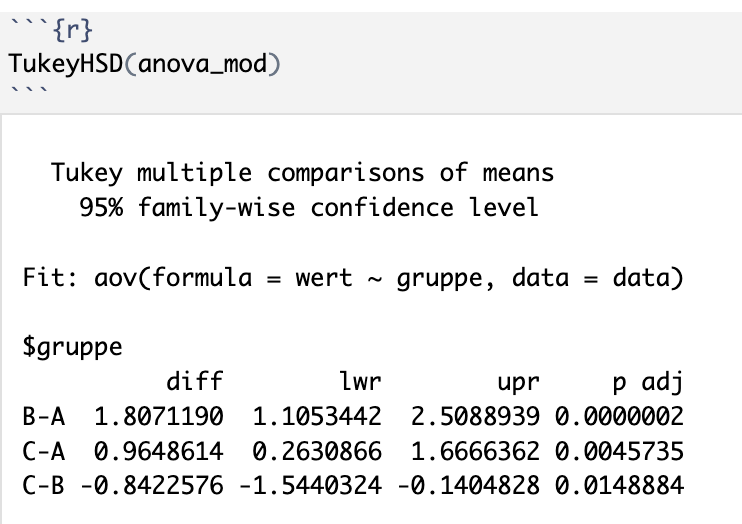
\includegraphics[keepaspectratio]{images/anova.png}}
\end{frame}

\begin{frame}{Ergebnisse visualisieren}
\protect\phantomsection\label{ergebnisse-visualisieren}
\pandocbounded{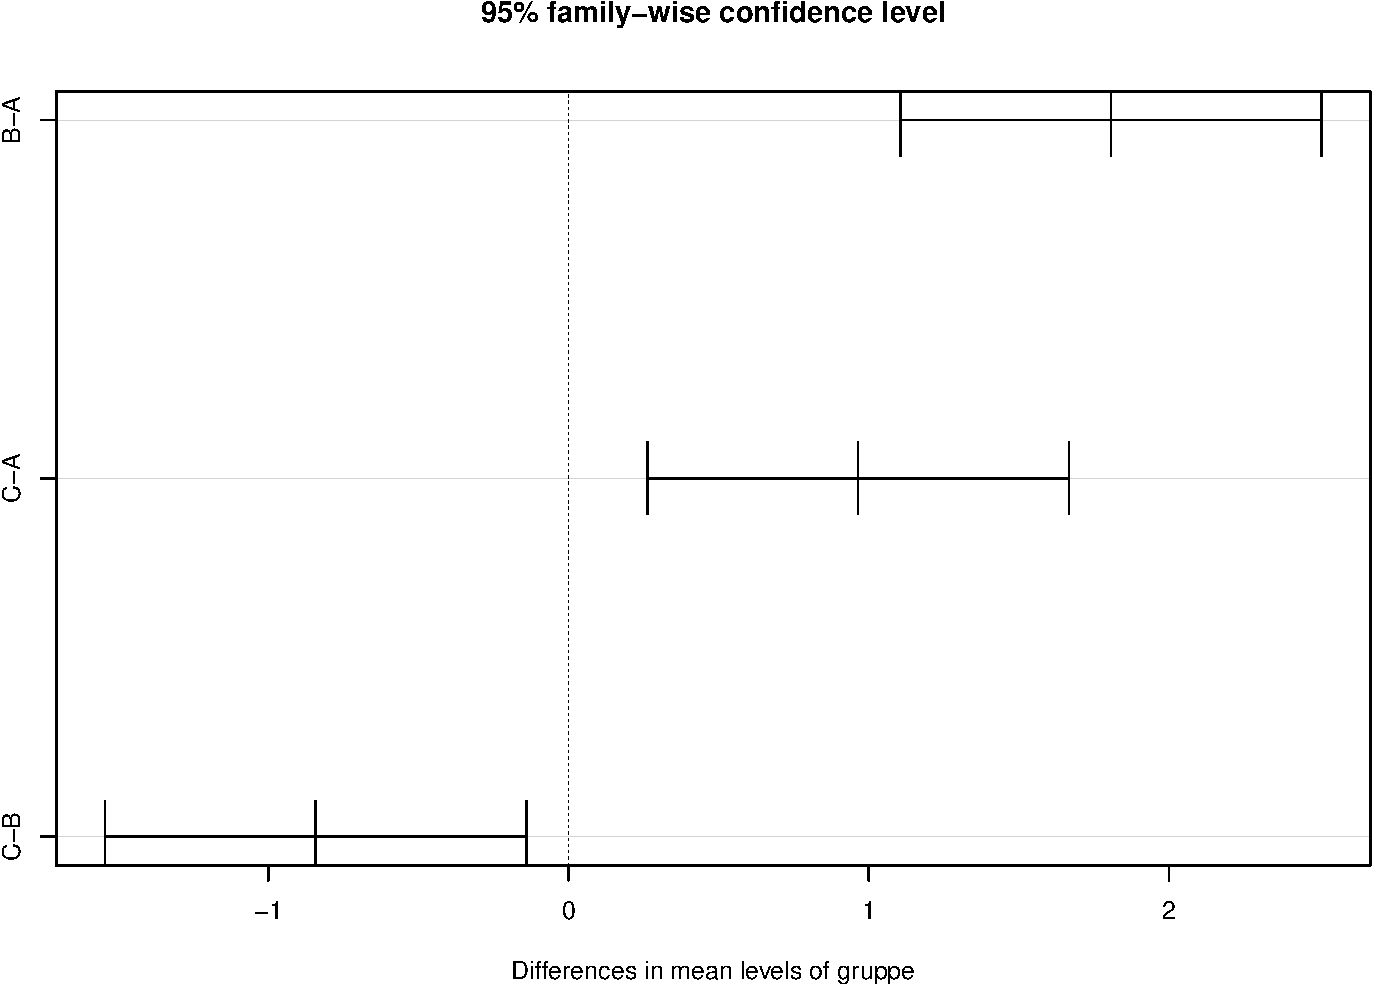
\includegraphics[keepaspectratio]{Statistik_Seminar_files/figure-beamer/unnamed-chunk-64-1.pdf}}
\end{frame}

\begin{frame}{Voraussetzungen der ANOVA}
\protect\phantomsection\label{voraussetzungen-der-anova}
\begin{itemize}
\tightlist
\item
  Unabhängigkeit der Beobachtungen
\item
  Normalverteilung innerhalb der Gruppen
\item
  Varianzhomogenität (Levene-Test prüfen)
\item
  Robustheit bei kleinen Abweichungen gegeben
\end{itemize}
\end{frame}

\begin{frame}[fragile]{Was tun, wenn Voraussetzungen verletzt sind?
Nicht-parametrische Tests}
\protect\phantomsection\label{was-tun-wenn-voraussetzungen-verletzt-sind-nicht-parametrische-tests}
{\def\LTcaptype{none} % do not increment counter
\begin{longtable}[]{@{}
  >{\raggedright\arraybackslash}p{(\linewidth - 4\tabcolsep) * \real{0.3333}}
  >{\raggedright\arraybackslash}p{(\linewidth - 4\tabcolsep) * \real{0.3333}}
  >{\raggedright\arraybackslash}p{(\linewidth - 4\tabcolsep) * \real{0.3333}}@{}}
\toprule\noalign{}
\begin{minipage}[b]{\linewidth}\raggedright
Parametrisch
\end{minipage} & \begin{minipage}[b]{\linewidth}\raggedright
Nicht-parametrische Alternative
\end{minipage} & \begin{minipage}[b]{\linewidth}\raggedright
Wann?
\end{minipage} \\
\midrule\noalign{}
\endhead
t-Test (unabh.) & Mann-Whitney-U-Test & Keine Normalverteilung, kleine
n \\
t-Test (gepaart) & Wilcoxon-Vorzeichen-Rang-Test & Verbundene
Stichproben, ordinal \\
ANOVA & Kruskal-Wallis-Test & Mehr als 2 Gruppen, keine
Normalverteilung \\
\bottomrule\noalign{}
\end{longtable}
}

\begin{Shaded}
\begin{Highlighting}[]
\CommentTok{\# Beispiele}
\FunctionTok{wilcox.test}\NormalTok{(x, y)                          }\CommentTok{\# Mann{-}Whitney{-}U}
\FunctionTok{wilcox.test}\NormalTok{(before, after, }\AttributeTok{paired =} \ConstantTok{TRUE}\NormalTok{)  }\CommentTok{\# Wilcoxon gepaart}
\FunctionTok{kruskal.test}\NormalTok{(wert }\SpecialCharTok{\textasciitilde{}}\NormalTok{ gruppe, }\AttributeTok{data =}\NormalTok{ data)   }\CommentTok{\# Kruskal{-}Wallis}
\end{Highlighting}
\end{Shaded}
\end{frame}

\begin{frame}{Visualisierung von Gruppenunterschieden}
\protect\phantomsection\label{visualisierung-von-gruppenunterschieden}
\begin{itemize}
\tightlist
\item
  Boxplots
\item
  Violinplots
\item
  Balkendiagramme mit Fehlerbalken
\item
  Plot der Mittelwerte pro Gruppe
\end{itemize}
\end{frame}

\begin{frame}{Überblick: Welcher Test wofür?}
\protect\phantomsection\label{uxfcberblick-welcher-test-wofuxfcr}
{\def\LTcaptype{none} % do not increment counter
\begin{longtable}[]{@{}
  >{\raggedright\arraybackslash}p{(\linewidth - 6\tabcolsep) * \real{0.2500}}
  >{\raggedright\arraybackslash}p{(\linewidth - 6\tabcolsep) * \real{0.2500}}
  >{\raggedright\arraybackslash}p{(\linewidth - 6\tabcolsep) * \real{0.2500}}
  >{\raggedright\arraybackslash}p{(\linewidth - 6\tabcolsep) * \real{0.2500}}@{}}
\toprule\noalign{}
\begin{minipage}[b]{\linewidth}\raggedright
Test
\end{minipage} & \begin{minipage}[b]{\linewidth}\raggedright
Abhängige Variable
\end{minipage} & \begin{minipage}[b]{\linewidth}\raggedright
Unabhängige Variable
\end{minipage} & \begin{minipage}[b]{\linewidth}\raggedright
Zweck
\end{minipage} \\
\midrule\noalign{}
\endhead
\textbf{t-Test} & Metrisch & Kategorial (2 Gruppen) &
Mittelwertsunterschied zwischen 2 Gruppen \\
\textbf{Chi-Quadrat-Test} & Kategorial & Kategorial & Zusammenhang oder
Verteilung bei Kategorien \\
\textbf{Korrelation} & Metrisch & Metrisch & Zusammenhang/Stärke
zwischen zwei Variablen \\
\textbf{ANOVA} & Metrisch & Kategorial (\textgreater2 Gruppen) &
Mittelwertsunterschiede zwischen Gruppen \\
\textbf{Lineare Regression} & Metrisch & Metrisch oder kategorial &
Einfluss mehrerer Variablen auf metrisches Ergebnis \\
\textbf{Logistische Regression} & Binär (0/1) & Metrisch oder kategorial
& Einfluss auf Wahrscheinlichkeit (z.B. Krankheit ja/nein) \\
\bottomrule\noalign{}
\end{longtable}
}
\end{frame}

\begin{frame}
\end{frame}

\section{Sitzung 12: Text Mining}\label{sitzung-12-text-mining}

\begin{frame}{Lernziele dieser Sitzung}
\protect\phantomsection\label{lernziele-dieser-sitzung-11}
\begin{itemize}
\tightlist
\item
  Textdaten für eine statistische Analyse aufbereiten
\item
  Das Bayes'sche Theorem erklären und anwenden
\item
  Einen Naive-Bayes-Klassifikator in R trainieren und evaluieren
\item
  Modellgüte mit Confusion Matrix, Precision, Recall und AUC beurteilen
\end{itemize}
\end{frame}

\begin{frame}{Spam oder Ham?}
\protect\phantomsection\label{spam-oder-ham}
\begin{itemize}
\tightlist
\item
  Unerwünschte Werbe-E-Mails = Spam
\item
  Begriff stammt aus\ldots?
\item
  Ziel: Automatische Erkennung von Spam-Mails
\item
  Klassisches Beispiel für Textklassifikation in der Datenanalyse
\end{itemize}
\end{frame}

\begin{frame}{Bayes'sches Theorem: Grundkonzept}
\protect\phantomsection\label{bayessches-theorem-grundkonzept}
\begin{itemize}
\tightlist
\item
  \textbf{Definition:} \(P(A|B) = \frac{P(B|A) \times P(A)}{P(B)}\)
\item
  \textbf{Bedeutung der Komponenten:}

  \begin{itemize}
  \tightlist
  \item
    P(A\textbar B): Wahrscheinlichkeit von A, gegeben B (posteriori)
  \item
    P(B\textbar A): Wahrscheinlichkeit von B, gegeben A (Likelihood)
  \item
    P(A): Wahrscheinlichkeit von A ohne weitere Information (a priori)
  \item
    P(B): Wahrscheinlichkeit von B, Normalisierungsfaktor
  \end{itemize}
\item
  \textbf{Einfach ausgedrückt:} Aktualisierung von Wahrscheinlichkeiten
  basierend auf neuen Informationen
\end{itemize}
\end{frame}

\begin{frame}{Zwei Denkansätze am Beispiel einer Handysuche}
\protect\phantomsection\label{zwei-denkansuxe4tze-am-beispiel-einer-handysuche}
\begin{itemize}
\tightlist
\item
  \textbf{Ausgangssituation:}

  \begin{itemize}
  \tightlist
  \item
    Handy ist verloren
  \item
    Könnte irgendwo im Haus sein
  \item
    Begrenzte Zeit zum Suchen
  \item
    Wie gehen wir vor?
  \end{itemize}
\end{itemize}
\end{frame}

\begin{frame}{Der frequentistische Ansatz}
\protect\phantomsection\label{der-frequentistische-ansatz}
\begin{itemize}
\tightlist
\item
  \textbf{Gleichverteilte Aufmerksamkeit} für alle Orte
\item
  \textbf{Systematische, methodische Suche} des gesamten Hauses
\item
  \textbf{Ignoriert persönliche Erfahrungen} und Gewohnheiten
\item
  \textbf{Unveränderter Suchplan}, unabhängig von Zwischenergebnissen
\item
  \textbf{Fragestellung:} ``Wie wahrscheinlich ist es, das Handy zu
  finden, wenn ich hier suche?''
\end{itemize}
\end{frame}

\begin{frame}{Der bayesianische Ansatz}
\protect\phantomsection\label{der-bayesianische-ansatz}
\begin{itemize}
\tightlist
\item
  Beginnt mit \textbf{Vorwissen als Prior} (``Wo verliere ich
  normalerweise Dinge?'')
\item
  \textbf{Priorisiert wahrscheinliche Orte} (Sofa, Schreibtisch, Jacke)
\item
  \textbf{Aktualisiert kontinuierlich} die Suchstrategie basierend auf
  neuen Hinweisen
\item
  \textbf{Integriert subjektive Wahrscheinlichkeiten}
\item
  \textbf{Fragestellung:} ``Wo ist das Handy am wahrscheinlichsten,
  gegeben was ich bereits weiß?''
\end{itemize}
\end{frame}

\begin{frame}{Vergleich der Ansätze}
\protect\phantomsection\label{vergleich-der-ansuxe4tze}
{\def\LTcaptype{none} % do not increment counter
\begin{longtable}[]{@{}
  >{\raggedright\arraybackslash}p{(\linewidth - 2\tabcolsep) * \real{0.5857}}
  >{\raggedright\arraybackslash}p{(\linewidth - 2\tabcolsep) * \real{0.4143}}@{}}
\toprule\noalign{}
\begin{minipage}[b]{\linewidth}\raggedright
Frequentistisch
\end{minipage} & \begin{minipage}[b]{\linewidth}\raggedright
Bayesianisch
\end{minipage} \\
\midrule\noalign{}
\endhead
Objektiv & Subjektiv \\
Statisch & Adaptiv \\
Gleichverteilte Aufmerksamkeit & Priorisierte Aufmerksamkeit \\
Berücksichtigt keine Erfahrung & Nutzt Vorwissen \\
Methodisch & Opportunistisch \\
Keine Wahrscheinlichkeitsaktualisierung & Kontinuierliches Lernen \\
\bottomrule\noalign{}
\end{longtable}
}
\end{frame}

\begin{frame}{Bayes'sches Theorem angewandt auf Spam}
\protect\phantomsection\label{bayessches-theorem-angewandt-auf-spam}
\begin{itemize}
\tightlist
\item
  \textbf{Wir wollen wissen: P(Spam\textbar Wörter)}

  \begin{itemize}
  \tightlist
  \item
    Die Wahrscheinlichkeit, dass eine E-Mail Spam ist, gegeben die
    enthaltenen Wörter
  \end{itemize}
\item
  \textbf{Nach Bayes:}

  \begin{itemize}
  \tightlist
  \item
    P(Spam\textbar Wörter) = (P(Wörter\textbar Spam) × P(Spam)) /
    P(Wörter)
  \item
    \textbf{P(Spam)}: A-priori-Wahrscheinlichkeit für Spam (z.B. 40\%
    aller E-Mails)
  \item
    \textbf{P(Wörter\textbar Spam)}: Wahrscheinlichkeit dieser Wörter in
    Spam-Mails
  \item
    \textbf{P(Wörter)}: Wahrscheinlichkeit dieser Wörter in allen
    E-Mails
  \end{itemize}
\end{itemize}
\end{frame}

\begin{frame}{Die ``Naive'' Annahme}
\protect\phantomsection\label{die-naive-annahme}
\begin{itemize}
\tightlist
\item
  \textbf{Bei Naive Bayes nehmen wir an, dass alle Wörter unabhängig
  voneinander auftreten:}

  \begin{itemize}
  \tightlist
  \item
    P(Wörter\textbar Spam) = P(Wort₁\textbar Spam) ×
    P(Wort₂\textbar Spam) × \ldots{} × P(Wortₙ\textbar Spam)
  \end{itemize}
\item
  \textbf{Beispiel}: ``Viagra'' und ``Rabatt'' in einer E-Mail

  \begin{itemize}
  \tightlist
  \item
    In Realität: Diese Wörter treten häufig gemeinsam auf
  \item
    Naive Annahme: Behandlung als unabhängige Ereignisse
  \item
    Trotz dieser Vereinfachung: Überraschend gute Ergebnisse!
  \end{itemize}
\end{itemize}
\end{frame}

\begin{frame}{Wie funktioniert Naive Bayes bei Spam?}
\protect\phantomsection\label{wie-funktioniert-naive-bayes-bei-spam}
\begin{itemize}
\tightlist
\item
  \textbf{1. Training:}

  \begin{itemize}
  \tightlist
  \item
    Sammeln von bekannten Spam- und Ham-E-Mails (Trainingskorpus)
  \item
    Zählen der Worthäufigkeiten in beiden Kategorien
  \item
    Berechnen von P(Wort\textbar Spam) und P(Wort\textbar Ham) für alle
    Wörter
  \item
    Ermitteln von P(Spam) und P(Ham) aus dem Trainingskorpus
  \end{itemize}
\item
  \textbf{2. Klassifikation:}

  \begin{itemize}
  \tightlist
  \item
    Berechnen von P(Spam\textbar E-Mail) und P(Ham\textbar E-Mail) für
    neue E-Mail
  \item
    Klassifizieren basierend auf der höheren Wahrscheinlichkeit
  \end{itemize}
\end{itemize}
\end{frame}

\begin{frame}[fragile]{Datengrundlage}
\protect\phantomsection\label{datengrundlage}
\begin{itemize}
\tightlist
\item
  E-Mail-Datensatz \texttt{emails.csv}
\item
  Enthält Text der E-Mails und Spam-Kennzeichnung
\item
  Häufigkeit von Spam und Ham
\item
  Class Imbalance beachten
\end{itemize}
\end{frame}

\begin{frame}[fragile]{Textaufbereitung (Text Mining)}
\protect\phantomsection\label{textaufbereitung-text-mining}
\begin{itemize}
\tightlist
\item
  Nutzung der Pakete \texttt{tm} und \texttt{SnowballC}
\item
  Schritte:

  \begin{itemize}
  \tightlist
  \item
    Umwandlung in Kleinschreibung
  \item
    Entfernen von Satzzeichen
  \item
    Entfernen von Stoppwörtern (``the'', ``and'' \ldots)
  \item
    Wortstamm-Reduktion (Stemming)
  \end{itemize}
\end{itemize}

Ziel: Standardisierung und Reduktion der Textvielfalt
\end{frame}

\begin{frame}{Document-Term-Matrix (DTM)}
\protect\phantomsection\label{document-term-matrix-dtm}
\begin{itemize}
\tightlist
\item
  Erstellung einer DTM zur quantitativen Darstellung der Texte
\item
  Zeilen = E-Mails, Spalten = Wörter
\item
  Zellinhalt: Häufigkeit des Wortes pro E-Mail
\end{itemize}
\end{frame}

\begin{frame}[fragile]{Reduktion auf häufige Begriffe}
\protect\phantomsection\label{reduktion-auf-huxe4ufige-begriffe}
\begin{itemize}
\tightlist
\item
  Entfernen seltener Wörter mit \texttt{removeSparseTerms}
\item
  Fokus auf die aussagekräftigsten Begriffe
\end{itemize}
\end{frame}

\begin{frame}[fragile]{Vorbereitung für das Modell}
\protect\phantomsection\label{vorbereitung-fuxfcr-das-modell}
\begin{itemize}
\tightlist
\item
  Umwandlung der DTM in Data Frame
\item
  Umbenennung der Spaltennamen
\item
  Zielvariable \texttt{spam} als Faktor kodiert
\end{itemize}
\end{frame}

\begin{frame}[fragile]{Trainings- und Testdaten}
\protect\phantomsection\label{trainings--und-testdaten}
\begin{itemize}
\tightlist
\item
  Aufteilung in Trainings- (80\%) und Testdaten (20\%)
\item
  Nutzung von \texttt{caret}-Paket
\end{itemize}
\end{frame}

\begin{frame}{Vorhersage und Bewertung}
\protect\phantomsection\label{vorhersage-und-bewertung}
\begin{itemize}
\tightlist
\item
  Klassifikation der Testdaten
\item
  Vergleich mit tatsächlichen Spam-Labels
\end{itemize}
\end{frame}

\begin{frame}{Die Confusion Matrix}
\protect\phantomsection\label{die-confusion-matrix}
{\def\LTcaptype{none} % do not increment counter
\begin{longtable}[]{@{}
  >{\raggedright\arraybackslash}p{(\linewidth - 4\tabcolsep) * \real{0.3714}}
  >{\raggedright\arraybackslash}p{(\linewidth - 4\tabcolsep) * \real{0.3143}}
  >{\raggedright\arraybackslash}p{(\linewidth - 4\tabcolsep) * \real{0.3143}}@{}}
\toprule\noalign{}
\begin{minipage}[b]{\linewidth}\raggedright
\end{minipage} & \begin{minipage}[b]{\linewidth}\raggedright
Tatsächlich Positiv
\end{minipage} & \begin{minipage}[b]{\linewidth}\raggedright
Tatsächlich Negativ
\end{minipage} \\
\midrule\noalign{}
\endhead
\textbf{Vorhergesagt Positiv} & True Positives (TP) & False Positives
(FP) \\
\textbf{Vorhergesagt Negativ} & False Negatives (FN) & True Negatives
(TN) \\
\bottomrule\noalign{}
\end{longtable}
}
\end{frame}

\begin{frame}{Die Confusion Matrix: Beispiel Spam-Filter}
\protect\phantomsection\label{die-confusion-matrix-beispiel-spam-filter}
\begin{itemize}
\tightlist
\item
  \textbf{TP}: Korrekt als Spam erkannte E-Mails
\item
  \textbf{FP}: Fälschlicherweise als Spam markierte normale E-Mails
\item
  \textbf{FN}: Nicht erkannter Spam (als normal klassifiziert)
\item
  \textbf{TN}: Korrekt als normal erkannte E-Mails
\end{itemize}
\end{frame}

\begin{frame}{Fehler 1. und 2. Art}
\protect\phantomsection\label{fehler-1.-und-2.-art}
\begin{itemize}
\tightlist
\item
  \textbf{Fehler 1. Art (Alpha-Fehler):}

  \begin{itemize}
  \tightlist
  \item
    Zurückweisung einer wahren Nullhypothese
  \item
    ``Falscher Alarm'' / False Positive
  \end{itemize}
\item
  \textbf{Fehler 2. Art (Beta-Fehler):}

  \begin{itemize}
  \tightlist
  \item
    Nichtablehnung einer falschen Nullhypothese
  \item
    ``Verpasster Treffer'' / False Negative
  \end{itemize}
\item
  \textbf{Zusammenhang:}

  \begin{itemize}
  \tightlist
  \item
    Meist gegensätzliche Beziehung (Trade-off)
  \item
    Verringerung des einen Fehlers erhöht oft den anderen
  \end{itemize}
\end{itemize}
\end{frame}

\begin{frame}{Grundlegende Metriken aus der Confusion Matrix}
\protect\phantomsection\label{grundlegende-metriken-aus-der-confusion-matrix}
\begin{itemize}
\tightlist
\item
  \textbf{Accuracy (Genauigkeit):}

  \begin{itemize}
  \tightlist
  \item
    (TP + TN) / (TP + TN + FP + FN)
  \item
    Anteil korrekt klassifizierter Instanzen
  \item
    Problem: Irreführend bei unausgewogenen Klassen
  \end{itemize}
\item
  \textbf{Error Rate (Fehlerrate):}

  \begin{itemize}
  \tightlist
  \item
    (FP + FN) / (TP + TN + FP + FN)
  \item
    Anteil falsch klassifizierter Instanzen
  \end{itemize}
\end{itemize}
\end{frame}

\begin{frame}{Precision und Recall}
\protect\phantomsection\label{precision-und-recall}
\begin{itemize}
\tightlist
\item
  \textbf{Precision (Präzision, Genauigkeit):}

  \begin{itemize}
  \tightlist
  \item
    TP / (TP + FP)
  \item
    ``Von allen als positiv vorhergesagten, wie viele sind tatsächlich
    positiv?''
  \item
    Fokus auf falsche Positive (Fehler 1. Art)
  \item
    Beispiel: Von allen als Spam markierten E-Mails, wie viele sind
    wirklich Spam?
  \end{itemize}
\end{itemize}
\end{frame}

\begin{frame}{Precision und Recall}
\protect\phantomsection\label{precision-und-recall-1}
\begin{itemize}
\tightlist
\item
  \textbf{Recall (Sensitivität, Trefferquote):}

  \begin{itemize}
  \tightlist
  \item
    TP / (TP + FN)
  \item
    ``Von allen tatsächlich positiven, wie viele wurden korrekt
    erkannt?''
  \item
    Fokus auf falsche Negative (Fehler 2. Art)
  \item
    Beispiel: Von allen Spam-E-Mails, wie viele werden erkannt?
  \end{itemize}
\end{itemize}
\end{frame}

\begin{frame}{ROC-Kurve und AUC}
\protect\phantomsection\label{roc-kurve-und-auc}
\begin{itemize}
\tightlist
\item
  Bewertung der Modellgüte über die ROC-Kurve
\item
  AUC (Area Under Curve) als Maß für die Trennschärfe
\item
  Zusätzliche Visualisierung von Konfidenzintervallen möglich
\end{itemize}
\end{frame}

\begin{frame}{ROC-Kurve und AUC}
\protect\phantomsection\label{roc-kurve-und-auc-1}
\begin{columns}[T]
\begin{column}{0.7\linewidth}
\begin{itemize}
\tightlist
\item
  ROC-Kurve (Receiver Operating Characteristic)

  \begin{itemize}
  \tightlist
  \item
    Trade-off: True Positive Rate vs.~False Positive Rate
  \item
    Interpretation: näher an linker oberer Ecke = besser
  \end{itemize}
\item
  Area Under the Curve

  \begin{itemize}
  \tightlist
  \item
    Fläche unter ROC-Kurve (0.5 bis 1.0)
  \end{itemize}
\end{itemize}
\end{column}

\begin{column}{0.3\linewidth}
\pandocbounded{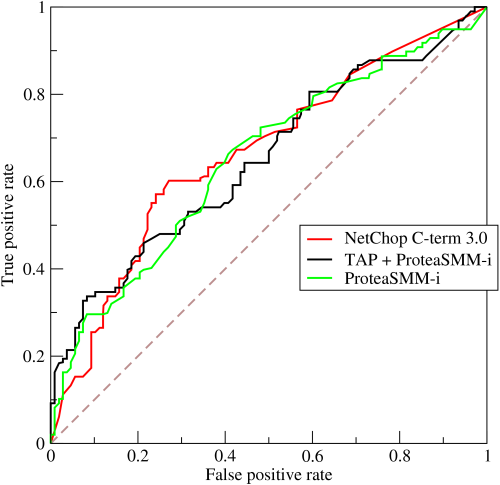
\includegraphics[keepaspectratio]{images/Roccurves.png}}
\end{column}
\end{columns}
\end{frame}

\begin{frame}{Precision-Recall Kurve}
\protect\phantomsection\label{precision-recall-kurve}
\begin{itemize}
\tightlist
\item
  \textbf{Alternative zur ROC-Kurve:}

  \begin{itemize}
  \tightlist
  \item
    Precision gegen Recall für verschiedene Schwellenwerte
  \end{itemize}
\item
  \textbf{Wann verwenden:}

  \begin{itemize}
  \tightlist
  \item
    Bei unausgewogenen Datensätzen
  \item
    Fokus auf positive Klasse
  \end{itemize}
\item
  \textbf{Interpretation:}

  \begin{itemize}
  \tightlist
  \item
    Besser: näher an oberer rechter Ecke
  \end{itemize}
\end{itemize}
\end{frame}

\begin{frame}{Overfitting vs.~Underfitting}
\protect\phantomsection\label{overfitting-vs.-underfitting}
\begin{itemize}
\tightlist
\item
  \textbf{Overfitting:}

  \begin{itemize}
  \tightlist
  \item
    Zu genaues Lernen (inkl. Rauschen)
  \item
    Gut im Training, schlecht im Test
  \end{itemize}
\item
  \textbf{Underfitting:}

  \begin{itemize}
  \tightlist
  \item
    Zu einfaches Modell
  \item
    Schlecht in Training und Test
  \end{itemize}
\item
  \textbf{Balance durch:}

  \begin{itemize}
  \tightlist
  \item
    Regularisierung
  \item
    Angemessene Modellkomplexität
  \end{itemize}
\end{itemize}
\end{frame}

\begin{frame}{Nächste Schritte}
\protect\phantomsection\label{nuxe4chste-schritte}
\begin{itemize}
\tightlist
\item
  Weitere Klassifikatoren testen (z.B. Entscheidungsbäume, SVM)
\item
  Optimierung der Textaufbereitung
\item
  Einsatz von Word Embeddings für fortgeschrittene Modelle
\end{itemize}
\end{frame}

\section{Sitzung 14: Abschluss}\label{sitzung-14-abschluss}

\begin{frame}{Lernziele dieser Sitzung}
\protect\phantomsection\label{lernziele-dieser-sitzung-12}
\begin{itemize}
\tightlist
\item
  Den gesamten Kurs strukturiert rekapitulieren
\item
  Den richtigen Test für eine gegebene Forschungsfrage auswählen
\item
  Ergebnisse korrekt berichten (APA-Style)
\end{itemize}
\end{frame}

\begin{frame}{Der rote Faden: Von der Frage zur Methode}
\protect\phantomsection\label{der-rote-faden-von-der-frage-zur-methode}
\pandocbounded{\includegraphics[keepaspectratio]{images/entscheidungsbaum.png}}
\end{frame}

\begin{frame}{Alle Tests auf einen Blick}
\protect\phantomsection\label{alle-tests-auf-einen-blick}
{\def\LTcaptype{none} % do not increment counter
\begin{longtable}[]{@{}
  >{\raggedright\arraybackslash}p{(\linewidth - 6\tabcolsep) * \real{0.2500}}
  >{\raggedright\arraybackslash}p{(\linewidth - 6\tabcolsep) * \real{0.2500}}
  >{\raggedright\arraybackslash}p{(\linewidth - 6\tabcolsep) * \real{0.2500}}
  >{\raggedright\arraybackslash}p{(\linewidth - 6\tabcolsep) * \real{0.2500}}@{}}
\toprule\noalign{}
\begin{minipage}[b]{\linewidth}\raggedright
Test
\end{minipage} & \begin{minipage}[b]{\linewidth}\raggedright
Abhängige Variable
\end{minipage} & \begin{minipage}[b]{\linewidth}\raggedright
Unabhängige Variable
\end{minipage} & \begin{minipage}[b]{\linewidth}\raggedright
Zweck
\end{minipage} \\
\midrule\noalign{}
\endhead
\textbf{t-Test} & Metrisch & Kategorial (2 Gruppen) &
Mittelwertsvergleich \\
\textbf{Chi-Quadrat} & Kategorial & Kategorial & Häufigkeiten /
Zusammenhang \\
\textbf{Korrelation} & Metrisch & Metrisch & Stärke des Zusammenhangs \\
\textbf{ANOVA} & Metrisch & Kategorial (\textgreater2 Gruppen) &
Mittelwertsvergleich \\
\textbf{Lin. Regression} & Metrisch & Metrisch / kategorial & Einfluss
\& Vorhersage \\
\textbf{Log. Regression} & Binär (0/1) & Metrisch / kategorial &
Wahrscheinlichkeit \\
\textbf{Mann-Whitney-U} & Ordinal / metrisch & Kategorial (2 Gruppen) &
Wie t-Test, nicht-parametrisch \\
\textbf{Kruskal-Wallis} & Ordinal / metrisch & Kategorial (\textgreater2
Gruppen) & Wie ANOVA, nicht-parametrisch \\
\bottomrule\noalign{}
\end{longtable}
}
\end{frame}

\begin{frame}{Ergebnisse korrekt berichten}
\protect\phantomsection\label{ergebnisse-korrekt-berichten}
\begin{itemize}
\tightlist
\item
  \textbf{Immer angeben}: Teststatistik, Freiheitsgrade, p-Wert,
  Effektgröße
\item
  \textbf{t-Test}: \emph{t}(28) = 2.45, \emph{p} = .02, \emph{d} = 0.89
\item
  \textbf{Chi-Quadrat}: χ²(2) = 8.24, \emph{p} = .016, Cramér's V = .23
\item
  \textbf{Korrelation}: \emph{r}(98) = .54, \emph{p} \textless{} .001
\item
  \textbf{ANOVA}: \emph{F}(2, 57) = 4.32, \emph{p} = .018, η² = .13
\end{itemize}
\end{frame}

\begin{frame}{Häufige Fehler in Bachelorarbeiten}
\protect\phantomsection\label{huxe4ufige-fehler-in-bachelorarbeiten}
\begin{itemize}
\tightlist
\item
  p-Wert ohne Effektgröße berichten
\item
  Korrelation als Kausalität interpretieren
\item
  Voraussetzungen nicht geprüft (Normalverteilung, Varianzhomogenität)
\item
  Signifikanz mit Relevanz gleichsetzen
\item
  Fehlende Werte ignorieren statt transparent machen
\item
  Daten nach dem Schauen anpassen (p-Hacking)
\end{itemize}
\end{frame}

\begin{frame}{Ein Wort zur Replikationskrise}
\protect\phantomsection\label{ein-wort-zur-replikationskrise}
\begin{itemize}
\tightlist
\item
  Viele publizierte Studien lassen sich nicht replizieren
\item
  Ursachen: p-Hacking, kleine Stichproben, Publication Bias
\item
  \textbf{Konsequenz für Ihre Arbeit}: Transparenz über Methoden,
  Voraussetzungsprüfung, Effektgrößen angeben
\item
  Vorregistrierung als Gold-Standard (für BA-Arbeiten optional, aber
  bekannt sein)
\end{itemize}
\end{frame}

\begin{frame}[fragile]{Stichprobengröße: Wie viele brauche ich?}
\protect\phantomsection\label{stichprobengruxf6uxdfe-wie-viele-brauche-ich}
\begin{itemize}
\tightlist
\item
  Zu kleine Stichproben → zu wenig Power → echte Effekte werden
  übersehen
\item
  Faustregel für Abschlussarbeiten: n ≥ 30 pro Gruppe (besser:
  Poweranalyse)
\item
  Power-Analyse in R:
\end{itemize}

\begin{Shaded}
\begin{Highlighting}[]
\FunctionTok{library}\NormalTok{(pwr)}
\CommentTok{\# Beispiel: t{-}Test, mittlerer Effekt (d=0.5), Power=0.80, α=0.05}
\FunctionTok{pwr.t.test}\NormalTok{(}\AttributeTok{d =} \FloatTok{0.5}\NormalTok{, }\AttributeTok{sig.level =} \FloatTok{0.05}\NormalTok{, }\AttributeTok{power =} \FloatTok{0.80}\NormalTok{, }\AttributeTok{type =} \StringTok{"two.sample"}\NormalTok{)}
\end{Highlighting}
\end{Shaded}
\end{frame}

\begin{frame}[fragile]{Fehlende Werte -- kein Tabuthema}
\protect\phantomsection\label{fehlende-werte-kein-tabuthema}
\begin{itemize}
\tightlist
\item
  Immer dokumentieren: Wie viele NAs? In welchen Variablen?
\item
  Strategien:

  \begin{itemize}
  \tightlist
  \item
    Komplette Beobachtungen (\texttt{na.omit()}) -- einfach, aber
    Datenverlust
  \item
    Mittelwert-/Medianimputation -- nur für MAR-Mechanismus
  \item
    Multiple Imputation (\texttt{mice}-Paket) -- Best Practice
  \end{itemize}
\item
  \textbf{Niemals}: NAs stillschweigend ignorieren
\end{itemize}
\end{frame}

\begin{frame}{Viel Erfolg!}
\protect\phantomsection\label{viel-erfolg}
\pandocbounded{\includegraphics[keepaspectratio]{images/marketoonist-big-data.png}}
\end{frame}

\section{Sitzung 9: Einfache Lineare
Regression}\label{sitzung-9-einfache-lineare-regression}

\begin{frame}{Von der Korrelation zur Regression}
\protect\phantomsection\label{von-der-korrelation-zur-regression}
\begin{itemize}
\tightlist
\item
  \textbf{Unterschied}: Korrelation beschreibt Zusammenhang, Regression
  ermöglicht Vorhersagen
\item
  \textbf{Abhängige vs.~unabhängige Variable}: Y als Funktion von X
\item
  \textbf{Lineare Beziehung}: Modellierung durch eine Gerade
\end{itemize}
\end{frame}

\begin{frame}{Das lineare Regressionsmodell}
\protect\phantomsection\label{das-lineare-regressionsmodell}
\begin{itemize}
\tightlist
\item
  \textbf{Grundgleichung}: \(Y = \beta_0 + \beta_1 X + \varepsilon\)
\item
  \textbf{Parameter}:

  \begin{itemize}
  \tightlist
  \item
    Achsenabschnitt (Intercept) \(\beta_0\): Wert von Y, wenn X = 0
  \item
    Steigung (Slope) \(\beta_1\): Änderung in Y bei Erhöhung von X um
    eine Einheit
  \item
    Fehlerterm \(\varepsilon\): Zufällige Abweichung (normalverteilt mit
    Mittelwert 0)
  \end{itemize}
\item
  \textbf{Kleinstquadrateschätzung}: Minimierung der quadrierten
  Residuen
\end{itemize}
\end{frame}

\begin{frame}{Durchführung in R}
\protect\phantomsection\label{durchfuxfchrung-in-r-1}
\begin{itemize}
\item
  \textbf{Einfache lineare Regression}:

  \section{Modell erstellen}\label{modell-erstellen}

  model \textless- lm(y \textasciitilde{} x, data = daten)

  \section{Zusammenfassung anzeigen}\label{zusammenfassung-anzeigen}

  summary(model)

  \section{Diagnostische Plots}\label{diagnostische-plots}

  par(mfrow = c(2, 2)) plot(model)
\end{itemize}
\end{frame}

\begin{frame}{Interpretation der Ergebnisse}
\protect\phantomsection\label{interpretation-der-ergebnisse}
\begin{itemize}
\tightlist
\item
  \textbf{Regressionskoeffizienten}: Bedeutung von Intercept und Slope
\item
  \textbf{Standardfehler der Koeffizienten}: Präzision der Schätzung
\item
  \textbf{t-Werte und p-Werte}: Signifikanz der Koeffizienten
\item
  \textbf{R²}: Erklärte Varianz bzw. Bestimmtheitsmaß

  \begin{itemize}
  \tightlist
  \item
    Interpretation: Anteil der Varianz in Y, der durch X erklärt wird
  \item
    Adjustiertes R²: Korrektur für die Anzahl der Prädiktoren
  \end{itemize}
\end{itemize}
\end{frame}

\begin{frame}{Voraussetzungen und Diagnostik}
\protect\phantomsection\label{voraussetzungen-und-diagnostik}
\begin{itemize}
\tightlist
\item
  \textbf{Linearität}: Beziehung sollte linear sein
\item
  \textbf{Normalverteilung der Residuen}: QQ-Plot zur Überprüfung
\item
  \textbf{Homoskedastizität}: Konstante Varianz der Residuen
\item
  \textbf{Unabhängigkeit der Beobachtungen}: Keine Autokorrelation
\item
  \textbf{Ausreißer und einflussreiche Beobachtungen}: Cook's Distance,
  Leverage
\end{itemize}
\end{frame}

\begin{frame}{Visualisierung von Regressionsmodellen}
\protect\phantomsection\label{visualisierung-von-regressionsmodellen}
\begin{itemize}
\item
  \textbf{Streudiagramm mit Regressionslinie}:

  library(ggplot2) ggplot(daten, aes(x = x, y = y)) + geom\_point() +
  geom\_smooth(method = ``lm'', se = TRUE) + theme\_minimal() +
  labs(title = ``Lineare Regression'', subtitle = paste(``R² ='',
  round(summary(model)\$r.squared, 3)))
\item
  \textbf{Residuenplots}:

  \section{Residuen gegen vorhergesagte
  Werte}\label{residuen-gegen-vorhergesagte-werte}

  ggplot(data.frame(fitted = fitted(model), residuals =
  residuals(model)), aes(x = fitted, y = residuals)) + geom\_point() +
  geom\_hline(yintercept = 0, linetype = ``dashed'', color = ``red'') +
  theme\_minimal() + labs(title = ``Residuen vs.~vorhergesagte Werte'')
\end{itemize}
\end{frame}

\begin{frame}{Praktische Anwendungsbeispiele}
\protect\phantomsection\label{praktische-anwendungsbeispiele-3}
\begin{itemize}
\tightlist
\item
  \textbf{Fairer Preis für gebrauchte Artikel}: Preisvorhersage
  basierend auf Alter, Zustand, etc.
\item
  \textbf{Verkaufsprognosen}: Vorhersage des Umsatzes basierend auf
  Werbeausgaben
\item
  \textbf{Biometrische Zusammenhänge}: z.B. Zusammenhang zwischen Größe
  und Gewicht
\end{itemize}
\end{frame}

\begin{frame}{Transformation nicht-linearer Beziehungen}
\protect\phantomsection\label{transformation-nicht-linearer-beziehungen}
\begin{itemize}
\item
  \textbf{Logarithmische Transformation}: Für exponentielle Beziehungen
\item
  \textbf{Quadratische Transformation}: Für U-förmige Beziehungen
\item
  \textbf{Box-Cox-Transformation}: Systematische Suche nach optimaler
  Transformation
\item
  \textbf{Beispiel in R}:

  ``` r \# Log-Transformation model\_log \textless- lm(log(y)
  \textasciitilde{} x, data = daten)

  \section{Quadratische
  Transformation}\label{quadratische-transformation}

  model\_quad \textless- lm(y \textasciitilde{} x + I(x\^{}2), data =
  daten)

  \section{Vergleich der Modelle mittels
  AIC}\label{vergleich-der-modelle-mittels-aic}

  AIC(model, model\_log, model\_quad)
\end{itemize}
\end{frame}

\section{Sitzung 10: Logistische
Regression}\label{sitzung-10-logistische-regression}

\begin{frame}{Was ist die logistische Regression?}
\protect\phantomsection\label{was-ist-die-logistische-regression}
\begin{itemize}
\tightlist
\item
  \textbf{Unterschied zur linearen Regression}: Binäre abhängige
  Variable
\item
  \textbf{Logit-Funktion}: Transformation von Wahrscheinlichkeiten in
  Log-Odds
\item
  \textbf{Grundgleichung}:
  \(\log\left(\frac{p}{1-p}\right) = \beta_0 + \beta_1 X\)
\item
  \textbf{Interpretation}: Odds Ratios statt direkter Effekte
\end{itemize}
\end{frame}

\begin{frame}[fragile]{Durchführung der logistischen Regression in R}
\protect\phantomsection\label{durchfuxfchrung-der-logistischen-regression-in-r}
\begin{itemize}
\tightlist
\item
  \textbf{Modellschätzung}:
\end{itemize}

\begin{Shaded}
\begin{Highlighting}[]
  \CommentTok{\# Logistische Regression}
\NormalTok{  logit\_model }\OtherTok{\textless{}{-}} \FunctionTok{glm}\NormalTok{(erfolg }\SpecialCharTok{\textasciitilde{}}\NormalTok{ x, }\AttributeTok{data =}\NormalTok{ daten, }\AttributeTok{family =}\NormalTok{ binomial)}
  \FunctionTok{summary}\NormalTok{(logit\_model)}

  \CommentTok{\# Odds Ratios berechnen}
  \FunctionTok{exp}\NormalTok{(}\FunctionTok{coef}\NormalTok{(logit\_model))}
\end{Highlighting}
\end{Shaded}

\begin{itemize}
\tightlist
\item
  \textbf{Vorhersagen und Evaluation}:
\end{itemize}

\begin{Shaded}
\begin{Highlighting}[]
  \CommentTok{\# Wahrscheinlichkeiten vorhersagen}
\NormalTok{  pred\_probs }\OtherTok{\textless{}{-}} \FunctionTok{predict}\NormalTok{(logit\_model, }\AttributeTok{type =} \StringTok{"response"}\NormalTok{)}

  \CommentTok{\# ROC{-}Kurve und AUC}
  \FunctionTok{library}\NormalTok{(pROC)}
\NormalTok{  roc\_curve }\OtherTok{\textless{}{-}} \FunctionTok{roc}\NormalTok{(daten}\SpecialCharTok{$}\NormalTok{erfolg, pred\_probs)}
  \FunctionTok{plot}\NormalTok{(roc\_curve)}
  \FunctionTok{auc}\NormalTok{(roc\_curve)}
\end{Highlighting}
\end{Shaded}
\end{frame}

\begin{frame}{Anwendungsbeispiele für logistische Regression}
\protect\phantomsection\label{anwendungsbeispiele-fuxfcr-logistische-regression}
\begin{itemize}
\tightlist
\item
  \textbf{Medizin}: Vorhersage von Krankheitsrisiken
\item
  \textbf{Marketing}: Conversion-Wahrscheinlichkeit von Kunden
\item
  \textbf{Kreditwesen}: Ausfallwahrscheinlichkeit bei Krediten
\end{itemize}
\end{frame}

\section{Sitzung 11: ANOVA und
Umfragedesign}\label{sitzung-11-anova-und-umfragedesign}

\begin{frame}{ANOVA-Grundlagen}
\protect\phantomsection\label{anova-grundlagen}
\begin{itemize}
\tightlist
\item
  \textbf{Vom t-Test zur ANOVA}: Natürliche Erweiterung für mehr als
  zwei Gruppen
\item
  \textbf{Varianzzerlegung}: Zwischen- vs.~Innerhalb-Gruppenvarianz
\item
  \textbf{F-Verteilung und F-Statistik}: Verhältnis der Varianzen
\item
  \textbf{Grundformel}:
  \(F = \frac{\text{Varianz zwischen Gruppen}}{\text{Varianz innerhalb Gruppen}}\)
\end{itemize}
\end{frame}

\begin{frame}[fragile]{Einfaktorielle ANOVA}
\protect\phantomsection\label{einfaktorielle-anova}
\begin{itemize}
\item
  \textbf{Voraussetzungen}:

  \begin{itemize}
  \tightlist
  \item
    Normalverteilung der Residuen
  \item
    Homoskedastizität (Varianzhomogenität)
  \item
    Unabhängigkeit der Beobachtungen
  \end{itemize}
\item
  \textbf{Durchführung in R}:

\begin{Shaded}
\begin{Highlighting}[]
\CommentTok{\# Einfaktorielle ANOVA}
\NormalTok{anova\_result }\OtherTok{\textless{}{-}} \FunctionTok{aov}\NormalTok{(werte }\SpecialCharTok{\textasciitilde{}}\NormalTok{ gruppe, }\AttributeTok{data =}\NormalTok{ daten)}
\FunctionTok{summary}\NormalTok{(anova\_result)}
\end{Highlighting}
\end{Shaded}
\end{itemize}
\end{frame}

\begin{frame}[fragile]{Post-hoc Tests}
\protect\phantomsection\label{post-hoc-tests-1}
\begin{itemize}
\item
  \textbf{Warum Post-hoc Tests?}: ANOVA sagt nur, dass Unterschiede
  existieren
\item
  \textbf{Tukey's HSD}: Häufig verwendeter Test für alle paarweisen
  Vergleiche
\item
  \textbf{Bonferroni-Korrektur}: Kontrolle des Alpha-Fehlers bei
  multiplen Vergleichen
\item
  \textbf{Durchführung in R}:

\begin{Shaded}
\begin{Highlighting}[]
\CommentTok{\# Tukey\textquotesingle{}s HSD}
\FunctionTok{TukeyHSD}\NormalTok{(anova\_result)}

\CommentTok{\# Alternativ mit dem Paket \textquotesingle{}multcomp\textquotesingle{}}
\FunctionTok{library}\NormalTok{(multcomp)}
\NormalTok{post\_hoc }\OtherTok{\textless{}{-}} \FunctionTok{glht}\NormalTok{(anova\_result, }\AttributeTok{linfct =} \FunctionTok{mcp}\NormalTok{(}\AttributeTok{gruppe =} \StringTok{"Tukey"}\NormalTok{))}
\FunctionTok{summary}\NormalTok{(post\_hoc)}
\end{Highlighting}
\end{Shaded}
\end{itemize}
\end{frame}

\begin{frame}[fragile]{Visualisierung von ANOVA-Ergebnissen}
\protect\phantomsection\label{visualisierung-von-anova-ergebnissen}
\begin{itemize}
\item
  \textbf{Boxplots mit Post-hoc-Informationen}:

\begin{Shaded}
\begin{Highlighting}[]
\FunctionTok{library}\NormalTok{(ggplot2)}
\FunctionTok{ggplot}\NormalTok{(daten, }\FunctionTok{aes}\NormalTok{(}\AttributeTok{x =}\NormalTok{ gruppe, }\AttributeTok{y =}\NormalTok{ werte, }\AttributeTok{fill =}\NormalTok{ gruppe)) }\SpecialCharTok{+}
  \FunctionTok{geom\_boxplot}\NormalTok{() }\SpecialCharTok{+}
  \FunctionTok{theme\_minimal}\NormalTok{() }\SpecialCharTok{+}
  \FunctionTok{labs}\NormalTok{(}\AttributeTok{title =} \StringTok{"Vergleich der Gruppen (ANOVA)"}\NormalTok{,}
       \AttributeTok{subtitle =} \StringTok{"F(2, 57) = 14.3, p \textless{} 0.001"}\NormalTok{)}
\end{Highlighting}
\end{Shaded}
\item
  \textbf{Interaktionsplots (für mehrfaktorielle ANOVA)}:

\begin{Shaded}
\begin{Highlighting}[]
\CommentTok{\# Für mehrfaktorielle ANOVA}
\FunctionTok{interaction.plot}\NormalTok{(daten}\SpecialCharTok{$}\NormalTok{faktor1, daten}\SpecialCharTok{$}\NormalTok{faktor2, daten}\SpecialCharTok{$}\NormalTok{werte,}
\NormalTok{                mean, }\AttributeTok{xlab =} \StringTok{"Faktor 1"}\NormalTok{, }\AttributeTok{ylab =} \StringTok{"Mittelwert"}\NormalTok{,}
                \AttributeTok{trace.label =} \StringTok{"Faktor 2"}\NormalTok{)}
\end{Highlighting}
\end{Shaded}
\end{itemize}
\end{frame}

\begin{frame}{Umfragen und Datenerhebung}
\protect\phantomsection\label{umfragen-und-datenerhebung}
\begin{block}{Grundsätzliche Aspekte der Datenerhebung}
\protect\phantomsection\label{grundsuxe4tzliche-aspekte-der-datenerhebung}
\begin{itemize}
\tightlist
\item
  \textbf{Primärdaten vs.~Sekundärdaten}: Vor- und Nachteile
\item
  \textbf{Quantitative vs.~qualitative Forschung}: Unterschiedliche
  Ansätze und Zielsetzungen
\item
  \textbf{Mixed Methods}: Kombination verschiedener Ansätze
\end{itemize}
\end{block}

\begin{block}{Umfragedesign}
\protect\phantomsection\label{umfragedesign}
\begin{itemize}
\tightlist
\item
  \textbf{Fragentypen}:

  \begin{itemize}
  \tightlist
  \item
    Offene vs.~geschlossene Fragen
  \item
    Single-Choice vs.~Multiple-Choice
  \item
    Likert-Skalen: Abstufungen und Best Practices
  \end{itemize}
\item
  \textbf{Skalendesign}:

  \begin{itemize}
  \tightlist
  \item
    Balance: Gleiche Anzahl positiver und negativer Optionen
  \item
    Neutraloption: Ja oder nein?
  \item
    Skalenlänge: 5-, 7- oder 10-Punkt-Skalen
  \end{itemize}
\end{itemize}
\end{block}

\begin{block}{Typische Fehlerquellen und Verzerrungen}
\protect\phantomsection\label{typische-fehlerquellen-und-verzerrungen}
\begin{itemize}
\tightlist
\item
  \textbf{Stichprobenverzerrung (Sampling Bias)}:

  \begin{itemize}
  \tightlist
  \item
    Convenience Sampling
  \item
    Self-Selection Bias
  \item
    Non-Response Bias
  \end{itemize}
\item
  \textbf{Antwortverzerrungen}:

  \begin{itemize}
  \tightlist
  \item
    Social Desirability Bias
  \item
    Acquiescence Bias (Ja-Sage-Tendenz)
  \item
    Extremity Bias (Tendenz zu Extremantworten)
  \item
    Central Tendency Bias (Tendenz zur Mitte)
  \end{itemize}
\end{itemize}
\end{block}

\begin{block}{Fallbeispiele von Verzerrungen}
\protect\phantomsection\label{fallbeispiele-von-verzerrungen}
\begin{itemize}
\tightlist
\item
  \textbf{Survivorship Bias}: Beobachtungen der ``Überlebenden''
\item
  \textbf{Verzerrung durch fehlende Daten}: Systematische vs.~zufällige
  fehlende Werte
\item
  \textbf{Kulturelle Unterschiede in der Beantwortung}: Internationale
  Studien
\end{itemize}
\end{block}

\begin{block}{Praktische Tipps für bessere Umfragen}
\protect\phantomsection\label{praktische-tipps-fuxfcr-bessere-umfragen}
\begin{itemize}
\tightlist
\item
  \textbf{Frageformulierung}: Klar, präzise, neutral
\item
  \textbf{Umfragelänge}: Ermüdung und Abbruchquoten
\item
  \textbf{Pretests durchführen}: Frühe Probleme erkennen
\item
  \textbf{Datenqualitätsprüfung}: Validierung während und nach der
  Erhebung
\end{itemize}
\end{block}

\begin{block}{Online-Tools und Software}
\protect\phantomsection\label{online-tools-und-software}
\begin{itemize}
\tightlist
\item
  \textbf{Umfragetools}: SurveyMonkey, Google Forms, LimeSurvey,
  Qualtrics
\item
  \textbf{Integration mit R}: Datenimport und -analyse
\end{itemize}
\end{block}
\end{frame}

\section{Sitzung 12: Abschluss und
Ausblick}\label{sitzung-12-abschluss-und-ausblick}

\begin{frame}{Zusammenfassung der wichtigsten Konzepte}
\protect\phantomsection\label{zusammenfassung-der-wichtigsten-konzepte}
\begin{itemize}
\tightlist
\item
  \textbf{Deskriptive Statistik}: Kennzahlen, Verteilungen,
  Visualisierung
\item
  \textbf{Inferenzstatistik}: Stichproben, Hypothesentests,
  Konfidenzintervalle
\item
  \textbf{Korrelation und Regression}: Zusammenhänge und Vorhersagen
\item
  \textbf{Kategoriale Datenanalyse}: Chi-Quadrat-Tests und
  Kontingenztabellen
\end{itemize}
\end{frame}

\begin{frame}{Integration der Methoden an praktischen Beispielen}
\protect\phantomsection\label{integration-der-methoden-an-praktischen-beispielen}
\begin{itemize}
\tightlist
\item
  \textbf{Fallstudie}: Durchführung einer vollständigen Datenanalyse

  \begin{enumerate}
  \tightlist
  \item
    Datenimport und -bereinigung
  \item
    Explorative Datenanalyse
  \item
    Hypothesenbildung
  \item
    Statistische Tests
  \item
    Modellierung (Regression)
  \item
    Interpretation und Berichterstattung
  \end{enumerate}
\end{itemize}
\end{frame}

\begin{frame}{Bewertungskriterien für die Hausarbeit}
\protect\phantomsection\label{bewertungskriterien-fuxfcr-die-hausarbeit}
\begin{itemize}
\tightlist
\item
  \textbf{Datenauswahl und -aufbereitung}: Sinnvolle Auswahl, korrekte
  Aufbereitung
\item
  \textbf{Methodik}: Angemessene Auswahl und korrekte Anwendung
  statistischer Verfahren
\item
  \textbf{Visualisierung}: Informative, korrekte und ästhetisch
  ansprechende Grafiken
\item
  \textbf{Interpretation}: Korrekte Deutung der Ergebnisse, Verständnis
  der Grenzen
\item
  \textbf{Dokumentation}: Klare, nachvollziehbare Darstellung der
  Analyse mit R Markdown
\end{itemize}
\end{frame}

\begin{frame}{Weiterführende statistische Methoden}
\protect\phantomsection\label{weiterfuxfchrende-statistische-methoden}
\begin{itemize}
\tightlist
\item
  \textbf{Mehrfaktorielle ANOVA}: Analyse mehrerer Einflussfaktoren und
  ihrer Interaktionen
\item
  \textbf{Multiple Regression}: Mehrere unabhängige Variablen
\item
  \textbf{Nicht-parametrische Verfahren}: Alternativen bei Verletzung
  der Normalverteilungsannahme
\item
  \textbf{Zeitreihenanalyse}: Analyse von Daten mit zeitlicher Struktur
\item
  \textbf{Faktorenanalyse}: Reduktion von Variablen auf latente Faktoren
\item
  \textbf{Clusteranalyse}: Identifikation von Gruppen in Daten
\item
  \textbf{Machine Learning}: Vorhersagemodelle und Klassifikation
\end{itemize}
\end{frame}

\begin{frame}{Praktische Hinweise für statistisches Arbeiten}
\protect\phantomsection\label{praktische-hinweise-fuxfcr-statistisches-arbeiten}
\begin{itemize}
\tightlist
\item
  \textbf{Reproduzierbarkeit}: Verwendung von R Markdown für
  nachvollziehbare Analysen
\item
  \textbf{Visualisierung vor Berechnung}: Daten immer zuerst
  visualisieren
\item
  \textbf{Datenvalidierung}: Überprüfung auf Ausreißer, fehlende Werte,
  unmögliche Werte
\item
  \textbf{Kritisches Denken}: Hinterfragen von Ergebnissen und Methoden
\item
  \textbf{Effektgrößen beachten}: Nicht nur auf p-Werte fixieren
\end{itemize}
\end{frame}

\begin{frame}{Ressourcen für das Selbststudium}
\protect\phantomsection\label{ressourcen-fuxfcr-das-selbststudium}
\begin{itemize}
\tightlist
\item
  \textbf{Bücher}:

  \begin{itemize}
  \tightlist
  \item
    ``R for Data Science'' von Hadley Wickham und Garrett Grolemund
  \item
    ``Discovering Statistics Using R'' von Andy Field
  \item
    ``An Introduction to Statistical Learning'' von James, Witten,
    Hastie und Tibshirani
  \end{itemize}
\item
  \textbf{Online-Ressourcen}:

  \begin{itemize}
  \tightlist
  \item
    RStudio Cheatsheets:
    \url{https://www.rstudio.com/resources/cheatsheets/}
  \item
    R-bloggers: \url{https://www.r-bloggers.com/}
  \item
    Datacamp-Kurse: \url{https://www.datacamp.com/courses/tech:r}
  \item
    Stackoverflow für R-spezifische Fragen
  \end{itemize}
\end{itemize}
\end{frame}

\begin{frame}{Datenkritisches Denken und ethische Aspekte}
\protect\phantomsection\label{datenkritisches-denken-und-ethische-aspekte}
\begin{itemize}
\tightlist
\item
  \textbf{Datenqualität und -herkunft}: Kritische Bewertung von
  Datenquellen
\item
  \textbf{Fallstricke der Statistik}: Häufige Fehlinterpretationen und
  wie man sie vermeidet
\item
  \textbf{Ethik in der Datenanalyse}: Datenschutz, Fairness, Transparenz
\item
  \textbf{Kommunikation statistischer Ergebnisse}: Verantwortungsvoller
  Umgang mit Daten in der Öffentlichkeit
\end{itemize}
\end{frame}

\begin{frame}{Abschlussdiskussion und Feedback}
\protect\phantomsection\label{abschlussdiskussion-und-feedback}
\begin{itemize}
\tightlist
\item
  \textbf{Offene Fragen}: Klärung verbleibender Unklarheiten
\item
  \textbf{Rückblick}: Was waren die wichtigsten Erkenntnisse?
\item
  \textbf{Ausblick}: Wie können die Studierenden die erlernten Methoden
  in ihren Abschlussarbeiten anwenden?
\item
  \textbf{Kursevaluation}: Feedback zum Seminar und
  Verbesserungsvorschläge
\end{itemize}
\end{frame}

\begin{frame}{Tipp des Tages: Statistische Fallstricke vermeiden}
\protect\phantomsection\label{tipp-des-tages-statistische-fallstricke-vermeiden}
\begin{itemize}
\tightlist
\item
  \textbf{Data Dredging (p-Hacking)}: Nicht so lange testen, bis ein
  signifikantes Ergebnis erscheint
\item
  \textbf{HARKing (Hypothesizing After Results are Known)}: Hypothesen
  vor der Analyse festlegen
\item
  \textbf{Cherry Picking}: Alle relevanten Ergebnisse berichten, nicht
  nur die ``schönen''
\item
  \textbf{Überinterpretation von p-Werten}: p \textless{} 0.05 bedeutet
  nicht ``wahr'' oder ``wichtig''
\item
  \textbf{Ignorieren von Effektgrößen}: Praktische Bedeutsamkeit ist oft
  wichtiger als statistische Signifikanz
\end{itemize}
\end{frame}




\end{document}
